\documentclass[12pt, a4paper, oneside]{report}
\usepackage{fontspec}
\usepackage{polyglossia}
\setdefaultlanguage{vietnamese}
\usepackage{indentfirst}
\setlength{\parindent}{1em}
\usepackage{geometry} 
\geometry{
  a4paper,
  top=2.5cm,
  bottom=3cm,
  left=3.5cm,
  right=2cm
}
\usepackage{setspace} 
\setstretch{1.5}
\usepackage{fancyhdr}
\usepackage{fancybox}

\usepackage{amsmath, amssymb, amsthm} 
\usepackage{mathtools}
\usepackage{bm} 
\usepackage{mathrsfs} 
\usepackage{siunitx}

\usepackage{graphicx}
\usepackage{caption}
\usepackage{subcaption}
\usepackage{float}
\usepackage{booktabs} 
\usepackage{array}
\usepackage{tikz}
\usetikzlibrary{calc}
\usepackage{multirow}

\newtheoremstyle{mycustomstyle}
  {\topsep} 
  {\topsep}  
  {\normalfont}  
  {}                 
  {\bfseries}            
  {.}      
  {.5em}    
  {#1 #2\thmnote{ \mdseries\textit{(#3)}}} 

\theoremstyle{mycustomstyle}
\newtheorem{definition}{Định nghĩa}[section]
\newtheorem{remark}[definition]{Nhận xét}
\newtheorem{proposition}[definition]{Mệnh đề}
\newtheorem{convention}[definition]{Quy ước}
\newtheorem{example}[definition]{Ví dụ}
\newtheorem{corollary}[definition]{Hệ quả}
\newtheorem{theorem}[definition]{Định lý}
\newtheorem{postulate}[definition]{Tiên đề}

\usepackage{enumitem}
\usepackage{algorithm}
\usepackage[noend]{algpseudocode}
\usepackage[most]{tcolorbox}
\usepackage{mdframed}
\usepackage{framed}

\usepackage{xcolor}
\definecolor{mykeywordcolor}{RGB}{15,129,3}  
\definecolor{mycommentcolor}{RGB}{199,114,139}
\definecolor{mybackgroundcolor}{RGB}{245,245,245}

\usepackage{listings}
\lstset{
    language=Python,
    basicstyle=\ttfamily\footnotesize,
    keywordstyle=\color{blue},
    stringstyle=\color{red},
    commentstyle=\color{mycommentcolor},
    backgroundcolor=\color{mybackgroundcolor},
    frame=single,
    breaklines=true,
    tabsize=4,
    showstringspaces=false,
    literate={á}{{\'a}}1 {à}{{\`a}}1 {ả}{{\h{a}}}1 {ã}{{\~a}}1 {ạ}{{\d{a}}}1,
    escapeinside=||,
    extendedchars=true
}

\usepackage{minted}
\setminted{
    linenos=true,
    breaklines=true,
    frame=single,
    framesep=2mm,
    fontsize=\small,
    tabsize=4,
    numbersep=5pt,
}

\usepackage{hyperref} 
\hypersetup{
    colorlinks=true,
    linkcolor=black,
    urlcolor=cyan,
    citecolor=blue
}

\begin{document}

% Gọi file bìa
% --- TRANG BÌA CHÍNH ---
\begin{titlepage}
    \begin{tikzpicture}[overlay, remember picture]
        \draw [line width=2pt] 
            ($ (current page.north west) + (3.5cm,-2.5cm) $) 
            rectangle 
            ($ (current page.south east) + (-2.0cm,3.0cm) $);
        \draw [line width=0.5pt] 
            ($ (current page.north west) + (3.5cm + 1mm, -2.5cm - 1mm) $) 
            rectangle 
            ($ (current page.south east) + (-2.0cm - 1mm, 3.0cm + 1mm) $);
    \end{tikzpicture}

    \centering
    {\fontsize{13}{15}\selectfont
      ĐẠI HỌC QUỐC GIA HÀ NỘI\\[2pt]
      TRƯỜNG ĐẠI HỌC KHOA HỌC TỰ NHIÊN\\[2pt]
    }
    {\fontsize{13}{15}\selectfont\bfseries
      KHOA TOÁN - CƠ - TIN HỌC
    }

    \vspace{2.5cm}
    {\fontsize{14}{17}\selectfont\bfseries
      Nguyễn Tiến Đạt
    }

    \vspace{3cm}
    {\fontsize{18}{22}\selectfont\bfseries
      Cơ sở toán học của xác suất lượng tử\\[4pt]
      và ứng dụng trong mô phỏng số thuật toán Deutsch-Jozsa
    }

    \vspace{2.5cm}
    {\fontsize{14}{17}\selectfont
      Khóa luận tốt nghiệp đại học hệ chính quy\\[4pt]
      Ngành Toán Tin\\[4pt]
      (Chương trình đào tạo chuẩn)
    }

    \vfill
    {\fontsize{14}{17}\selectfont\bfseries
      Hà Nội - 2026
    }
    \vspace{0.7cm}
\end{titlepage}

% --- TRANG BÌA PHỤ ---
\begin{titlepage}
    \begin{tikzpicture}[overlay, remember picture]
        \draw [line width=2pt] 
            ($ (current page.north west) + (3.5cm,-2.5cm) $) 
            rectangle 
            ($ (current page.south east) + (-2.0cm,3.0cm) $);
        \draw [line width=0.5pt] 
            ($ (current page.north west) + (3.5cm + 1mm, -2.5cm - 1mm) $) 
            rectangle 
            ($ (current page.south east) + (-2.0cm - 1mm, 3.0cm + 1mm) $);
    \end{tikzpicture}

    \centering
    {\fontsize{13}{15}\selectfont
      ĐẠI HỌC QUỐC GIA HÀ NỘI\\[2pt]
      TRƯỜNG ĐẠI HỌC KHOA HỌC TỰ NHIÊN\\[2pt]
    }
    {\fontsize{13}{15}\selectfont\bfseries
      KHOA TOÁN - CƠ - TIN HỌC
    }

    \vspace{2.5cm}
    {\fontsize{14}{17}\selectfont\bfseries
      Nguyễn Tiến Đạt
    }

    \vspace{3cm}
    {\fontsize{18}{22}\selectfont\bfseries
      Cơ sở toán học của xác suất lượng tử\\[4pt]
      và ứng dụng trong mô phỏng số thuật toán Deutsch-Jozsa
    }

    \vspace{2.5cm}
    {\fontsize{14}{17}\selectfont
      Khóa luận tốt nghiệp đại học hệ chính quy\\[4pt]
      Ngành Toán Tin\\[4pt]
      (Chương trình đào tạo chuẩn)
    }

    \vspace{1.2cm}
    {\fontsize{14}{17}\selectfont\bfseries
      Cán bộ hướng dẫn: PGS.TS. Nguyễn Tiến Dũng
    }

    \vfill
    {\fontsize{14}{17}\selectfont\bfseries
      Hà Nội - 2026
    }
    \vspace{0.7cm}
\end{titlepage}

\pagestyle{fancy} % Tạo header
\fancyhead[L]{\itshape \nouppercase{\rightmark}}
\fancyhead[R]{}

\newpage % Tạo một trang rỗng
\mbox{}
\newpage

\chapter*{}
\begin{center}
    {\fontsize{20}{24}\selectfont\bfseries LỜI CẢM ƠN}
\end{center}
\addcontentsline{toc}{chapter}{Lời cảm ơn}
\vspace{1cm}
Lời đầu tiên của khóa luận, em xin gửi lời cảm ơn tới các thầy cô giáo của khoa Toán - Cơ - Tin học, trường Đại học Khoa học Tự nhiên, Đại học Quốc gia Hà Nội đã tạo điều kiện thuận lợi để em được học tập, rèn luyện và tích lũy kiến thức, kỹ năng trong suốt quá trình học tập, qua đó giúp em hoàn thành khóa luận này.

Đặc biệt, em xin bày tỏ lòng biết ơn sâu sắc tới giảng viên hướng dẫn của mình, PGS.TS. Nguyễn Tiến Dũng. Thầy đã tận tâm hướng dẫn, hỗ trợ và cung cấp cho em những kiến thức, tài liệu tham khảo cùng định hướng nghiên cứu cần thiết xuyên suốt quá trình thực hiện và hoàn thành khóa luận này.

Cuối cùng, em xin gửi lời cảm ơn chân thành tới gia đình và bạn bè, những người đã luôn tin tưởng, động viên và khích lệ em trong suốt những năm học đại học cũng như trong quá trình hoàn thiện khóa luận tốt nghiệp.

Do thời gian và kiến thức còn hạn chế, khóa luận không thể tránh khỏi những thiếu sót. Em kính mong nhận được sự chỉ bảo và góp ý của quý thầy cô để khóa luận được hoàn thiện hơn.

\textit{Em xin chân thành cảm ơn!}

\begin{flushright}
    \textit{Hà Nội, tháng 05 năm 2026} \\
    Sinh viên\\
    Nguyễn Tiến Đạt
\end{flushright}

\tableofcontents % Mục lục

\renewcommand{\listfigurename}{Danh sách hình vẽ}
\listoffigures

\newpage
\renewcommand{\listtablename}{Danh sách bảng}
\listoftables

\newpage
\chapter*{}
\begin{center}
    {\fontsize{20}{24}\selectfont\bfseries Danh sách các thuật ngữ viết tắt}
\end{center}
\begin{table}[h]
\centering
\renewcommand{\arraystretch}{1.3}
\begin{tabular}{|c|l|l|p{5.5cm}|}
\hline
\textbf{STT} & \textbf{Từ viết tắt} & \textbf{Từ đầy đủ} & \textbf{Ý nghĩa} \\
\hline
1 & CCNOT & Controlled-Controlled-NOT & Cổng Toffoli ba qubit \\
\hline
2 & CNOT  & Controlled-NOT            & Cổng NOT có điều khiển \\
\hline
3 & QC    & Quantum Computing         & Tính toán lượng tử \\
\hline
4 & QFT   & Quantum Fourier Transform & Biến đổi Fourier lượng tử \\
\hline
5 & qubit & quantum bit               & Bit lượng tử \\
\hline
\end{tabular}
\end{table}

\chapter*{}
\begin{center}
    {\fontsize{20}{24}\selectfont\bfseries MỞ ĐẦU}
\end{center}
\addcontentsline{toc}{chapter}{Mở đầu}
\markboth{}{}
\vspace{1cm} 
Năm 1985, David Deutsch đã đặt ra một câu hỏi tưởng chừng triết học: liệu có tồn tại một máy tính vật lý có thể mô phỏng hiệu quả mọi quá trình vật lý trong tự nhiên không? Câu trả lời mà ông đưa ra rằng, máy tính đó phải hoạt động theo các nguyên lý của cơ học lượng tử. Từ đó đã đặt nền móng cho một lĩnh vực hoàn toàn mới: tính toán lượng tử (quantum computation). Bảy năm sau, Deutsch và Jozsa đã phát triển một thuật toán để chứng minh một máy tính lượng tử có thể giải một bài toán cụ thể chỉ trong một bước duy nhất, trong khi bất kỳ thuật toán cổ điển tất định nào cũng cần đến hàng triệu bước khi kích thước đầu vào tăng lên.

Bốn thập kỷ sau, tính toán lượng tử đang chuyển dịch mạnh mẽ từ lý thuyết sang hiện thực. IBM, Google và IonQ lần lượt công bố các hệ thống vượt mốc 1000 qubit trong giai đoạn 2023–2025, đánh dấu bước chuyển từ thí nghiệm phòng lab sang nền tảng có thể tiếp cận qua đám mây. Tại Việt Nam, sự quan tâm đến lĩnh vực này đang gia tăng cùng với các chương trình đầu tư vào nhân lực nghiên cứu lượng tử, nhưng tài liệu tiếng Việt kết nối chặt chẽ giữa nền tảng toán học và lập trình lượng tử thực tiễn vẫn còn rất hạn chế.

Để hiểu tại sao tính toán lượng tử có thể vượt trội so với tính toán cổ điển, cần phải hiểu nền tảng toán học đằng sau nó. Máy tính cổ điển xử lý thông tin dưới dạng bit nhận giá trị 0 hoặc 1 -- giống như công tắc chỉ có thể tắt hoặc bật. Máy tính lượng tử thay thế bit bằng qubit (quantum bit), có thể tồn tại đồng thời ở cả hai trạng thái cho đến khi được đo, gọi là chồng chất lượng tử (quantum superposition). Xác suất của kết quả đo không phải là một con số tùy ý mà được xác định bởi biên độ xác suất (probability amplitude) trong không gian Hilbert phức, các biên độ này có thể triệt tiêu nhau như sóng, tạo ra hiện tượng giao thoa lượng tử (quantum interference) mà xác suất cổ điển không thể giải thích được. Chính yếu tố đó là cơ sở cho thuật toán Deutsch-Jozsa. Nền tảng toán học đầy đủ của lý thuyết này bao gồm: không gian Hilbert, toán tử tuyến tính, hệ tiên đề và quy tắc Born đều được trình bày có tính hệ thống trong các tài liệu về xác suất lượng tử và tính toán lượng tử. Tuy nhiên, các hướng dẫn lập trình lượng tử thực tiễn lại hiếm khi giải thích cơ sở đó. Điều đó tạo ra một rào cản lớn, khiến người học chỉ có thể thao tác lập trình mà thiếu đi sự hiểu biết sâu sắc về nguyên lý vận hành cốt lõi của các mạch lượng tử.

Mục tiêu của khóa luận này là xây dựng một trình bày toán học về cơ sở xác suất lượng tử từ không gian Hilbert và tiên đề cơ học lượng tử đến lý thuyết phép đo,  từ đó phân tích thuật toán Deutsch-Jozsa và kiểm chứng qua mô phỏng số với Python và Qiskit. Thuật toán Deutsch-Jozsa được chọn vì nó là đối tượng lý tưởng để minh họa trọn vẹn các khái niệm cốt lõi bao gồm: chồng chất, giao thoa, oracle lượng tử (quantum oracle) và phép đo lượng tử. Đây là mô hình phù hợp để phân tích chi tiết và trình bày một cách hệ thống trong khuôn khổ của một khóa luận tốt nghiệp đại học.

Khóa luận được tổ chức thành ba chương chính.
\begin{itemize}
    \item Chương 1 xây dựng nền tảng toán học của cơ học lượng tử, bao gồm không gian Hilbert, các lớp toán tử tuyến tính quan trọng, hệ tiên đề lượng tử.
    \item Chương 2 xây dựng mô hình tính toán lượng tử: qubit, các cổng lượng tử phổ biến và cấu trúc mạch.
    \item Chương 3 phân tích thuật toán Deutsch-Jozsa và kiểm chứng qua mô phỏng số.
\end{itemize}  

Trong quá trình thực hiện khóa luận, có một số nội dung được sử dụng các công cụ trí tuệ nhân tạo như một trợ lý soạn thảo và tra cứu: hỗ trợ diễn đạt lại các nội dung được dịch ra từ tài liệu tham khảo, gợi ý cấu trúc trình bày và kiểm tra tính nhất quán của ký hiệu toán học. Bản thân em cam kết toàn bộ nội dung toán học, diễn giải lập luận và kết quả mô phỏng đều được tự xây dựng, tổng hợp và chịu trách nhiệm.

\pagestyle{fancy} 
\fancyhead[L]{\itshape \nouppercase{\rightmark}}

\chapter{Cơ sở toán học của xác suất lượng tử}
Chương này xây dựng nền tảng toán học cho phần còn lại của khóa luận theo ba phần kế tiếp: mục~\ref{sec:hilbert} giới thiệu không gian Hilbert và ký hiệu Dirac như ngôn ngữ toán học nền tảng; mục~\ref{sec:operators} trình bày về lý thuyết toán tử tuyến tính như Hermitian, unitary, định lý phổ và tích tensor, đây đều là các công cụ sẽ được dùng trực tiếp trong hệ tiên đề và mạch lượng tử; mục~\ref{sec:postulates} gắn ý nghĩa vật lý cho các công cụ đại số đó qua bốn tiên đề Dirac--von Neumann. Để xây dựng nên cấu trúc toán học chặt chẽ này, nội dung của chương được tham khảo chính từ giáo trình cơ sở của Nielsen \& Chuang~\cite{ref5} và tài liệu giảng dạy về tính toán lượng tử của Maassen~\cite{ref4}.

\section{Không gian Hilbert và ký hiệu Dirac}
\label{sec:hilbert}
Để xây dựng một khung toán học vững chắc cho cơ học lượng tử và lý thuyết thông tin lượng tử, các trạng thái vật lý và quá trình đo lường được mô hình hóa dựa trên lý thuyết không gian Hilbert, kết hợp với hệ thống ký hiệu bra-ket do Paul Dirac đề xuất. Hai công cụ này cùng nhau tạo thành ngôn ngữ toán học chuẩn hóa của vật lý lượng tử hiện đại.

\begin{definition}[Không gian Hilbert] 
Không gian Hilbert $\mathcal{H}$ được định nghĩa là một không gian vectơ trên trường số phức $\mathbb{C}$, được trang bị một phép tích trong (inner product) Hermite xác định dương. Phép tích trong là một ánh xạ từ $\mathcal{H} \times \mathcal{H}$ sang $\mathbb{C}$, biến đổi hai vectơ thành một đại lượng vô hướng phức. Đối với các vectơ tùy ý $|\psi\rangle, |\chi\rangle, |\phi\rangle \in \mathcal{H}$ và các đại lượng vô hướng $\alpha, \beta \in \mathbb{C}$, phép tích trong phải thỏa mãn ba tiên đề sau:
\begin{itemize}
    \item Tính tuyến tính đối với đối số thứ hai: $\langle \psi | (\alpha \chi + \beta \phi) \rangle = \alpha \langle \psi | \chi \rangle + \beta \langle \psi | \phi \rangle$.
    \item Tính đối xứng liên hợp Hermite: $\langle \psi | \chi \rangle = \overline{\langle \chi | \psi \rangle}$, trong đó dấu gạch ngang biểu diễn phép lấy liên hợp phức.
    \item Tính xác định dương: $\langle \psi | \psi \rangle \ge 0$, và đẳng thức xảy ra khi và chỉ khi $\psi$ là vectơ không.
\end{itemize}
\end{definition}

\begin{remark} [Chuẩn và Tính đầy đủ] Từ định nghĩa tích trong, ta rút ra hai tính chất nền tảng của không gian Hilbert:
\begin{enumerate}
    \item Chuẩn (Norm): Từ tích trong, chuẩn của một vectơ $|\psi\rangle$ được định nghĩa bằng $\|\psi\| = \sqrt{\langle \psi | \psi \rangle}$, đặc trưng cho ``độ dài" hình học của vectơ đó trong không gian.
    
    \item Tính đầy đủ (Completeness): Đối với các hệ vô hạn chiều, không gian tích trong phải thỏa mãn thêm điều kiện mọi dãy Cauchy trong $\mathcal{H}$ đều hội tụ về một phần tử thuộc chính $\mathcal{H}$. Nếu điều kiện này không được đáp ứng, cấu trúc toán học chỉ được gọi là không gian tiền-Hilbert (pre-Hilbert space). Trong bối cảnh tính toán và thông tin lượng tử hữu hạn chiều, không gian Hilbert đồng nhất với không gian vectơ phức $\mathbb{C}^n$, nơi phép tích trong thông thường luôn đảm bảo tính đầy đủ.
\end{enumerate}
\end{remark}

\begin{convention}[Ký hiệu Dirac] 
Hệ thống ký hiệu Dirac phân tách cấu trúc vectơ thành hai thành phần đối ngẫu nhằm biểu diễn các trạng thái vật lý. Cụ thể, hai thành phần này bao gồm:
\begin{itemize}
    \item Ký hiệu ket $|\psi\rangle$: đại diện cho một vectơ trạng thái trong $\mathcal{H}$; dưới dạng ma trận, đây là một vectơ cột chứa các biên độ xác suất phức.
    \item Ký hiệu bra $\langle\psi|$: đại diện cho vectơ đối ngẫu trong không gian đối ngẫu $\mathcal{H}^*$, hoạt động như một toán tử tuyến tính ánh xạ từ $\mathcal{H}$ sang $\mathbb{C}$ thông qua $\langle \psi | (|\chi\rangle) \equiv \langle \psi | \chi \rangle$; dưới dạng ma trận, bra là vectơ hàng thu được bằng phép chuyển vị liên hợp của ket tương ứng.
\end{itemize}
Sự kết hợp $\langle \psi | \chi \rangle$ chính là tích trong giữa hai vectơ trạng thái.
\end{convention}

\begin{definition}[Hệ trực chuẩn và cơ sở] 
Để biểu diễn các trạng thái cụ thể trong $\mathcal{H}$, cần thiết lập một cơ sở trực chuẩn. Một tập hợp các vectơ $\{|i\rangle\}$ được gọi là hệ trực chuẩn nếu thỏa mãn điều kiện $\langle i|j\rangle = \delta_{ij}$, với $\delta_{ij}$ là hàm Kronecker. 
$$\langle i|j\rangle = \delta_{ij}=\begin{cases} 
1 & \text{nếu } i = j \\ 
0 & \text{nếu } i \neq j 
\end{cases}$$
\end{definition}

\begin{remark} Đối với mọi không gian vectơ hữu hạn chiều, cơ sở trực chuẩn $\{|a\rangle\}$ (thỏa mãn $\langle i|j\rangle = \delta_{ij}$) luôn tồn tại và có thể được xây dựng từ một tập vectơ độc lập tuyến tính thông qua quá trình trực giao hóa Gram–Schmidt.
\end{remark}

\begin{proposition}
Khi cơ sở đã được xác định, một trạng thái lượng tử tổng quát $|\psi\rangle$ được phân tích dưới dạng tổ hợp tuyến tính: 
$$|\psi\rangle = \sum_{a \in A} \alpha_a |a\rangle$$ 
Trong đó, $\alpha_a \in \mathbb{C}$ là các biên độ xác suất phức và $|\alpha_a|^2$ là xác suất để hệ được đo thấy ở trạng thái cơ sở $|a\rangle$ (theo diễn giải Born). Điều kiện chuẩn hóa $\|\psi\| = 1$ đảm bảo tổng các xác suất này bằng 1.
\end{proposition}

\begin{framed}
\textbf{Ví dụ minh họa:} Ta xét một hệ có 3 trạng thái cơ sở trực chuẩn $|e_1\rangle, |e_2\rangle, |e_3\rangle$. Một trạng thái $|\psi\rangle$ có thể được biểu diễn như sau:
$$|\psi\rangle = \frac{1}{\sqrt{2}}|e_1\rangle + \frac{1}{2}|e_2\rangle + \frac{1}{2}|e_3\rangle$$
\begin{itemize}
    \item Xác suất: Khi đo đạc, hệ có $50\%$ xác suất rơi vào trạng thái $|e_1\rangle$ ($|\frac{1}{\sqrt{2}}|^2 = 0.5$) và mỗi trạng thái $|e_2\rangle, |e_3\rangle$ chiếm $25\%$ xác suất ($|\frac{1}{2}|^2 = 0.25$).
    \item Chuẩn hóa: Tổng các xác suất là $0.5 + 0.25 + 0.25 = 1$, thỏa mãn tính bảo toàn xác suất của hệ lượng tử.
\end{itemize}
\end{framed}

Bên cạnh việc biểu diễn các trạng thái, hệ thống ký hiệu Dirac cung cấp một phương thức tự nhiên để định nghĩa các toán tử tuyến tính thông qua khái niệm tích ngoài (outer product). 
\begin{definition}[Tích ngoài] Một tích ngoài, ký hiệu là $|w\rangle\langle v|$, thiết lập một toán tử ánh xạ giữa các không gian Hilbert, thực hiện biến đổi một vectơ $|v'\rangle$ theo quy tắc:
$$(|w\rangle\langle v|)|v'\rangle = |w\rangle\langle v|v'\rangle$$
Trong đó, tích nội $\langle v|v'\rangle$ đóng vai trò là một hệ số phức (biên độ) điều chỉnh độ lớn của vectơ kết quả $|w\rangle$.
\end{definition}

\begin{proposition}[Hệ thức đầy đủ] Với bất kỳ cơ sở trực chuẩn $\{|i\rangle\}$ nào, tổng các tích ngoài của tất cả các vectơ cơ sở tương đương với toán tử đồng nhất $I$:$$\sum_i |i\rangle\langle i| = I$$Hệ thức này cho phép phân tích một trạng thái lượng tử bất kỳ thành tổng các hình chiếu của nó trên tập cơ sở.
\end{proposition}

\begin{framed}
\textbf{Ví dụ minh họa:} Ta xét không gian Hilbert hai chiều với cơ sở trực chuẩn $\{|0\rangle, |1\rangle\}$ (các trạng thái cơ sở này sẽ được thảo luận chi tiết trong chương sau dưới khái niệm qubit). Trong đó:$$|0\rangle = \begin{pmatrix} 1 \\ 0 \end{pmatrix}, \quad |1\rangle = \begin{pmatrix} 0 \\ 1 \end{pmatrix}$$
\textit{Định nghĩa toán tử bằng tích ngoài:} xét toán tử hình chiếu lên trạng thái $|0\rangle$, ký hiệu là $\hat{P}_0 = |0\rangle\langle 0|$. Khi tác động lên một trạng thái bất kỳ $|\psi\rangle = \alpha|0\rangle + \beta|1\rangle$:
$$\hat{P}_0 |\psi\rangle = (|0\rangle\langle 0|) (\alpha|0\rangle + \beta|1\rangle) = \alpha|0\rangle\langle 0|0\rangle + \beta|0\rangle\langle 0|1\rangle$$Vì $\langle 0|0\rangle = 1$ và $\langle 0|1\rangle = 0$, kết quả là $\alpha|0\rangle$. Toán tử đã \textit{lọc} và chỉ giữ lại thành phần của trạng thái $|0\rangle$.\\
\textit{Chứng minh hệ thức đầy đủ:} các toán tử hình chiếu tương ứng được biểu diễn dưới dạng ma trận:
$$|0\rangle\langle 0| = \begin{pmatrix} 1 \\ 0 \end{pmatrix} \begin{pmatrix} 1 & 0 \end{pmatrix} = \begin{pmatrix} 1 & 0 \\ 0 & 0 \end{pmatrix}; \quad |1\rangle\langle 1| = \begin{pmatrix} 0 \\ 1 \end{pmatrix} \begin{pmatrix} 0 & 1 \end{pmatrix} = \begin{pmatrix} 0 & 0 \\ 0 & 1 \end{pmatrix}$$
Khi đó, hệ thức đầy đủ được thỏa mãn:$$|0\rangle\langle 0| + |1\rangle\langle 1| = \begin{pmatrix} 1 & 0 \\ 0 & 1 \end{pmatrix} = I$$
\end{framed}

Trong cơ học lượng tử, tích ngoài đóng vai trò nền tảng để xây dựng các \textbf{toán tử chiếu trực giao} (orthogonal projection operators) -- một thành phần trung tâm trong tiên đề đo lường.
\begin{definition}[Toán tử chiếu trực giao] Xét không gian con $k$ chiều được sinh bởi tập vectơ cơ sở trực chuẩn $\{|1\rangle, \dots, |k\rangle\}$, toán tử chiếu $P$ lên không gian này được định nghĩa bởi:
\[
P = \sum_{i=1}^k |i\rangle\langle i|
\]
\end{definition}

\begin{proposition} Toán tử chiếu trực giao được đặc trưng bởi hai tính chất đại số:
\begin{itemize}
    \item \textbf{Tính Hermite ($P^\dagger = P$):} Đảm bảo phép chiếu là trực giao và các giá trị kỳ vọng (xác suất) luôn là số thực, đáp ứng yêu cầu của một đại lượng quan sát vật lý.
    \item \textbf{Tính lũy đẳng ($P^2 = P$):} Phản ánh bản chất của phép chiếu; một trạng thái khi đã được chiếu vào không gian con sẽ không thay đổi dưới các tác động trùng lặp của cùng một toán tử.
\end{itemize}
Theo tiên đề đo lường, xác suất $\text{Pr}[X = s]$ thu được kết quả $s$ khi đo hệ đang ở trạng thái $|\psi\rangle$ được xác định bởi:
\[
\text{Pr}[X = s] = \langle\psi| P_s |\psi\rangle
\]
trong đó $P_s$ là toán tử chiếu tương ứng với kết quả $s$.
\end{proposition}

\begin{framed} \textbf{Ví dụ minh họa:} Xét qubit $|\psi\rangle = \frac{\sqrt{3}}{2}|0\rangle + \frac{1}{2}|1\rangle$. Xác suất thu được kết quả $0$ khi đo theo toán tử chiếu $P_0 = |0\rangle\langle 0|$ là:$$ \text{Pr}[0] = \langle\psi| P_0 |\psi\rangle = |\langle 0|\psi\rangle|^2 = \left(\frac{\sqrt{3}}{2}\right)^2 = \frac{3}{4} $$Về mặt hình học, xác suất này chính là bình phương độ dài hình chiếu của $|\psi\rangle$ lên phương của $|0\rangle$.
\end{framed}

\section{Toán tử tuyến tính: Hermitian, Unitary và định lý phổ}
\label{sec:operators}
Trong cơ học lượng tử, nếu các vectơ trạng thái mô tả trạng thái của một hệ vật lý, thì các toán tử tuyến tính đóng vai trò biểu diễn các đại lượng vật lý có thể quan sát được cũng như sự tiến hóa của hệ theo thời gian.
\begin{definition}[Toán tử tuyến tính]
Một toán tử tuyến tính $A$ trên không gian Hilbert $\mathcal{H}$ là một ánh xạ $A: \mathcal{H} \to \mathcal{H}$ thỏa mãn:
$$ A(\alpha |\psi\rangle + \beta |\phi\rangle) = \alpha A|\psi\rangle + \beta A|\phi\rangle $$
với mọi $|\psi\rangle, |\phi\rangle \in \mathcal{H}$ và $\alpha, \beta \in \mathbb{C}$.
\end{definition}

\begin{definition}[Toán tử liên hợp]
Gắn liền với $A$ là toán tử liên hợp $A^\dagger$, xác định duy nhất qua hệ thức $\langle v | A | w \rangle = \langle A^\dagger v | w \rangle, \forall |v\rangle, |w\rangle \in \mathcal{H}$. Dựa trên khái niệm này, các lớp toán tử chủ chốt trong cơ học lượng tử được phân loại theo mối liên hệ giữa $A$ và $A^\dagger$, cụ thể là các toán tử tự liên hợp (biểu diễn đại lượng quan sát) và toán tử unitary (biểu diễn sự tiến hóa trạng thái).
\end{definition}

\begin{definition}[Toán tử Hermitian]
Một toán tử tuyến tính $A$ trên không gian Hilbert $\mathcal{H}$ được gọi là
\textbf{Hermitian} (hay \textbf{tự liên hợp}) nếu
$$A^\dagger = A,$$
tức là $\langle v | A | w \rangle = \langle w | A | v \rangle^*$
với mọi $|v\rangle, |w\rangle \in \mathcal{H}$.
\end{definition}

\begin{remark}
Trong biểu diễn ma trận hữu hạn chiều, điều kiện $A^\dagger = A$ tương đương với
$A_{ij} = A_{ji}^*$, nghĩa là ma trận của $A$ bằng chuyển vị liên hợp phức của chính nó.\\
Chẳng hạn, ma trận Pauli $\sigma_z = \begin{pmatrix} 1 & 0 \\ 0 & -1 \end{pmatrix}$
là Hermitian vì $\sigma_z^\dagger = \sigma_z$.
\end{remark}

\begin{proposition}[Phổ của toán tử Hermitian]
\label{prop:hermitian-spectrum}
Nếu $A$ là một toán tử Hermitian trên không gian Hilbert $\mathcal{H}$, thì:
\begin{enumerate}[label=(\roman*)]
    \item Mọi giá trị riêng của $A$ đều là số thực.
    \item Các vectơ riêng ứng với các giá trị riêng phân biệt trực giao với nhau.
\end{enumerate}
\end{proposition}

\begin{proof}
\textit{(i)} Giả sử $A|\psi\rangle = \lambda|\psi\rangle$ với $|\psi\rangle \neq 0$. Ta có:
$$\lambda \langle\psi|\psi\rangle = \langle\psi|A|\psi\rangle
= \langle A^\dagger\psi|\psi\rangle = \langle A\psi|\psi\rangle
= \lambda^*\langle\psi|\psi\rangle,$$
suy ra $\lambda = \lambda^*$, tức $\lambda \in \mathbb{R}$.

\textit{(ii)} Giả sử $A|\psi\rangle = \lambda|\psi\rangle$ và $A|\phi\rangle = \mu|\phi\rangle$
với $\lambda \neq \mu$. Khi đó:
$$\lambda\langle\phi|\psi\rangle = \langle\phi|A|\psi\rangle
= \langle A\phi|\psi\rangle = \mu\langle\phi|\psi\rangle,$$
trong đó bước giữa dùng $A^\dagger = A$ và bước cuối dùng tính thực của $\mu$.
Do $\lambda \neq \mu$, suy ra $\langle\phi|\psi\rangle = 0$.
\end{proof}

\begin{remark}
\label{remark:bornRule}
Tính chất (i) là lý do vật lý cốt lõi để các đại lượng quan sát được như năng lượng,
xung lượng hay vị trí được biểu diễn bởi toán tử Hermitian: kết quả của bất kỳ phép
đo nào đều phải là một số thực, phù hợp với thực nghiệm.
\end{remark}


Từ Mệnh đề~\ref{prop:hermitian-spectrum}, khi hệ ở trạng thái $|\psi\rangle$,
xác suất thu được giá trị riêng $\lambda$ khi đo đại lượng ứng với toán tử Hermitian
$X$ -- gọi là \textbf{quy tắc Born} -- được cho bởi
\begin{equation}
    \Pr[X = \lambda] = \langle\psi| P_\lambda |\psi\rangle,
    \label{eq:born-rule}
\end{equation}
trong đó $P_\lambda = |\lambda\rangle\langle\lambda|$ là toán tử chiếu trực giao lên
không gian con riêng ứng với $\lambda$. Từ đó, \textbf{giá trị kỳ vọng} của $X$
trên trạng thái $|\psi\rangle$ là
\begin{equation}
    \langle X \rangle
    = \sum_\lambda \lambda\,\Pr[X = \lambda]
    = \sum_\lambda \lambda\,\langle\psi| P_\lambda |\psi\rangle
    = \langle\psi| X |\psi\rangle,
    \label{eq:expectation}
\end{equation}
trong đó bước cuối sử dụng khai triển $X = \sum_\lambda \lambda P_\lambda$,
là một hệ quả trực tiếp sẽ được chứng minh ở mục Định lý phổ.

\begin{definition}[Toán tử Unitary]
Một toán tử tuyến tính $U$ trên không gian Hilbert $\mathcal{H}$ được gọi là
\textbf{unitary} nếu
$$U U^\dagger = U^\dagger U = I,$$
tức là toán tử nghịch đảo của $U$ chính là liên hợp của nó: $U^{-1} = U^\dagger$.
\end{definition}

\begin{proposition}[Bảo toàn cấu trúc hình học]
\label{prop:unitary-preserve}
Nếu $U$ là toán tử unitary thì $U$ bảo toàn tích trong:
$$\langle U\phi \mid U\psi \rangle = \langle \phi \mid \psi \rangle,
\quad \forall\, |\phi\rangle, |\psi\rangle \in \mathcal{H}.$$
Đặc biệt, $U$ bảo toàn chuẩn: $\|U\psi\| = \|\psi\|$.
\end{proposition}

\begin{proof}
Ta có $\langle U\phi \mid U\psi \rangle = \langle \phi \mid U^\dagger U \mid \psi \rangle
= \langle \phi \mid I \mid \psi \rangle = \langle \phi \mid \psi \rangle$.
Lấy $|\phi\rangle = |\psi\rangle$ suy ra ngay $\|U\psi\|^2 = \langle U\psi|U\psi\rangle
= \langle\psi|\psi\rangle = \|\psi\|^2$.
\end{proof}

\begin{remark}
Tính bảo toàn chuẩn là lý do vật lý để sự tiến hóa của một hệ lượng tử kín
được mô tả bởi toán tử unitary: vì tổng xác suất trên mọi kết quả đo phải luôn bằng
$1$, phép biến đổi trạng thái không được thay đổi chuẩn của vectơ trạng thái.
Điều này dẫn đến tiên đề tiến hóa trong cơ học lượng tử:
trạng thái $|\psi(t)\rangle$ của một hệ kín tại thời điểm $t$ liên hệ với trạng thái
ban đầu qua $|\psi(t)\rangle = U(t)|\psi(0)\rangle$, trong đó $U(t)$ là toán tử unitary.
\end{remark}

\begin{example} Trong tính toán lượng tử, mỗi cổng lượng tử là một toán tử unitary tác động lên
trạng thái qubit. các cổng lượng tử cơ bản như Pauli-$X$, Pauli-$Y$, Pauli-$Z$ và cổng Hadamard là những ví dụ cơ bản nhất:
$$X = \begin{pmatrix} 0 & 1 \\ 1 & 0 \end{pmatrix}, \quad
  Y = \begin{pmatrix} 0 & -i \\ i & 0 \end{pmatrix}, \quad
  Z = \begin{pmatrix} 1 & 0 \\ 0 & -1 \end{pmatrix}, \quad
  H = \frac{1}{\sqrt{2}}\begin{pmatrix} 1 & 1 \\ 1 & -1 \end{pmatrix}.$$
Có thể kiểm tra trực tiếp rằng $XX^\dagger = YY^\dagger = ZZ^\dagger = HH^\dagger = I$.
\end{example}

\begin{definition}[Toán tử chuẩn tắc]
Một toán tử tuyến tính $N$ trên không gian Hilbert $\mathcal{H}$ được gọi là
\textbf{chuẩn tắc} (\textit{normal}) nếu nó giao hoán với liên hợp của chính nó:
$$N N^\dagger = N^\dagger N.$$
\end{definition}

\begin{remark}
Cả toán tử Hermitian ($A^\dagger = A$) lẫn toán tử unitary ($U^\dagger = U^{-1}$)
đều là chuẩn tắc, và đây chính xác là lớp toán tử mà Định lý phổ áp dụng được.
\end{remark}

\begin{theorem}[Định lý phổ]
\label{thm:spectral}
Mọi toán tử chuẩn tắc $N$ trên không gian Hilbert hữu hạn chiều $\mathcal{H}$
đều có thể chéo hóa trên một cơ sở trực chuẩn của $\mathcal{H}$.
Cụ thể, tồn tại các giá trị riêng $\lambda_1, \dots, \lambda_n \in \mathbb{C}$
và cơ sở trực chuẩn $\{|i\rangle\}_{i=1}^n$ của $\mathcal{H}$ sao cho
$$N = \sum_{i=1}^n \lambda_i\, |i\rangle\langle i|.$$
Nếu $N$ là Hermitian thì $\lambda_i \in \mathbb{R}$;
nếu $N$ là unitary thì $|\lambda_i| = 1$.
\end{theorem}

\begin{remark}
Khai triển $N = \sum_i \lambda_i |i\rangle\langle i|$ được gọi là
\textbf{phân tích phổ} (\textit{spectral decomposition}) của $N$.
Đặt $P_i = |i\rangle\langle i|$, các toán tử chiếu này thỏa mãn:
\begin{enumerate}[label=(\roman*)]
    \item \textit{Tính toàn vẹn}:
          $\displaystyle\sum_{i=1}^n P_i = I$,
    \item \textit{Tính trực giao}:
          $P_i P_k = \delta_{ik}\, P_i$.
\end{enumerate}
Kết hợp với quy tắc Born, phân tích phổ cho phép
tính giá trị kỳ vọng của toán tử Hermitian $X$ trực tiếp qua
$$\langle\psi|X|\psi\rangle
  = \sum_i \lambda_i\,\langle\psi|P_i|\psi\rangle
  = \sum_i \lambda_i\,\Pr[X = \lambda_i].$$
\end{remark}

\begin{corollary}[Hàm của toán tử]
\label{cor:function-of-operator}
Cho $N = \sum_i \lambda_i |i\rangle\langle i|$ là phân tích phổ của toán tử chuẩn tắc
$N$ và $f: \mathbb{C} \to \mathbb{C}$ là hàm tùy ý. Khi đó \textbf{hàm của toán tử}
$f(N)$ được định nghĩa bằng
$$f(N) \coloneqq \sum_i f(\lambda_i)\, |i\rangle\langle i|.$$
\end{corollary}

Cho đến đây, các toán tử Hermitian, unitary và Định lý phổ mới chỉ mô tả hành vi của \emph{một} hệ lượng tử đơn lẻ trên không gian Hilbert $\mathcal{H}$. Tuy nhiên, tính toán lượng tử và đặc biệt là thuật toán Deutsch--Jozsa ở Chương 3 đòi hỏi làm việc đồng thời với \emph{nhiều} qubit: thanh ghi $n$ qubit đầu vào cùng với một qubit bổ trợ, tất cả tiến hóa dưới tác động của một toán tử unitary duy nhất trên toàn hệ. Để mô tả không gian trạng thái của một hệ gồm nhiều hệ con như vậy, cơ học lượng tử sử dụng phép toán \textbf{tích tensor}. 
\label{subsec:tensor}
    
    \begin{definition}[Tích tensor của không gian Hilbert]
    Cho $\mathcal{H}_A$ và $\mathcal{H}_B$ là hai không gian Hilbert có số chiều lần lượt
    là $m$ và $n$. \textbf{Tích tensor} $\mathcal{H}_A \otimes \mathcal{H}_B$ là không gian
    Hilbert có số chiều $mn$, với cơ sở trực chuẩn được hình thành từ tất cả các tích
    $$\{|a_i\rangle \otimes |b_j\rangle\}_{i=1,\dots,m;\; j=1,\dots,n},$$
    trong đó $\{|a_i\rangle\}$ và $\{|b_j\rangle\}$ là cơ sở trực chuẩn của $\mathcal{H}_A$
    và $\mathcal{H}_B$. Ký hiệu gọn $|a_i\rangle|b_j\rangle$ hoặc $|a_i b_j\rangle$
    thường được dùng thay cho $|a_i\rangle \otimes |b_j\rangle$.
    \end{definition}
    
    \begin{definition}[Tích tensor của toán tử]
    Cho $A$ là toán tử trên $\mathcal{H}_A$ và $B$ là toán tử trên $\mathcal{H}_B$.
    Toán tử tích tensor $A \otimes B$ là một toán tử tuyến tính xác định trên không gian $\mathcal{H}_A \otimes \mathcal{H}_B$, tác động lên các vectơ tích cơ bản $|v\rangle \otimes |w\rangle$ (với mọi $|v\rangle \in \mathcal{H}_A$ và $|w\rangle \in \mathcal{H}_B$) theo quy tắc:
    $$(A \otimes B)(|v\rangle \otimes |w\rangle) = A|v\rangle \otimes B|w\rangle.$$
    Khi một phép biến đổi chỉ tác động cục bộ lên một hệ con, toán tử tương ứng trên
    toàn hệ có dạng $A \otimes I$ hoặc $I \otimes B$.
    \end{definition}
    
    \begin{remark}
    Liên quan đến tích tensor của không gian và toán tử, ta có hai tính chất quan trọng sau:
    \begin{enumerate}[label=(\roman*)]
        \item \textbf{Biểu diễn ma trận:} Trong biểu diễn ma trận, $A \otimes B$ được tính thông qua \textbf{tích Kronecker}. Nếu $A$ là ma trận $m \times m$ và $B$ là ma trận $n \times n$, thì $A \otimes B$ là ma trận $mn \times mn$ có dạng:
        $$A \otimes B =
        \begin{pmatrix}
        A_{11}B & \cdots & A_{1m}B \\
        \vdots  & \ddots & \vdots  \\
        A_{m1}B & \cdots & A_{mm}B
        \end{pmatrix}.$$
    
        \item \textbf{Trạng thái rối lượng tử:} Không phải mọi trạng thái trong $\mathcal{H}_A \otimes \mathcal{H}_B$ đều viết được dưới dạng tích $|\psi_A\rangle \otimes |\psi_B\rangle$. Khi điều đó không thể, hệ được gọi là ở \textbf{trạng thái rối} (\textit{entangled}).
    \end{enumerate}
    \end{remark}

\section{Hệ tiên đề của cơ học lượng tử}
\label{sec:postulates}

Cơ học lượng tử không trực tiếp quy định các định luật cụ thể cho từng hệ vật lý,
mà cung cấp một khuôn khổ toán học tổng quát để xây dựng các lý thuyết vật lý.
Khuôn khổ này được triển khai thành bốn tiên đề, thường được gọi là hệ tiên đề
Dirac--von Neumann \cite{ref5}, đóng vai trò cầu nối giữa cơ sở toán học của không
gian Hilbert đã xây dựng ở các mục trước và các hiện tượng vật lý có thể quan sát
được trong thực nghiệm. Tiên đề~1 xác định
đối tượng mô tả (trạng thái), Tiên đề~2 mô tả động học (tiến hóa), Tiên đề~3 kết
nối lý thuyết với thực nghiệm (phép đo), và Tiên đề~4 mở rộng khuôn khổ sang hệ
nhiều thành phần -- nền tảng trực tiếp cho tính toán lượng tử đa qubit ở Chương~2.
Bốn tiên đề không độc lập với nhau: Tiên đề~1 định nghĩa không gian mà Tiên đề~2
và~3 hoạt động trên đó, còn Tiên đề~4 tổ hợp các bản sao của cấu trúc đó thành hệ
lớn hơn.

% ---------------------------------------------------------------
\subsection*{Tiên đề 1 -- Trạng thái}

\begin{postulate}[Trạng thái]
Gắn liền với bất kỳ hệ vật lý cô lập nào là một không gian Hilbert phức $\mathcal{H}$,
được gọi là \textbf{không gian trạng thái} của hệ. Trạng thái của hệ tại một thời điểm
bất kỳ được mô tả hoàn toàn bởi một \textbf{vectơ đơn vị}
$|\psi\rangle \in \mathcal{H}$, tức vectơ thỏa mãn $\langle\psi|\psi\rangle = 1$.
\end{postulate}

\begin{remark}
Vì không gian trạng thái $\mathcal{H}$ là không gian vectơ tuyến tính, nếu
$|\psi_1\rangle$ và $|\psi_2\rangle$ là hai trạng thái hợp lệ, thì mọi tổ hợp
tuyến tính chuẩn hóa
$$|\psi\rangle = \alpha|\psi_1\rangle + \beta|\psi_2\rangle,
\quad \alpha,\beta \in \mathbb{C},\quad |\alpha|^2 + |\beta|^2 = 1,$$
cũng là một trạng thái vật lý hoàn toàn hợp lệ. Đây là \textbf{nguyên lý chồng chất}
(\textit{superposition principle}) -- hệ quả trực tiếp của cấu trúc tuyến tính của
$\mathcal{H}$ \cite{ref3}.

Ví dụ trực quan nhất là qubit với $\mathcal{H} = \mathbb{C}^2$ và cơ sở tính toán
$\{|0\rangle, |1\rangle\}$: trạng thái tổng quát $|\psi\rangle = a|0\rangle + b|1\rangle$
với $|a|^2 + |b|^2 = 1$ là một trạng thái chồng chất hợp lệ. Trong trạng thái này,
hệ không mang một giá trị xác định cho đến khi phép đo được thực hiện -- đặc trưng
cốt lõi phân biệt hệ lượng tử với hệ cổ điển. Khái niệm qubit và hình học của không
gian trạng thái sẽ được trình bày chi tiết ở chương 2.
\end{remark}

% ---------------------------------------------------------------
\subsection*{Tiên đề 2 -- Tiến hóa}

\begin{postulate}[Tiến hóa]
Sự biến đổi trạng thái của một hệ lượng tử \textbf{khép kín} (không tương tác với
môi trường ngoài) được mô tả bởi một \textbf{toán tử unitary} $U$:
$$|\psi(t_2)\rangle = U|\psi(t_1)\rangle.$$
\end{postulate}

\begin{remark}
Tính unitary của $U$ đảm bảo bảo toàn chuẩn
$\||\psi(t_2)\rangle\| = \||\psi(t_1)\rangle\|$, tức tổng xác suất của hệ không đổi
theo thời gian -- nhất quán với Mệnh đề~\ref{prop:unitary-preserve}. Dưới dạng vi
phân, tiên đề này tương đương với \textbf{phương trình Schrödinger}
$$i\hbar \frac{\partial}{\partial t}|\psi(t)\rangle = H|\psi(t)\rangle,$$
trong đó $\hbar$ là hằng số Planck rút gọn và $H$ là toán tử Hamilton -- toán tử
Hermitian biểu diễn năng lượng toàn phần của hệ. Toán tử tiến hóa liên hệ với $H$
qua hàm của toán tử (Hệ quả~\ref{cor:function-of-operator}):
$$U(t) = e^{-itH/\hbar} = \sum_k e^{-i\lambda_k t/\hbar}|k\rangle\langle k|,$$
trong đó $\{|k\rangle\}$ là cơ sở trực chuẩn gồm các vectơ riêng của $H$. Trong tính
toán lượng tử, mỗi \textbf{cổng lượng tử} là một toán tử unitary tác động lên trạng
thái qubit -- đây là biểu hiện rời rạc của tiên đề tiến hóa.
\end{remark}

% ---------------------------------------------------------------
\subsection*{Tiên đề 3 -- Phép đo}

\begin{postulate}[Phép đo]
Một phép đo lượng tử được đặc trưng bởi một tập hợp các \textbf{toán tử đo lường}
$\{M_m\}$ thỏa mãn hệ thức đầy đủ
$$\sum_m M_m^\dagger M_m = I,$$
trong đó chỉ số $m$ liệt kê các kết quả khả dĩ. Điều kiện này đảm bảo $\sum_m p(m) = 1$, tức tổng xác suất trên mọi kết quả bằng một -- nhất quán với yêu cầu bảo toàn xác suất. Nếu trạng thái của hệ ngay trước
phép đo là $|\psi\rangle$, thì:
\begin{enumerate}[label=(\roman*)]
    \item Xác suất thu được kết quả $m$ là
          $p(m) = \langle\psi|M_m^\dagger M_m|\psi\rangle.$
    \item Ngay sau khi thu được kết quả $m$, trạng thái của hệ \textbf{suy sụp}
          (\textit{collapse}) về trạng thái mới: 
          $$|\psi_m\rangle = \frac{M_m|\psi\rangle}{\sqrt{p(m)}}.$$
\end{enumerate}
\end{postulate}

Khác với tiến hóa unitary mang tính liên tục và khả nghịch, phép đo mô tả sự tương
tác giữa hệ và thiết bị quan sát, dẫn đến sự thay đổi trạng thái mang tính gián đoạn
và không khả nghịch \cite{ref5}. Trong tính toán lượng tử, dạng phép đo thường dùng nhất là
\textbf{phép đo chiếu} (\textit{projective measurement}, hay phép đo von Neumann),
trong đó các toán tử $M_m$ là các toán tử chiếu trực giao $P_m$ thỏa mãn
$P_m P_{m'} = \delta_{mm'} P_m$ và $P_m^\dagger = P_m$.  Khi đó, công thức xác suất thu được kết quả $m$ được rút gọn thành:
$$p(m) = \langle \psi | P_m | \psi \rangle,$$
nhất quán với~\eqref{eq:born-rule} của nhận xét \ref{remark:bornRule}.

\begin{corollary}[Quy tắc Born -- dạng chuyển đổi trạng thái]
\label{cor:born}
Xác suất để hệ đang ở trạng thái $|\psi\rangle$ suy sụp về trạng thái $|\phi\rangle$
sau phép đo chiếu $P_\phi = |\phi\rangle\langle\phi|$ là
$$P = \langle\psi|P_\phi|\psi\rangle = |\langle\phi|\psi\rangle|^2.$$
\end{corollary}

\begin{example}[Phép đo chiếu trên qubit]
Xét qubit ở trạng thái chồng chất $|\psi\rangle = \dfrac{\sqrt{3}}{2}|0\rangle
+ \dfrac{1}{2}|1\rangle$. Thực hiện phép đo chiếu trong cơ sở tính toán $\{|0\rangle, |1\rangle\}$ với các toán tử chiếu $P_0 = |0\rangle\langle 0|$ và $P_1 = |1\rangle\langle 1|$. Áp dụng hệ quả trên, ta thu được các xác suất::
$$p(0) = |\langle 0|\psi\rangle|^2 = \frac{3}{4}, \qquad
  p(1) = |\langle 1|\psi\rangle|^2 = \frac{1}{4}.$$
Giả sử thiết bị đo ghi nhận kết quả $1$, trạng thái của hệ suy sụp về:
$$|\psi'\rangle = \frac{P_1|\psi\rangle}{\sqrt{p(1)}}
= \frac{\tfrac{1}{2}|1\rangle}{\tfrac{1}{2}} = |1\rangle.$$
Toàn bộ đặc tính chồng chập ban đầu bị xóa bỏ, mọi phép đo tiếp theo trên trạng thái $|\psi'\rangle$ sẽ cho kết quả $1$ với xác suất $100\%$.
\end{example}

\begin{remark}
Hệ quả~\ref{cor:born} cho thấy xác suất chuyển đổi từ trạng thái $|\psi\rangle$ về trạng thái $|\phi\rangle$ được đo lường bằng bình phương môđun của tích
trong $\langle\phi|\psi\rangle$ -- đại lượng này được gọi là \textbf{biên độ xác suất}
(\textit{probability amplitude}) \cite{ref4}. Điểm then chốt là biên độ xác suất là số
\emph{phức}, không phải số thực không âm như trong xác suất cổ điển, dẫn đến hệ quả
sau. Với trạng thái chồng chất $|\psi\rangle = \alpha|\psi_1\rangle + \beta|\psi_2\rangle$,
xác suất quan sát được là
$$P = |\alpha + \beta|^2 = |\alpha|^2 + |\beta|^2
  + \underbrace{(\alpha^*\beta + \beta^*\alpha)}_{\text{hạng tử giao thoa}} = |\alpha|^2 + |\beta|^2
+ \underbrace{2\,\text{Re}(\alpha^*\beta)}_{\text{hạng tử giao thoa}}.$$
Trong xác suất cổ điển, xác suất của hai biến cố độc lập cộng lại theo nghĩa đại
số: $P = P_1 + P_2$. Trong cơ học lượng tử, thứ được cộng lại là các \emph{biên độ
phức}, và xác suất mới được tính sau -- đây là nguồn gốc của \textbf{giao thoa lượng
tử}. Hạng tử $2\,\text{Re}(\alpha^*\beta)$ có thể dương (\textit{giao thoa tăng
cường}) hoặc âm (\textit{giao thoa triệt tiêu}) tùy theo pha tương đối giữa $\alpha$
và $\beta$.

Ví dụ: nếu $\alpha = \beta = \frac{1}{\sqrt{2}}$ (cùng pha), hạng tử giao thoa bằng
$+1$ và $P = 2$, vượt xa mức cổ điển $|\alpha|^2 + |\beta|^2 = 1$. Ngược lại, nếu
$\alpha = \frac{1}{\sqrt{2}}$ và $\beta = -\frac{1}{\sqrt{2}}$ (ngược pha hoàn toàn),
hạng tử giao thoa bằng $-1$ và $P = 0$ -- xác suất triệt tiêu hoàn toàn, một kết
quả không có tương đương trong lý thuyết xác suất cổ điển. Thuật toán Deutsch--Jozsa
khai thác chính xác cơ chế này: cổng Hadamard tạo chồng chất đều trên tất cả $2^n$
đầu vào, oracle $U_f$ mã hóa thông tin về $f$ vào các pha, và lần Hadamard thứ hai
khuếch đại giao thoa để kết quả đo tập trung hoàn toàn vào một trạng thái duy nhất
-- toàn bộ sẽ được phân tích chặt chẽ ở Chương 3.
\end{remark}

% ---------------------------------------------------------------
\subsection*{Tiên đề 4 -- Hệ hợp thành}

\begin{postulate}[Hệ hợp thành]
Không gian trạng thái của một hệ vật lý gồm các hệ con $A$ và $B$ với không gian
Hilbert $\mathcal{H}_A$ và $\mathcal{H}_B$ là tích tensor
$\mathcal{H}_A \otimes \mathcal{H}_B$. Trạng thái của toàn hệ là một vectơ đơn vị
trong không gian này.
\end{postulate}

\begin{remark}
Cấu trúc toán học của tích tensor -- bao gồm định nghĩa không gian, toán tử tích
tensor, tích Kronecker và trạng thái rối -- đã được trình bày đầy đủ ở phần cuối
mục~\ref{subsec:tensor}. Tiên đề 4 bổ sung ý nghĩa \emph{vật lý}: không gian trạng thái của hệ hợp thành \emph{phải} là tích
tensor, không phải tổng trực tiếp hay cấu trúc nào khác \cite{ref5}.\\
Chẳng hạn, hệ
hai qubit có không gian trạng thái $\mathbb{C}^2 \otimes \mathbb{C}^2 \cong
\mathbb{C}^4$ với cơ sở tính toán $\{|00\rangle, |01\rangle, |10\rangle,
|11\rangle\}$ -- đây là nền tảng trực tiếp của mục~2.1. Trong thuật toán
Deutsch--Jozsa, tiên đề này xác định không gian làm việc là $(\mathbb{C}^2)^{\otimes
n} \otimes \mathbb{C}^2$, với $n$ qubit đầu vào và một qubit bổ trợ, tất cả tiến hóa
dưới tác động của toán tử unitary $U_f$ trên toàn hệ.
\end{remark}

\subsection*{Kết luận cuối Chương 1}
Chương này đã xây dựng nền tảng toán học cần thiết cho phần còn lại của
khóa luận theo bốn lớp kế tiếp: không gian Hilbert và ký hiệu Dirac như
ngôn ngữ mô tả trạng thái; các toán tử Hermitian, unitary và Định lý phổ
như công cụ phân tích cấu trúc; tích tensor như cơ sở mô tả hệ nhiều
qubit; và bốn tiên đề Dirac--von Neumann như khuôn khổ gắn ý nghĩa vật lý
cho toàn bộ nền tảng lý thuyết đó. Đặc biệt, cơ chế giao thoa lượng tử -- hệ quả của
việc biên độ xác suất là số phức -- đã được thiết lập từ nền tảng tiên đề
và sẽ được sử dụng xuyên suốt đến bước phân tích thuật toán ở Chương~3.

\chapter{Qubit, cổng lượng tử và mạch tính toán}
\label{chap:circuit}

Nội dung cụ thể của chương 2
sẽ triển khai các cơ sở toán học thành mô hình tính toán lượng tử cụ thể. Mục~\ref{sec:qubit}
xây dựng khái niệm qubit -- đơn vị thông tin cơ bản -- từ trạng thái đơn lẻ đến hệ
nhiều qubit. Mục 2.2 khảo sát các cổng lượng tử phổ biến như các biểu
hiện rời rạc của tiên đề tiến hóa. Mục 2.3 trình bày cấu trúc
mạch và phép đo -- đủ để đọc hiểu và triển khai thuật toán Deutsch--Jozsa ở
Chương 3. Nội dung của chương được tham khảo chính từ giáo trình kinh điển của Nielsen \& Chuang~\cite{ref5} và các tài liệu của Maassen~\cite{ref4} và Kuperberg~\cite{ref3}.

% ================================================================
\section{Qubit: biểu diễn toán học và hình học Bloch}
\label{sec:qubit}

% ---------------------------------------------------------------
\subsection*{Trạng thái qubit và ràng buộc chuẩn hóa}

Trong lý thuyết thông tin lượng tử, đơn vị thông tin cơ bản là \textbf{qubit}
(\textit{quantum bit}) là một hệ lượng tử hai mức được mô tả bởi một vectơ đơn
vị trong không gian Hilbert phức hai chiều $\mathbb{C}^2$ \cite{ref5}. Khác với
bit cổ điển chỉ nhận một trong hai giá trị xác định $0$ hoặc $1$, qubit có thể
tồn tại trong vô số trạng thái trung gian -- gọi là \textbf{trạng thái chồng chất}
-- tạo nên nền tảng cho sức mạnh tính toán của máy tính lượng tử.

Hai trạng thái cơ sở trực chuẩn của $\mathbb{C}^2$ được ký hiệu là $|0\rangle$
và $|1\rangle$ theo ký hiệu Dirac, tương ứng với hai
giá trị cổ điển $0$ và $1$, và tạo thành \textbf{cơ sở tính toán}
(\textit{computational basis}). Trong biểu diễn vectơ cột:
$$|0\rangle = \begin{pmatrix}1\\0\end{pmatrix}, \qquad
  |1\rangle = \begin{pmatrix}0\\1\end{pmatrix}.$$

Theo nguyên lý chồng chất (hệ quả của Tiên đề~1, mục~\ref{sec:postulates}),
trạng thái tổng quát của một qubit là \cite{ref5}:
\begin{equation}
    |\psi\rangle = \alpha|0\rangle + \beta|1\rangle,
    \quad \alpha,\beta \in \mathbb{C},
    \label{eq:qubit}
\end{equation}
trong đó $\alpha$ và $\beta$ được gọi là các \textbf{biên độ xác suất}. Khi thực
hiện phép đo trong cơ sở tính toán, hệ suy sụp về $|0\rangle$ với xác suất
$|\alpha|^2$ và về $|1\rangle$ với xác suất $|\beta|^2$. Điều kiện chuẩn hóa
$\langle\psi|\psi\rangle = 1$ (Tiên đề~1) đòi hỏi:
\begin{equation}
    |\alpha|^2 + |\beta|^2 = 1.
    \label{eq:normalization}
\end{equation}

Vì $\alpha, \beta \in \mathbb{C}$ là các số phức, mỗi biên độ có thể viết dưới
dạng Euler $\alpha = |\alpha|e^{i\gamma_\alpha}$ và
$\beta = |\beta|e^{i\gamma_\beta}$, trong đó $|\alpha|, |\beta| \geq 0$ là độ
lớn và $\gamma_\alpha, \gamma_\beta \in \mathbb{R}$ là các góc pha
(xem Phụ lục 3 để hiểu cách biểu diễn số phức dạng Euler).
Khi đó trạng thái qubit~\eqref{eq:qubit} có thể tách thành:
$$|\psi\rangle
= e^{i\gamma_\alpha}\!\left(|\alpha|\,|0\rangle
+ |\beta|\,e^{i(\gamma_\beta - \gamma_\alpha)}|1\rangle\right).$$
Biểu thức này cho thấy hai loại pha có vai trò vật lý hoàn toàn khác nhau.

\begin{definition}[Pha toàn cục và pha tương đối]
\label{def:phase}
Cho trạng thái qubit $|\psi\rangle = \alpha|0\rangle + \beta|1\rangle$ với
$\alpha = |\alpha|e^{i\gamma_\alpha}$, $\beta = |\beta|e^{i\gamma_\beta}$.
\begin{enumerate}[label=(\roman*)]
    \item \textbf{Pha toàn cục} là hệ số $e^{i\gamma_\alpha}$ nhân vào toàn bộ
          trạng thái -- tức hệ số đứng \emph{ngoài} toàn bộ biểu thức.
    \item \textbf{Pha tương đối} là $e^{i(\gamma_\beta - \gamma_\alpha)}$ --
          hệ số lệch pha \emph{giữa} biên độ của $|1\rangle$ so với $|0\rangle$.
\end{enumerate}
\end{definition}

\begin{remark}
Pha toàn cục \emph{không có ý nghĩa vật lý quan sát được}. Thật vậy, vì
$|e^{i\gamma}| = 1$ với mọi $\gamma \in \mathbb{R}$, mọi xác suất đo lường đều
không thay đổi khi nhân thêm pha toàn cục:
$$|\langle\phi\,|\,e^{i\gamma}\psi\rangle|^2
= |e^{i\gamma}|^2\,|\langle\phi|\psi\rangle|^2
= |\langle\phi|\psi\rangle|^2.$$
Do đó $|\psi\rangle$ và $e^{i\gamma}|\psi\rangle$ là tương đương về mặt vật lý.

Ngược lại, pha tương đối \emph{có thể quan sát được} thông qua giao thoa. Ví dụ,
hai trạng thái
$$|{+}\rangle = \frac{|0\rangle + |1\rangle}{\sqrt{2}}, \qquad
  |{-}\rangle = \frac{|0\rangle - |1\rangle}{\sqrt{2}}$$
có cùng xác suất $1/2$ khi đo trong cơ sở tính toán $\{|0\rangle, |1\rangle\}$,
nhưng khác nhau ở pha tương đối: $|+\rangle$ có pha tương đối $0$ (cùng dấu),
còn $|-\rangle$ có pha tương đối $\pi$ (ngược dấu). Sự khác biệt này bộc lộ rõ
khi đo trong cơ sở Hadamard $\{|+\rangle, |-\rangle\}$:
$$|\langle{+}|{+}\rangle|^2 = 1, \quad |\langle{-}|{+}\rangle|^2 = 0, \qquad
  |\langle{+}|{-}\rangle|^2 = 0, \quad |\langle{-}|{-}\rangle|^2 = 1.$$
Hai trạng thái hoàn toàn phân biệt nhau -- dù không thể phân biệt nếu chỉ đo
trong cơ sở tính toán. 
\end{remark}

% ---------------------------------------------------------------
\subsection*{Mặt cầu Bloch}

Điều kiện chuẩn hóa ở phương trình~\eqref{eq:normalization} cùng với việc loại bỏ pha toàn
cục cho phép xây dựng một biểu diễn hình học trực quan cho trạng thái qubit.
Cụ thể, mọi trạng thái thuần khiết của một qubit được tham số hóa duy nhất qua
hai góc thực $\theta \in [0,\pi]$ và $\phi \in [0,2\pi)$ \cite{ref5}:
\begin{equation}
    |\psi\rangle = \cos\frac{\theta}{2}|0\rangle
                + e^{i\phi}\sin\frac{\theta}{2}|1\rangle.
    \label{eq:bloch-param}
\end{equation}
Để nắm rõ hơn về nguồn gốc của phương trình~\eqref{eq:bloch-param} ta xem Phụ lục 4. Cặp $(\theta, \phi)$ xác định một điểm trên mặt cầu đơn vị trong $\mathbb{R}^3$
thông qua tọa độ Descartes:
$$\vec{r} = (\sin\theta\cos\phi,\; \sin\theta\sin\phi,\; \cos\theta),
  \quad |\vec{r}| = 1.$$
Mặt cầu này được gọi là \textbf{mặt cầu Bloch} (\textit{Bloch sphere}).

\begin{figure}[H]
    \centering
    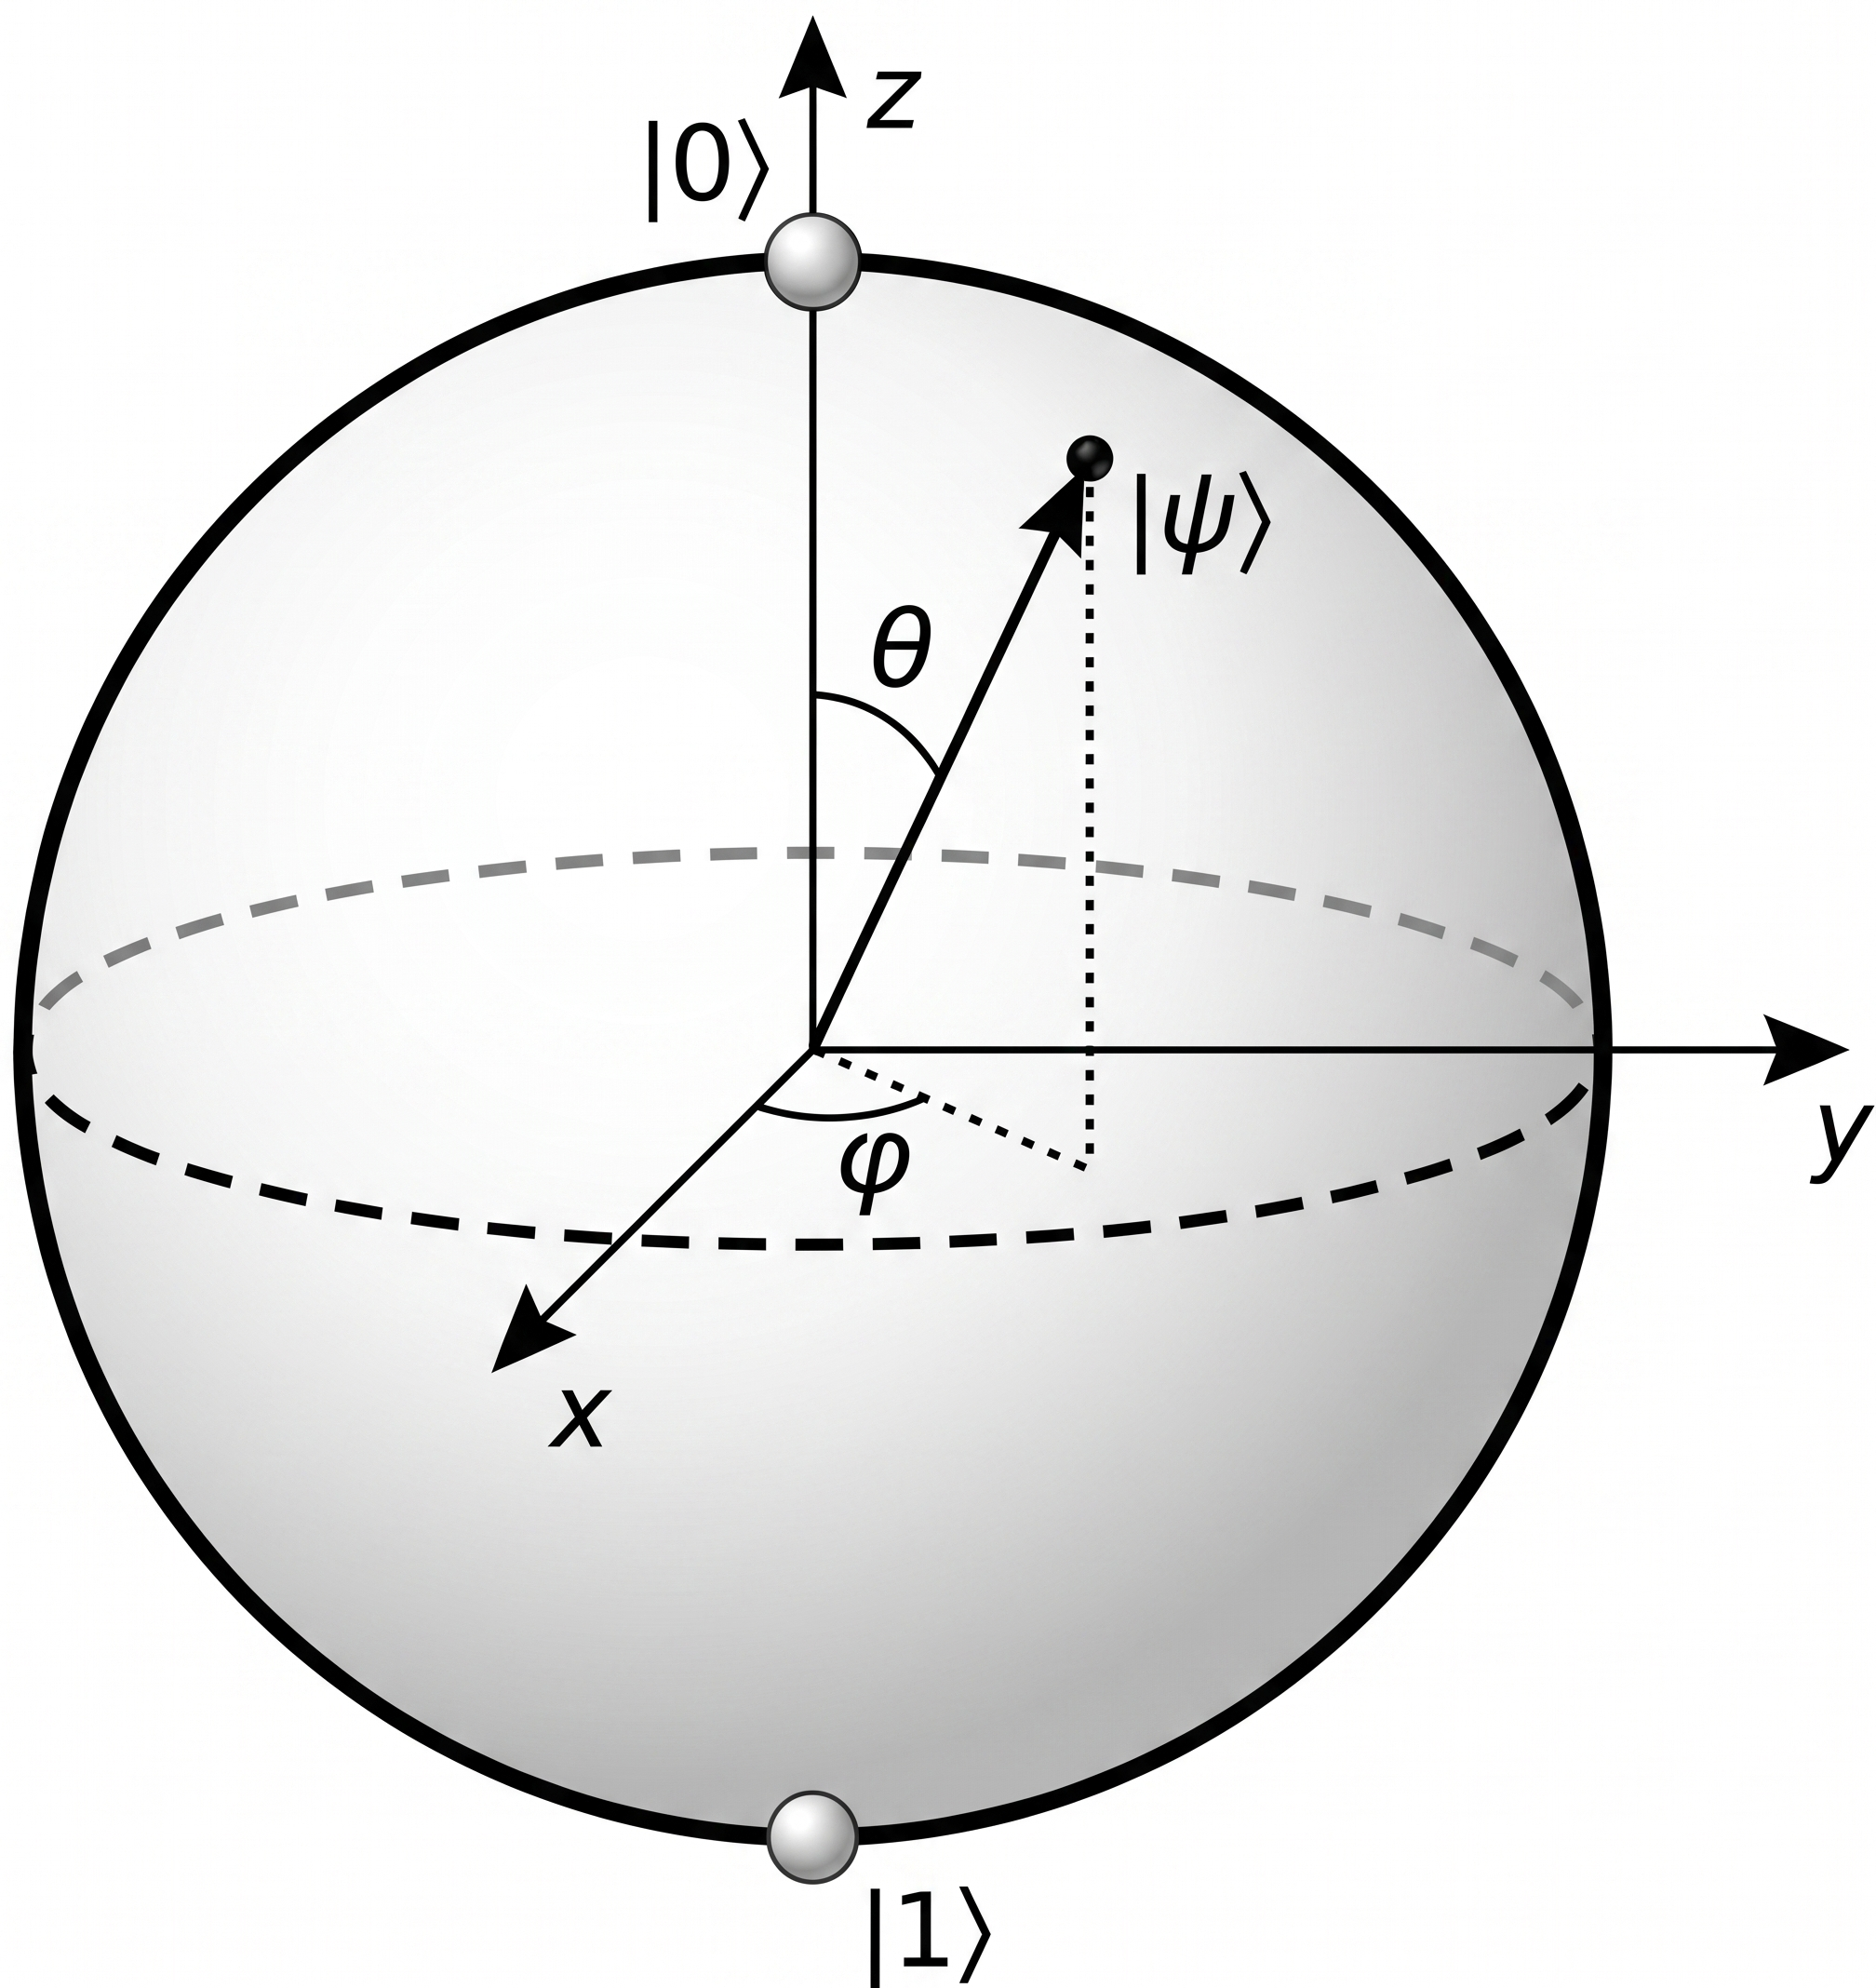
\includegraphics[width=0.5\textwidth]{assets/matcauBloch.png}
    \caption{Minh họa về mặt cầu Bloch.}
\end{figure}

Các điểm đặc biệt trên mặt cầu Bloch có thể được đọc trực tiếp từ phương trình
\eqref{eq:bloch-param} và dễ dàng xác định qua bảng sau:

\begin{table}[htbp]
\centering
\caption{Bảng trạng thái trên mặt cầu Bloch}
\renewcommand{\arraystretch}{1.4}
\begin{tabular}{lll}
\hline
Trạng thái & Tọa độ $(\theta, \phi)$ & Vị trí trên mặt cầu \\
\hline
$|0\rangle$ & $(0, \cdot)$ & Cực bắc \\
$|1\rangle$ & $(\pi, \cdot)$ & Cực nam \\
$|{+}\rangle$ & $(\pi/2, 0)$ & Xích đạo, hướng $+x$ \\
$|{-}\rangle$ & $(\pi/2, \pi)$ & Xích đạo, hướng $-x$ \\
$|{+i}\rangle = \frac{|0\rangle+i|1\rangle}{\sqrt{2}}$ & $(\pi/2, \pi/2)$ & Xích đạo, hướng $+y$\\
\hline
\end{tabular}
\label{tab:mat_cau_bloch}
\end{table}

\begin{remark}
Một đặc tính hình học quan trọng: hai trạng thái \emph{trực giao} về mặt đại số, tức là $\langle\phi|\psi\rangle = 0$ nhưng lại không vuông góc mà nằm ở \emph{hai cực
đối nhau} (\textit{antipodal}) trên mặt cầu Bloch. Chẳng hạn, $|0\rangle$ và
$|1\rangle$ nằm tại cực bắc và cực nam, còn $|+\rangle$ và $|-\rangle$ nằm đối
xứng qua tâm trên trục $x$. Điều này phản ánh thực tế rằng trong $\mathbb{C}^2$,
hai vectơ trực giao tạo thành góc $90°$ trong không gian Hilbert, nhưng biểu diễn
hình học trên mặt cầu Bloch bị ``kéo đôi" góc đó lên $180°$.
\end{remark}

Mặt cầu Bloch còn cung cấp diễn giải hình học tự nhiên cho các cổng lượng tử
đơn qubit. Có thể chứng minh rằng mọi toán tử unitary $U$ trên $\mathbb{C}^2$
đều có thể viết dưới dạng \cite{ref5}:
$$U = e^{-i\alpha\hat{n}\cdot\vec{\sigma}/2},$$
trong đó $\alpha \in \mathbb{R}$ là góc quay, $\hat{n}$ là vectơ đơn vị trong
$\mathbb{R}^3$ xác định trục quay, và $\vec{\sigma} = (\sigma_x, \sigma_y,
\sigma_z)$ là bộ ba ma trận $2\times 2$ được gọi là \textbf{ma trận Pauli} --
sẽ được định nghĩa tường minh ở mục 2.2. Biểu thức này có nghĩa là
mọi cổng lượng tử đơn qubit tương ứng với một \textbf{phép quay} vectơ Bloch
quanh trục $\hat{n}$ với góc $\alpha$ -- nhất quán với Tiên đề~2 rằng mọi tiến
hóa của hệ khép kín đều là unitary. Ví dụ đơn giản nhất: chọn $\hat{n} =
\hat{z}$ và $\alpha = \pi$, phép quay $180°$ quanh trục $z$ biến $|{+}\rangle$
tại xích đạo thành $|{-}\rangle$ -- giữ nguyên vĩ độ, đảo ngược kinh độ. Các
cổng cụ thể và phép quay Bloch tương ứng sẽ được phân tích đầy đủ ở mục 2.2.

% ---------------------------------------------------------------
\subsection*{Hệ nhiều qubit và tích tensor}

Khi mở rộng từ một qubit đơn lẻ sang hệ phức hợp, không gian trạng thái được
xây dựng bằng phép tích tensor (mục~\ref{subsec:tensor}) theo Tiên đề~4
(mục~\ref{sec:postulates}). Không gian trạng thái của hệ hai qubit là
$\mathbb{C}^2 \otimes \mathbb{C}^2$ -- không gian Hilbert bốn chiều với cơ sở
tính toán \cite{ref5}:
$$\{|00\rangle,\; |01\rangle,\; |10\rangle,\; |11\rangle\},$$
trong đó $|ab\rangle$ là ký hiệu tắt của $|a\rangle \otimes |b\rangle$.
Trạng thái tổng quát của hệ hai qubit là:
\begin{equation}
    |\psi\rangle = \alpha_{00}|00\rangle + \alpha_{01}|01\rangle
                + \alpha_{10}|10\rangle + \alpha_{11}|11\rangle,
    \quad \sum_{i,j}|\alpha_{ij}|^2 = 1.
    \label{eq:two-qubit}
\end{equation}

Tổng quát hóa lên hệ $n$ qubit, không gian trạng thái là $(\mathbb{C}^2)^{\otimes n}$
có số chiều $2^n$ -- tăng \emph{theo hàm mũ} với số qubit. Đây là nguồn gốc của
tính song song lượng tử: một trạng thái chồng chất đồng đều trên tất cả $2^n$ chuỗi
bit
\begin{equation}
    \frac{1}{\sqrt{2^n}}\sum_{x=0}^{2^n-1}|x\rangle
    \label{eq:uniform-superposition}
\end{equation}
mã hóa đồng thời $2^n$ giá trị đầu vào chỉ với $n$ qubit -- một bước khởi đầu trung
tâm trong thuật toán Deutsch--Jozsa.

\begin{example}[Trạng thái tích và trạng thái vướng víu]
Xét hai qubit, mỗi qubit ở trạng thái $|+\rangle = \frac{1}{\sqrt{2}}(|0\rangle
+ |1\rangle)$. Trạng thái của hệ là:
$$|{+}\rangle \otimes |{+}\rangle
= \frac{1}{2}(|00\rangle + |01\rangle + |10\rangle + |11\rangle).$$
Đây là \textbf{trạng thái tích} (\textit{product state}): có thể phân tách thành
tích của hai trạng thái qubit độc lập. Kết quả đo trên qubit thứ nhất không ảnh
hưởng đến phân bố xác suất của qubit thứ hai.

Ngược lại, trạng thái Bell
$$|\Phi^+\rangle = \frac{1}{\sqrt{2}}(|00\rangle + |11\rangle)$$
là \textbf{trạng thái vướng víu} (\textit{entangled state}): không thể viết dưới
dạng $|\psi_A\rangle \otimes |\psi_B\rangle$ cho bất kỳ $|\psi_A\rangle,
|\psi_B\rangle \in \mathbb{C}^2$ nào. Nếu đo qubit thứ nhất thu được $|0\rangle$,
qubit thứ hai lập tức suy sụp về $|0\rangle$ với xác suất $1$ -- bất kể khoảng
cách không gian giữa hai qubit.
\end{example}


\section{Cổng lượng tử một qubit và hai qubit}
\label{sec:gates}

Trong mô hình mạch lượng tử, sự tiến hóa của các trạng thái qubit được thực hiện thông qua các phép biến đổi tuyến tính bảo toàn chuẩn, gọi là \textbf{cổng lượng tử} (\textit{quantum gates}) \cite{ref5}. Khác với các cổng logic cổ điển như AND hay OR vốn không thuận nghịch, mọi cổng lượng tử đều được biểu diễn bằng một ma trận unitary và do đó luôn thuận nghịch. Cụ thể, cổng tác động lên hệ $n$ qubit được biểu diễn bằng một ma trận unitary kích thước $2^n \times 2^n$ thỏa mãn điều kiện $U^\dagger U = I$, trong đó $I$ là toán tử đồng nhất, và phép biến đổi ngược tương ứng với ma trận liên hợp Hermitian $U^\dagger$ của nó.

% ---------------------------------------------------------------
\subsection*{Ma trận Pauli và cổng Hadamard}

Bốn cổng một qubit cơ bản nhất là ma trận Pauli $X, Y, Z$ (hoặc $\sigma_1, \sigma_2, \sigma_3$) và cổng Hadamard $H$.
Cả bốn đều vừa là Hermitian vừa là unitary, tức $U^\dagger = U$ và $U^2 = I$
một tính chất đặc biệt không phải cổng nào cũng có \cite{ref5}.

\begin{definition}[Ma trận Pauli]
\label{def:pauli}
Ba \textbf{ma trận Pauli} là các toán tử một qubit được định nghĩa bởi:
$$X = \begin{pmatrix}0&1\\1&0\end{pmatrix}, \qquad
  Y = \begin{pmatrix}0&-i\\i&0\end{pmatrix}, \qquad
  Z = \begin{pmatrix}1&0\\0&-1\end{pmatrix}.$$
\end{definition}

\begin{proposition}[Tính chất đại số của ma trận Pauli]
\label{prop:pauli}
Các ma trận Pauli thỏa mãn:
\begin{enumerate}[label=(\roman*)]
    \item $X^2 = Y^2 = Z^2 = I$ \quad (tự nghịch đảo),
    \item $XY = iZ,\quad YZ = iX,\quad ZX = iY$ \quad (quan hệ giao hoán vòng),
    \item $XY = -YX,\quad YZ = -ZY,\quad ZX = -XZ$ \quad (phản giao hoán).
\end{enumerate}
\end{proposition}

Tác động của từng cổng Pauli lên cơ sở tính toán cho thấy vai trò hình học của
chúng trên mặt cầu Bloch \cite{ref5}:

\begin{example}[Tác động của các cổng Pauli]
\label{ex:pauli-action}
\textbf{Cổng $X$ -- lật bit lượng tử.} Cổng $X$ hoán vị hai trạng thái cơ sở:
$$X|0\rangle = |1\rangle, \qquad X|1\rangle = |0\rangle.$$
Với trạng thái tổng quát $|\psi\rangle = \alpha|0\rangle + \beta|1\rangle$:
$$X|\psi\rangle = \beta|0\rangle + \alpha|1\rangle.$$
Đây là phép quay góc $\pi$ quanh trục $x$ trên mặt cầu Bloch -- tương tự cổng
NOT cổ điển nhưng tác động lên biên độ phức.

\textbf{Cổng $Z$ -- lật pha.} Cổng $Z$ giữ nguyên $|0\rangle$ và đổi dấu $|1\rangle$:
$$Z|0\rangle = |0\rangle, \qquad Z|1\rangle = -|1\rangle.$$
Với trạng thái tổng quát:
$$Z|\psi\rangle = \alpha|0\rangle - \beta|1\rangle.$$
Không có tương đương cổ điển: $Z$ không thay đổi xác suất đo trong cơ sở tính
toán ($|\alpha|^2$ và $|\beta|^2$ giữ nguyên), nhưng thay đổi pha tương đối
và ảnh hưởng trực tiếp đến giao thoa. Trên mặt cầu
Bloch, đây là phép quay góc $\pi$ quanh trục $z$.

\textbf{Cổng $Y$.} Cổng $Y$ kết hợp cả lật bit lẫn lật pha:
$$Y|0\rangle = i|1\rangle, \qquad Y|1\rangle = -i|0\rangle,$$
tương ứng với phép quay góc $\pi$ quanh trục $y$ trên mặt cầu Bloch.
\end{example}

\begin{definition}[Cổng Hadamard]
\label{def:hadamard}
\textbf{Cổng Hadamard} $H$ được định nghĩa bởi:
$$H = \frac{1}{\sqrt{2}}\begin{pmatrix}1&1\\1&-1\end{pmatrix}.$$
\end{definition}

\begin{proposition}[Tính chất của cổng Hadamard]
\label{prop:hadamard}
Cổng Hadamard thỏa mãn $H^\dagger = H$ và $H^2 = I$. Tác động lên cơ sở tính
toán:
$$H|0\rangle = \frac{|0\rangle+|1\rangle}{\sqrt{2}} = |{+}\rangle, \qquad
  H|1\rangle = \frac{|0\rangle-|1\rangle}{\sqrt{2}} = |{-}\rangle,$$
và ngược lại $H|{+}\rangle = |0\rangle$, $H|{-}\rangle = |1\rangle$.
\end{proposition}

\begin{remark}
Cổng Hadamard là cổng trung tâm trong hầu hết các thuật toán lượng tử. Nó tạo ra
trạng thái chồng chất đồng đều từ trạng thái cơ sở -- bước khởi tạo bắt buộc
trong thuật toán Deutsch--Jozsa. Cụ thể, áp dụng $H^{\otimes n}$ lên
$|0\rangle^{\otimes n}$ tạo ra chồng chất đồng đều trên tất cả $2^n$ chuỗi bit, cho phép oracle $U_f$ xử lý toàn bộ đầu
vào trong một bước duy nhất (Khái niệm oracle $U_f$ sẽ được định nghĩa ở cuối mục 3.1 thuộc chương 3). Trên mặt cầu Bloch, $H$ tương ứng với phép quay góc
$\pi$ quanh trục $\hat{n} = \frac{1}{\sqrt{2}}(\hat{x}+\hat{z})$, biến cực bắc
$|0\rangle$ thành điểm xích đạo $|+\rangle$.
\end{remark}

% ---------------------------------------------------------------
\subsection*{Cổng pha $S$ và $T$}

Ngoài các cổng Pauli và Hadamard, hai cổng pha thường gặp trong tính toán lượng
tử là $S$ và $T$ \cite{ref5}:
$$S = \begin{pmatrix}1&0\\0&i\end{pmatrix}, \qquad
  T = \begin{pmatrix}1&0\\0&e^{i\pi/4}\end{pmatrix}.$$

\begin{remark}
Cả hai cổng đều giữ nguyên $|0\rangle$ và thêm một pha tương đối vào $|1\rangle$:
$S|1\rangle = i|1\rangle$ (quay góc $\frac{\pi}{2}$ quanh trục $z$) và
$T|1\rangle = e^{i\pi/4}|1\rangle$ (quay góc $\frac{\pi}{4}$ quanh trục $z$). Cần lưu ý
rằng $S = T^2$ và $Z = S^2 = T^4$, tức $Z$, $S$, $T$ là các phép quay quanh
cùng trục $z$ với góc lần lượt là $\pi$, $\frac{\pi}{2}$, $\frac{\pi}{4}$. Hai cổng này không
xuất hiện trực tiếp trong thuật toán Deutsch--Jozsa nhưng là thành phần cốt lõi
của bộ cổng phổ dụng được đề cập ở cuối mục này.
\end{remark}

% ---------------------------------------------------------------
\subsection*{Cổng CNOT, Toffoli và tính phổ dụng}

Các cổng một qubit không đủ để tạo ra sự vướng víu -- đặc tính phi cổ điển đòi
hỏi tương tác giữa nhiều qubit. Cổng hai qubit cơ bản nhất là
\textbf{CNOT} (\textit{Controlled-NOT}) \cite{ref5}.

\begin{definition}[Cổng CNOT]
\label{def:cnot}
Cổng \textbf{CNOT} tác động lên không gian $\mathbb{C}^2 \otimes \mathbb{C}^2$
với hai qubit đóng vai trò \emph{điều khiển} (\textit{control}) và \emph{đích}
(\textit{target}):
$$\mathrm{CNOT} =
\begin{pmatrix}1&0&0&0\\0&1&0&0\\0&0&0&1\\0&0&1&0\end{pmatrix},$$
tác động lên cơ sở tính toán theo quy tắc
$|c\rangle|t\rangle \mapsto |c\rangle|t \oplus c\rangle$,
trong đó $\oplus$ là phép cộng modulo $2$.
\end{definition}

\begin{example}[Tạo trạng thái Bell bằng CNOT]
\label{ex:bell}
Áp dụng $H$ lên qubit điều khiển rồi tác dụng CNOT:
$$|00\rangle \xrightarrow{H \otimes I}
  \frac{|0\rangle+|1\rangle}{\sqrt{2}}|0\rangle
  \xrightarrow{\mathrm{CNOT}}
  \frac{|00\rangle+|11\rangle}{\sqrt{2}} = |\Phi^+\rangle.$$
Trạng thái Bell $|\Phi^+\rangle$ là trạng thái vướng víu -- không thể phân tách
thành tích của hai trạng thái qubit độc lập (xem mục~\ref{sec:qubit}).
\end{example}

\begin{definition}[Cổng Toffoli]
\label{def:toffoli}
Cổng \textbf{Toffoli} (hay \textbf{CCNOT}) tác động lên không gian
$(\mathbb{C}^2)^{\otimes 3}$ với hai qubit điều khiển $c_1$, $c_2$ và một qubit
đích $t$:
$$\mathrm{Toffoli} =
\begin{pmatrix}
1&0&0&0&0&0&0&0\\
0&1&0&0&0&0&0&0\\
0&0&1&0&0&0&0&0\\
0&0&0&1&0&0&0&0\\
0&0&0&0&1&0&0&0\\
0&0&0&0&0&1&0&0\\
0&0&0&0&0&0&0&1\\
0&0&0&0&0&0&1&0
\end{pmatrix},$$
tác động lên cơ sở tính toán theo quy tắc
$$|c_1\rangle|c_2\rangle|t\rangle
  \mapsto |c_1\rangle|c_2\rangle|t \oplus (c_1 \wedge c_2)\rangle,$$
trong đó $\wedge$ là phép AND logic. Qubit đích bị lật khi và chỉ khi
\emph{cả hai} qubit điều khiển đều ở trạng thái $|1\rangle$; trong mọi trường
hợp còn lại, toàn bộ hệ giữ nguyên.
\end{definition}

\begin{remark}
Cổng Toffoli có ý nghĩa lý thuyết quan trọng vì quy tắc
$t \mapsto t \oplus (c_1 \wedge c_2)$ mô phỏng cổng AND cổ điển trong môi trường
\emph{khả nghịch}: chọn $t = 0$ thì qubit đích sau phép biến đổi chứa đúng giá
trị $c_1 \wedge c_2$, trong khi hai qubit điều khiển được bảo toàn nguyên vẹn.
Điều này là cơ sở để chứng minh mọi phép tính cổ điển đều có thể được mô phỏng
trên máy tính lượng tử.

Về \textbf{tính phổ dụng} (\textit{universality}): một bộ cổng được gọi là phổ
dụng nếu mọi toán tử unitary đều có thể xấp xỉ tùy ý chính xác bằng tổ hợp hữu
hạn các cổng trong bộ đó \cite{ref5}. Bộ $\{H, T, \mathrm{CNOT}\}$ là một bộ
cổng phổ dụng -- mọi thuật toán lượng tử đều có thể biên dịch về ba cổng này.
Đây là lý do $H$ và $T$ xuất hiện trong hầu hết các phân tích độ phức tạp mạch,
trong khi thuật toán Deutsch--Jozsa chỉ cần $H$ và $\mathrm{CNOT}$ (ẩn trong
cấu trúc oracle $U_f$) là đủ.
\end{remark}

\section{Mạch lượng tử: cấu trúc và phép đo}
\label{sec:circuit-measure}

Các cổng lượng tử đơn thuần mô tả từng phép biến đổi đơn lẻ. Để
thực hiện một thuật toán, các cổng đó cần được sắp xếp theo một trình tự xác định, đây là vai trò của \textbf{mạch lượng tử} (\textit{quantum circuit}). Mục này
trình bày cách đọc và phân tích mạch lượng tử, cơ chế phép đo kết thúc mạch, và
các tiêu chí đánh giá độ phức tạp -- ba công cụ cần thiết để theo dõi phân tích
thuật toán Deutsch--Jozsa.

% ---------------------------------------------------------------
\subsection*{Biểu đồ mạch và quy ước ký hiệu}

\begin{definition}[Mạch lượng tử]
\label{def:circuit}
Một \textbf{mạch lượng tử} trên $n$ qubit là một dãy hữu hạn các cổng lượng tử
$G_1, G_2, \dots, G_d$ tác động lần lượt lên các qubit của thanh ghi, kết thúc
bởi một hoặc nhiều phép đo \cite{ref5}. Toán tử unitary của toàn mạch là tích
có thứ tự:
$$U_{\mathrm{circuit}} = G_d \cdots G_2 G_1.$$
\end{definition}

Biểu đồ mạch là cách trực quan hóa định nghĩa trên theo quy ước sau \cite{ref5}:

\begin{convention}[Ký hiệu biểu đồ mạch]
\label{conv:circuit}
\hfill
\begin{enumerate}[label=(\roman*)]
    \item Mỗi \textbf{đường ngang} (dây) biểu diễn một qubit, thời gian chạy
          từ trái sang phải.
    \item Mỗi \textbf{hộp} trên dây biểu diễn một cổng, ký hiệu bằng tên cổng
          ($H$, $X$, $Z$, \ldots).
    \item \textbf{Cổng điều khiển} được ký hiệu bằng một điểm đặc $\bullet$ trên
          dây điều khiển, nối bằng đường thẳng đứng xuống cổng đích.
    \item \textbf{Phép đo} được ký hiệu bằng biểu tượng đồng hồ đo ở
          cuối dây, kèm đường đôi dẫn ra kết quả cổ điển.
    \item Trạng thái đầu vào của qubit thứ $k$ được ghi ở đầu dây tương ứng,
          thường là $|0\rangle$.
\end{enumerate}
Hình ảnh trực quan về ký hiệu mạch và dạng ma trận của các cổng lượng tử được trình bày ở Phụ lục 2.
\end{convention}

\begin{example}[Mạch tạo trạng thái Bell]
\label{ex:bell-circuit}
Mạch tạo trạng thái Bell $|\Phi^+\rangle$ được biểu diễn
như sau:


\begin{figure}[H]
    \centering
    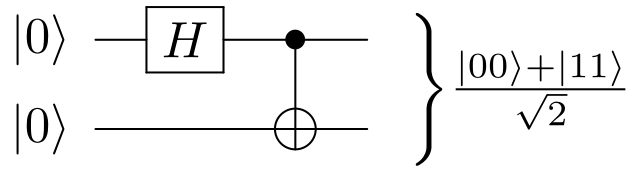
\includegraphics[width=0.8\textwidth]{assets/Bell-state.png}
    \caption{Mạch tạo trạng thái Bell.}
    \vspace{0.2cm}
    \small\textit{Nguồn: Wikipedia.}
\end{figure}

Đọc từ trái sang phải: cổng $H$ tác động lên qubit thứ nhất tạo trạng thái
$|+\rangle$, sau đó cổng CNOT với qubit thứ nhất làm điều khiển và qubit thứ
hai làm đích tạo ra vướng víu, cho kết quả
$|\Phi^+\rangle = \frac{1}{\sqrt{2}}(|00\rangle + |11\rangle)$.
\end{example}

\begin{remark}
Thứ tự nhân ma trận \emph{ngược} với thứ tự đọc trên biểu đồ: cổng xuất hiện
đầu tiên (trái nhất) trong biểu đồ tương ứng với toán tử đứng \emph{phải nhất}
trong tích ma trận. Trong Ví dụ~\ref{ex:bell-circuit}, toán tử toàn mạch là
$U = \mathrm{CNOT} \cdot (H \otimes I)$, không phải $(H \otimes I) \cdot
\mathrm{CNOT}$.
\end{remark}

% ---------------------------------------------------------------
\subsection*{Phép đo và sụp đổ trạng thái}

Phép đo kết thúc mạch lượng tử là ứng dụng trực tiếp của Tiên đề~3
(mục~\ref{sec:postulates}) vào thanh ghi qubit. Trong thực tế tính toán lượng
tử, phép đo hầu như luôn được thực hiện trong \textbf{cơ sở tính toán}
$\{|0\rangle, |1\rangle\}^{\otimes n}$ \cite{ref5}.

\begin{figure}[H]
    \centering
    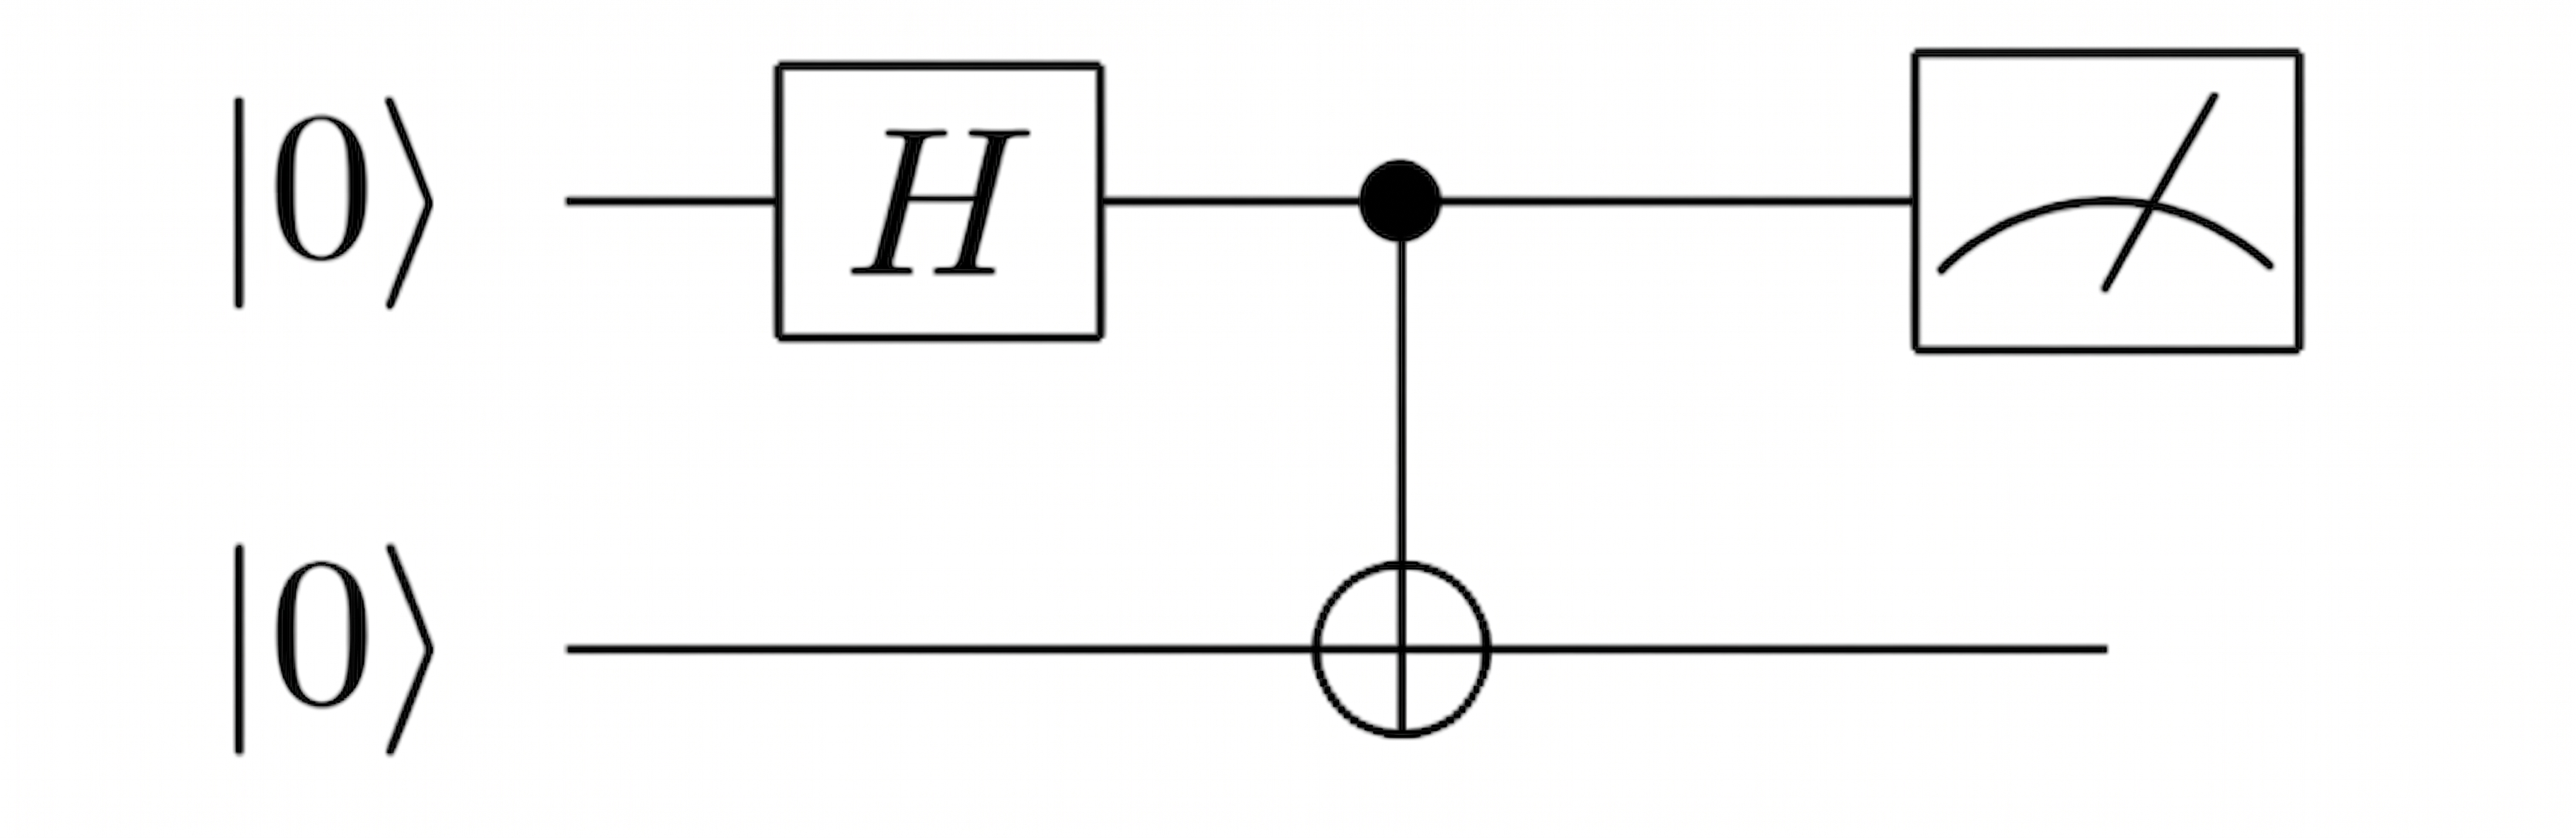
\includegraphics[width=0.8\textwidth]{assets/phepdo.png}
    \caption{Phép đo cho mạch tạo trạng thái Bell.}
\end{figure}

\begin{proposition}[Phép đo trong cơ sở tính toán]
\label{prop:measurement}
Cho hệ $n$ qubit ở trạng thái
$|\psi\rangle = \sum_{x \in \{0,1\}^n} \alpha_x |x\rangle$
với $\sum_x |\alpha_x|^2 = 1$. Khi đo toàn bộ thanh ghi trong cơ sở tính toán:
\begin{enumerate}[label=(\roman*)]
    \item Kết quả thu được là chuỗi bit $x \in \{0,1\}^n$ với xác suất
          $p(x) = |\alpha_x|^2$.
    \item Sau phép đo, trạng thái sụp đổ về $|x\rangle$ -- mọi thông tin về
          các biên độ khác bị xóa bỏ không thể phục hồi.
\end{enumerate}
\end{proposition}

\begin{remark}
Tính không khả nghịch của phép đo là điểm mấu chốt phân biệt mạch lượng tử với
các phép biến đổi unitary: trong khi mỗi cổng $U$ có thể đảo ngược bằng $U^\dagger$,
phép đo phá hủy thông tin về chồng chất và không có thao tác nào khôi phục lại
trạng thái trước đo. Vì lý do này, trong thiết kế mạch, phép đo \emph{luôn được
đặt ở cuối} sau tất cả các cổng unitary -- trừ các trường hợp đặc biệt như đo
giữa chừng trong tính toán có điều kiện.
\end{remark}


% ---------------------------------------------------------------
\subsection*{Độ phức tạp mạch: chiều sâu và số cổng}

Để so sánh hiệu quả của các thuật toán lượng tử, cần có tiêu chí định lượng mô
tả tài nguyên mà một mạch tiêu thụ. Hai tiêu chí phổ biến nhất là số cổng và
chiều sâu mạch \cite{ref5}.

\begin{definition}[Số cổng và chiều sâu mạch]
\label{def:complexity}
Cho mạch lượng tử $\mathcal{C}$:
\begin{enumerate}[label=(\roman*)]
    \item \textbf{Số cổng} (\textit{gate count}) là tổng số cổng trong mạch,
          đo lường tài nguyên tính toán tổng thể.
    \item \textbf{Chiều sâu} (\textit{circuit depth}) là số lớp cổng tối thiểu
          khi sắp xếp các cổng không tác động lên cùng qubit vào cùng một lớp --
          đo lường thời gian thực thi song song.
\end{enumerate}
\end{definition}

\begin{example}[Số cổng và chiều sâu của mạch Bell]
\label{ex:bell-complexity}
Mạch tạo trạng thái Bell ở Ví dụ~\ref{ex:bell-circuit} có:
\begin{itemize}
    \item Số cổng: $2$ (một cổng $H$ và một cổng CNOT).
    \item Chiều sâu: $2$ (cổng $H$ và CNOT không thể thực hiện song song vì
          CNOT phụ thuộc vào đầu ra của $H$).
\end{itemize}
\end{example}

\subsection*{Kết luận cuối Chương 2}
Chương này đã triển khai nền tảng toán học của Chương~1 thành mô hình
tính toán lượng tử cụ thể. Qubit được xác định là đơn vị thông tin cơ bản
với biểu diễn hình học trực quan trên mặt cầu Bloch; các cổng lượng tử
Pauli, Hadamard và CNOT được phân tích như các toán tử unitary tác động
lên trạng thái qubit; cấu trúc mạch và tiêu chí độ phức tạp cung cấp
ngôn ngữ để mô tả và đánh giá thuật toán.

\chapter{Thuật toán Deutsch-Jozsa: Lý thuyết và mô phỏng số}
Dựa trên nền tảng lý thuyết đã xây dựng, chương này tập trung phân tích thuật toán Deutsch--Jozsa~\cite{ref2} nhằm làm rõ ưu thế tuyệt đối của tính toán lượng tử so với máy tính cổ điển. Cấu trúc của chương gồm bốn phần: mục~\ref{sec:dj-problem} xây dựng bài toán và mô hình oracle; mục 3.2 phân tích toán học thuật toán; mục 3.3 định lượng ưu thế lượng tử; và mục 3.4 cuối cùng nhằm kiểm chứng lý thuyết qua mô phỏng số với Qiskit. Nội dung phân tích thuật toán trong chương được tham khảo từ các công trình đặt nền móng của Deutsch~\cite{ref1}, Deutsch \& Jozsa~\cite{ref2}, cùng với hệ thống tài liệu hướng dẫn lập trình và thực hành mạch lượng tử trực tuyến của thư viện Qiskit.
 
\section{Phát biểu bài toán và mô hình oracle lượng tử}
\label{sec:dj-problem}
 

Thuật toán Deutsch--Jozsa được xây dựng để giải một lớp bài toán cụ thể về hàm
boolean. Mục này lần lượt giới thiệu lớp bài toán đó, mô hình oracle lượng tử
mã hóa hàm vào mạch, và cơ chế phase kickback -- ba thành phần lý thuyết quan trọng để phân tích thuật toán.

%────────────────────────────────────────────────────────────────────────────
\subsection*{Hàm boolean: constant và balanced}
%────────────────────────────────────────────────────────────────────────────

\begin{definition}[Hàm boolean $n$ bit]
Cho $n \in \mathbb{N}^*$. Một \textbf{hàm boolean $n$ bit} là ánh xạ
$$f \colon \{0,1\}^n \longrightarrow \{0,1\}.$$
Miền xác định $\{0,1\}^n$ có $N = 2^n$ phần tử, mỗi phần tử là một chuỗi
nhị phân độ dài $n$.
\end{definition}

\begin{definition}[Hàm hằng và hàm cân bằng]
\label{def:const-balanced}
Hàm $f \colon \{0,1\}^n \to \{0,1\}$ được gọi là:
\begin{enumerate}[label=(\roman*)]
    \item \textbf{Hằng} (\textit{constant}) nếu $f(x) = c$ với mọi
          $x \in \{0,1\}^n$, trong đó $c \in \{0,1\}$ là một hằng số cố định;
    \item \textbf{Cân bằng} (\textit{balanced}) nếu $f$ nhận giá trị $0$ trên
          đúng một nửa miền xác định và giá trị $1$ trên nửa còn lại:
          $$\bigl|\{x \in \{0,1\}^n : f(x)=0\}\bigr|
            = \bigl|\{x \in \{0,1\}^n : f(x)=1\}\bigr| = 2^{n-1}.$$
\end{enumerate}
\end{definition}

\begin{example}[Minh họa với $n=2$]
\label{ex:const-balanced-n2}
Với $n=2$, miền xác định là $\{00, 01, 10, 11\}$ gồm $4$ phần tử.
\begin{itemize}
    \item Hàm hằng: $f_0(x) = 0$ với mọi $x$ (hoặc $f_1(x) = 1$ với mọi $x$).
    \item Hàm cân bằng: chẳng hạn $f(00)=f(01)=0$ và $f(10)=f(11)=1$ --
          đúng $2$ đầu vào cho ra $0$ và $2$ đầu vào cho ra $1$.
\end{itemize}

\end{example}

\begin{remark}
Hai lớp hàm hằng và cân bằng là rời nhau. Với $n \geq 1$, số hàm hằng luôn
là $2$, trong khi số hàm cân bằng là $\binom{2^n}{2^{n-1}}$, tăng rất nhanh
theo $n$. Chẳng hạn với $n=3$, có $\binom{8}{4} = 70$ hàm cân bằng nhưng
chỉ có $2$ hàm hằng.
\end{remark}

%────────────────────────────────────────────────────────────────────────────
\subsection*{Bài toán Deutsch ($n=1$) và tổng quát hóa $n$ bit}
%────────────────────────────────────────────────────────────────────────────

Năm 1985, D.\ Deutsch \cite{ref1} đặt ra câu hỏi: liệu một máy tính lượng tử
có thể xác định tính chất \emph{toàn cục} của một hàm boolean bằng ít lần truy
vấn hơn máy tính cổ điển không? Câu hỏi này dẫn đến phiên bản đơn giản nhất
của bài toán.

\begin{definition}[Bài toán Deutsch]
\label{def:deutsch-problem}
Cho một hàm $f \colon \{0,1\} \to \{0,1\}$ được cung cấp dưới dạng
\textbf{hộp đen} (\textit{black box}): chỉ có thể truy vấn giá trị $f(x)$ tại
các điểm $x$, không thể kiểm tra cấu trúc bên trong của $f$. Bài toán yêu cầu
xác định $f$ là hằng hay cân bằng.
\end{definition}

\begin{remark}
Với $n=1$, chỉ có bốn hàm boolean: hai hàm hằng ($f \equiv 0$ và $f \equiv 1$)
và hai hàm cân bằng ($f = \mathrm{id}$ tức $f(x)=x$, và $f = \mathrm{NOT}$ tức
$f(x)=1-x$). Một thuật toán cổ điển tất định cần tối thiểu $2$ lần truy vấn để
phân biệt hai lớp này -- vì một lần truy vấn duy nhất chỉ tiết lộ $f(0)$ hoặc
$f(1)$, không đủ để kết luận. Thuật toán Deutsch \cite{ref1} giải quyết bài toán
chỉ với \emph{một} lần truy vấn oracle lượng tử.
\end{remark}

Năm 1992, Deutsch và Jozsa \cite{ref2} tổng quát hóa bài toán lên $n$ bit tùy ý.

\begin{definition}[Bài toán Deutsch--Jozsa]
\label{def:dj-problem}
Cho $n \in \mathbb{N}^*$ và một hàm $f \colon \{0,1\}^n \to \{0,1\}$ được
\emph{đảm bảo} (\textit{promise}) thuộc một trong hai lớp hàm hằng hoặc hàm cân bằng. Bài toán yêu cầu xác định $f$ là hằng hay cân
bằng, với $f$ được truy cập thông qua một oracle lượng tử.
\end{definition}

\begin{remark}
Điều kiện ``được đảm bảo'' là bản chất của bài toán: không có giả thiết này,
không tồn tại thuật toán nào -- cổ điển hay lượng tử -- có thể đưa ra câu trả
lời đúng trong mọi trường hợp mà không truy vấn hết miền xác định. Trong trường
hợp cổ điển tất định, cần tối thiểu $2^{n-1}+1$ lần truy vấn để đảm bảo kết
quả chính xác \cite{ref5}: nếu $2^{n-1}$ lần truy vấn đầu cho cùng một giá trị,
$f$ vẫn có thể là hằng \emph{hoặc} cân bằng cho đến khi thực hiện thêm ít nhất
một lần truy vấn nữa. Thuật toán Deutsch--Jozsa giải quyết bài toán chỉ với
\emph{một} lần truy vấn oracle.
\end{remark}



%────────────────────────────────────────────────────────────────────────────
\subsection*{Toán tử oracle $U_f$ và phase kickback}
%────────────────────────────────────────────────────────────────────────────

Để tích hợp hàm $f$ vào mạch lượng tử, cần một biểu diễn toán tử unitary của
$f$. Theo Tiên đề~2 (mục~\ref{sec:postulates}), mọi phép biến đổi lượng tử đều
phải là unitary -- và do đó khả nghịch. Tuy nhiên, phần lớn các hàm boolean
không khả nghịch: nhiều đầu vào có thể cho cùng đầu ra, khiến không thể phục hồi
$x$ từ $f(x)$. Để giải quyết mâu thuẫn này, ta mở rộng không gian trạng thái
bằng cách thêm một \textbf{qubit phụ} (\textit{ancilla qubit}).

\begin{definition}[Oracle lượng tử $U_f$]
\label{def:oracle}
Cho $f \colon \{0,1\}^n \to \{0,1\}$. \textbf{Oracle lượng tử} $U_f$ là toán
tử unitary tác động trên không gian $(\mathbb{C}^2)^{\otimes n} \otimes
\mathbb{C}^2$ theo quy tắc:
$$U_f \colon |x\rangle|y\rangle \;\longmapsto\; |x\rangle|y \oplus f(x)\rangle,$$
trong đó $x \in \{0,1\}^n$, $y \in \{0,1\}$, và $\oplus$ là phép cộng modulo $2$.
Thanh ghi $|x\rangle$ ($n$ qubit) được gọi là \textbf{thanh ghi vào}; qubit
$|y\rangle$ được gọi là \textbf{qubit đích} (\textit{target qubit}).
\end{definition}


\begin{figure}[H]
    \centering
    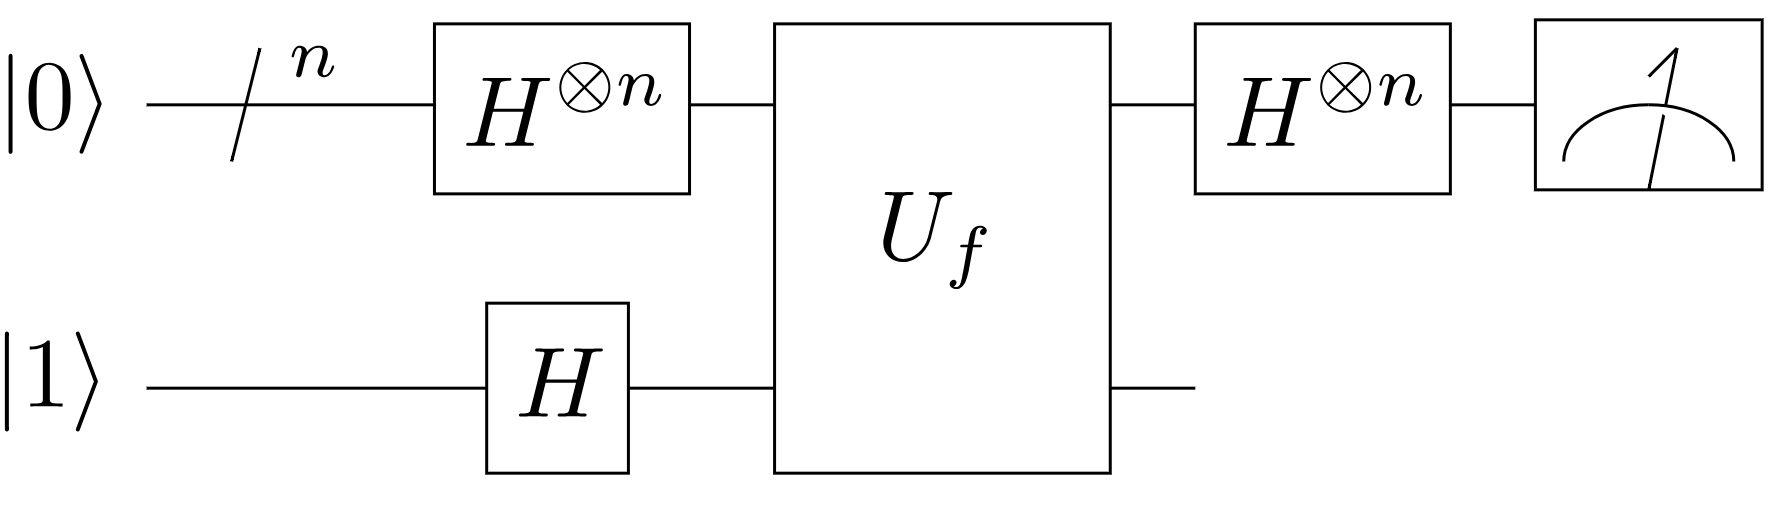
\includegraphics[width=0.8\textwidth]{assets/machDJ.png}
    \caption{Minh họa biểu đồ có chứa mạch oracle $U_f$.}
\end{figure}

\begin{proposition}
\label{prop:uf-unitary}
Toán tử $U_f$ là toán tử unitary và tự nghịch đảo ($U_f^2 = I$).
\end{proposition}

\begin{proof}
$U_f$ hoán vị các phần tử của cơ sở tính toán $\{|x\rangle|y\rangle\}$ vì với
mọi $x, y$: $y \oplus f(x) \oplus f(x) = y$. Hoán vị bảo toàn tích trong nên
$U_f$ là unitary. Áp dụng $U_f$ hai lần:
$$U_f^2|x\rangle|y\rangle
= U_f|x\rangle|y \oplus f(x)\rangle
= |x\rangle|y \oplus f(x) \oplus f(x)\rangle
= |x\rangle|y\rangle.$$
Vậy $U_f^2 = I$, tức $U_f^{-1} = U_f = U_f^\dagger$.
\end{proof}

\begin{remark}
Tính chất $U_f^2 = I$ -- tự nghịch đảo -- là hệ quả trực tiếp của phép cộng
modulo $2$: áp dụng oracle hai lần khôi phục lại trạng thái ban đầu. Đây cũng
là lý do thiết kế oracle theo cấu trúc $|x\rangle|y \oplus f(x)\rangle$ thay vì
lưu trực tiếp $f(x)$ vào một qubit: cấu trúc này đảm bảo tính khả nghịch mà
không cần thêm bước xóa bộ nhớ.
\end{remark}

Cơ chế quan trọng nhất quyết định hiệu quả của thuật toán là \textbf{phase
kickback}: thay vì đọc kết quả từ qubit đích, ta chuẩn bị qubit đích ở trạng
thái đặc biệt sao cho thông tin về $f(x)$ được ``đẩy ngược'' vào pha của thanh
ghi vào.

\begin{proposition}[Phase kickback]
\label{prop:phase-kickback}
Nếu qubit đích được chuẩn bị ở trạng thái
$|{-}\rangle = \dfrac{|0\rangle - |1\rangle}{\sqrt{2}}$, thì:
$$U_f\bigl(|x\rangle \otimes |{-}\rangle\bigr)
= (-1)^{f(x)}\,|x\rangle \otimes |{-}\rangle.$$
\end{proposition}

\begin{proof}
Khai triển $|{-}\rangle$ và áp dụng tuyến tính:
\begin{align*}
U_f\!\left(|x\rangle \otimes \frac{|0\rangle - |1\rangle}{\sqrt{2}}\right)
&= \frac{1}{\sqrt{2}}\Bigl(
    U_f|x\rangle|0\rangle - U_f|x\rangle|1\rangle
  \Bigr) \\
&= \frac{1}{\sqrt{2}}\Bigl(
    |x\rangle|f(x)\rangle - |x\rangle|1 \oplus f(x)\rangle
  \Bigr).
\end{align*}

\noindent\textbf{Trường hợp $f(x)=0$:}
$$= \frac{1}{\sqrt{2}}\bigl(|x\rangle|0\rangle - |x\rangle|1\rangle\bigr)
= |x\rangle \otimes |{-}\rangle = (-1)^0\,|x\rangle \otimes |{-}\rangle.$$

\noindent\textbf{Trường hợp $f(x)=1$:}
$$= \frac{1}{\sqrt{2}}\bigl(|x\rangle|1\rangle - |x\rangle|0\rangle\bigr)
= -|x\rangle \otimes |{-}\rangle = (-1)^1\,|x\rangle \otimes |{-}\rangle.$$

Gộp hai trường hợp: $U_f(|x\rangle \otimes |{-}\rangle)
= (-1)^{f(x)}|x\rangle \otimes |{-}\rangle$.
\end{proof}

\begin{remark}
Mệnh đề~\ref{prop:phase-kickback} có ba hệ quả quan trọng cần lưu ý.

\textbf{Thứ nhất}, qubit đích \emph{không thay đổi} sau tác động của $U_f$: nó
vẫn ở trạng thái $|{-}\rangle$ bất kể giá trị $f(x)$. Điều này giải thích tên
gọi ``phase kickback'': pha $(-1)^{f(x)}$ bị ``đá ngược'' từ qubit đích lên
thanh ghi vào, thay vì lưu lại ở qubit đích.

\textbf{Thứ hai}, pha $(-1)^{f(x)}$ là pha \emph{toàn cục} khi xét trên một
trạng thái đơn lẻ $|x\rangle$ -- không thể đo trực tiếp. Tuy nhiên, khi thanh ghi vào ở trạng thái
\emph{chồng chất} $\sum_x \alpha_x|x\rangle$, pha $(-1)^{f(x)}$ trở thành pha
\emph{tương đối} giữa các số hạng -- và do đó có thể quan sát được qua giao
thoa lượng tử.

\textbf{Thứ ba}, đây là lý do qubit đích được gọi là \emph{qubit phụ} theo
nghĩa chức năng: sau khi đóng vai trò trung gian truyền thông tin từ pha
thanh ghi vào, nó không tham gia vào phép đo cuối mạch.
\end{remark}

\begin{remark}
Cơ chế phase kickback không đặc thù cho thuật toán Deutsch--Jozsa mà là một
kỹ thuật tổng quát, xuất hiện trong nhiều thuật toán lượng tử quan trọng như
thuật toán Grover (tìm kiếm) và thuật toán Shor (phân tích nhân tử). Nielsen
và Chuang \cite{ref5} coi đây là một trong những kỹ thuật nền tảng của lập
trình lượng tử.
\end{remark}



\section{Phân tích toán học từng bước thuật toán}
Mục này trình bày phân tích toán học đầy đủ thuật toán Deutsch--Jozsa cho hàm
$f:\{0,1\}^n \to \{0,1\}$, theo từng bước biến đổi trạng thái bằng ký hiệu
Dirac. Ký hiệu $|x\rangle$ với $x \in \{0,1\}^n$ chỉ trạng thái cơ sở tính
toán của $n$ qubit đầu vào, và phép đo ở bước cuối được phân tích theo Tiên
đề~3 (mục~\ref{sec:postulates}).
 
% ---------------------------------------------------------------
\subsection*{Bước 1: Chuẩn bị trạng thái ban đầu}
 
Hệ gồm $n+1$ qubit được khởi tạo ở trạng thái:
\begin{equation}
    |\psi_0\rangle = |0\rangle^{\otimes n}|1\rangle.
    \label{eq:dj-init}
\end{equation}
$n$ qubit đầu tiên (thanh ghi đầu vào) ở trạng thái $|0\rangle^{\otimes n}$,
qubit thứ $(n+1)$ (qubit bổ trợ, \textit{ancilla}) ở trạng thái $|1\rangle$.
Việc chọn $|1\rangle$ cho qubit bổ trợ -- thay vì $|0\rangle$ -- là điều kiện
cần thiết để cơ chế \textit{phase kickback} hoạt động ở Bước~3, như sẽ thấy
rõ bên dưới.
 
% ---------------------------------------------------------------
\subsection*{Bước 2: Biến đổi Hadamard $H^{\otimes(n+1)}$}
 
Áp dụng cổng Hadamard đồng thời lên tất cả $n+1$ qubit. Sử dụng kết quả
$H|0\rangle = |{+}\rangle$ và $H|1\rangle = |{-}\rangle$,
trạng thái sau biến đổi là:
\begin{equation}
    |\psi_1\rangle
    = H^{\otimes n}|0\rangle^{\otimes n} \otimes H|1\rangle
    = \frac{1}{\sqrt{2^n}}\sum_{x=0}^{2^n-1}|x\rangle
      \otimes \frac{|0\rangle - |1\rangle}{\sqrt{2}}.
    \label{eq:dj-hadamard1}
\end{equation}
Thanh ghi đầu vào đạt trạng thái chồng chất đồng đều trên tất cả $2^n$ chuỗi
bit -- đây là biểu thức~\eqref{eq:uniform-superposition} đã giới thiệu ở
mục~\ref{sec:qubit}. Qubit bổ trợ ở trạng thái $|{-}\rangle =
\frac{|0\rangle-|1\rangle}{\sqrt{2}}$, trạng thái sẽ hấp thụ thông tin về
$f$ dưới dạng pha ở bước tiếp theo.
 
% ---------------------------------------------------------------
\subsection*{Bước 3 \quad Áp dụng oracle $U_f$ và phase kickback}
 
Oracle $U_f$ tác động lên toàn hệ theo quy tắc
$U_f|x\rangle|y\rangle = |x\rangle|y \oplus f(x)\rangle$. Tác động lên từng hạng tử của~\eqref{eq:dj-hadamard1},
xét riêng qubit bổ trợ ở trạng thái $\frac{|0\rangle-|1\rangle}{\sqrt{2}}$:
 
\begin{itemize}
    \item Nếu $f(x) = 0$: $U_f|x\rangle\frac{|0\rangle-|1\rangle}{\sqrt{2}}
          = |x\rangle\frac{|0\rangle-|1\rangle}{\sqrt{2}}
          = (+1)\cdot|x\rangle\frac{|0\rangle-|1\rangle}{\sqrt{2}}.$
    \item Nếu $f(x) = 1$: $U_f|x\rangle\frac{|0\rangle-|1\rangle}{\sqrt{2}}
          = |x\rangle\frac{|1\rangle-|0\rangle}{\sqrt{2}}
          = (-1)\cdot|x\rangle\frac{|0\rangle-|1\rangle}{\sqrt{2}}.$
\end{itemize}
 
Trong cả hai trường hợp, qubit bổ trợ \emph{trở lại} trạng thái
$\frac{|0\rangle-|1\rangle}{\sqrt{2}}$ (không bị thay đổi), còn toàn bộ thông
tin về $f(x)$ được \emph{đẩy ngược} vào pha của thanh ghi đầu vào dưới dạng
hệ số $(-1)^{f(x)}$ -- đây chính là cơ chế \textbf{phase kickback}. Hai trường
hợp gộp lại thành:
\begin{equation}
    U_f\left(|x\rangle\frac{|0\rangle-|1\rangle}{\sqrt{2}}\right)
    = (-1)^{f(x)}|x\rangle\frac{|0\rangle-|1\rangle}{\sqrt{2}}.
    \label{eq:kickback}
\end{equation}
Áp dụng~\eqref{eq:kickback} cho toàn bộ trạng thái~\eqref{eq:dj-hadamard1},
qubit bổ trợ tách ra như một thừa số chung và từ đây có thể bỏ qua:
\begin{equation}
    |\psi_2\rangle
    = \frac{1}{\sqrt{2^n}}\sum_{x=0}^{2^n-1}(-1)^{f(x)}|x\rangle
      \otimes \frac{|0\rangle-|1\rangle}{\sqrt{2}}.
    \label{eq:dj-after-oracle}
\end{equation}
 
% ---------------------------------------------------------------
\subsection*{Bước 4 \quad Hadamard lần hai và xác suất đo}
 
\subsubsection*{Biến đổi Hadamard lần hai}
 
Áp dụng $H^{\otimes n}$ lên thanh ghi đầu vào. Sử dụng công thức tổng quát
của biến đổi Hadamard trên $n$ qubit \cite{ref5}:
\begin{equation}
    H^{\otimes n}|x\rangle
    = \frac{1}{\sqrt{2^n}}\sum_{z=0}^{2^n-1}(-1)^{x\cdot z}|z\rangle,
    \label{eq:hadamard-general}
\end{equation}
trong đó $x \cdot z = \sum_{k=1}^{n} x_k z_k \pmod{2}$ là tích vô hướng bit.
Thay~\eqref{eq:hadamard-general} vào~\eqref{eq:dj-after-oracle}:
\begin{align}
    |\psi_3\rangle
    &= \frac{1}{\sqrt{2^n}}\sum_{x=0}^{2^n-1}(-1)^{f(x)}
       \cdot\frac{1}{\sqrt{2^n}}\sum_{z=0}^{2^n-1}(-1)^{x\cdot z}|z\rangle
       \notag\\
    &= \sum_{z=0}^{2^n-1}
       \left(\frac{1}{2^n}\sum_{x=0}^{2^n-1}(-1)^{f(x)+x\cdot z}\right)|z\rangle.
    \label{eq:dj-final}
\end{align}
 
\subsubsection*{Tính xác suất đo trạng thái $|0\rangle^{\otimes n}$}
 
Theo Hệ quả~\ref{cor:born} (Quy tắc Born), biên độ xác suất đo được
$|0\rangle^{\otimes n}$ (tức $z = 0$) là hệ số đứng trước $|0\rangle^{\otimes n}$
trong~\eqref{eq:dj-final}:
\begin{equation}
    A_0 = \frac{1}{2^n}\sum_{x=0}^{2^n-1}(-1)^{f(x)},
    \label{eq:amplitude-zero}
\end{equation}
và xác suất đo được $|0\rangle^{\otimes n}$ là $p(0^n) = |A_0|^2$.
 
\begin{proposition}[Tiêu chuẩn phân loại Deutsch--Jozsa]
\label{prop:dj-criterion}
Với hàm $f:\{0,1\}^n\to\{0,1\}$ là hằng số hoặc cân bằng:
\begin{enumerate}[label=(\roman*)]
    \item Nếu $f$ \textbf{hằng số}: $f(x) = c$ với mọi $x$, nên
          $(-1)^{f(x)} = (-1)^c = \pm 1$ không đổi. Tổng~\eqref{eq:amplitude-zero}
          là $2^n$ số hạng cùng dấu:
          $$A_0 = \frac{1}{2^n}\cdot 2^n\cdot(\pm 1) = \pm 1,$$
          do đó $p(0^n) = |A_0|^2 = 1$. Phép đo \emph{luôn} cho kết quả
          $|0\rangle^{\otimes n}$.
    \item Nếu $f$ \textbf{cân bằng}: đúng $2^{n-1}$ giá trị $x$ cho
          $(-1)^{f(x)} = +1$ và $2^{n-1}$ giá trị cho $(-1)^{f(x)} = -1$,
          các số hạng triệt tiêu nhau hoàn toàn:
          $$A_0 = \frac{1}{2^n}\cdot(2^{n-1} - 2^{n-1}) = 0,$$
          do đó $p(0^n) = 0$. Phép đo \emph{không bao giờ} cho kết quả
          $|0\rangle^{\otimes n}$.
\end{enumerate}
\end{proposition}
 
\begin{remark}
Mệnh đề~\ref{prop:dj-criterion} cho thấy hai trường hợp hoàn toàn phân biệt
nhau: xác suất nhận giá trị $1$ hoặc $0$, không có vùng trung gian. Vì vậy,
\emph{một lần} áp dụng oracle và một lần đo là đủ để kết luận chắc chắn.
Cơ chế nền tảng là giao thoa lượng tử: ở trường hợp hằng số, các biên độ cùng
pha tăng cường lẫn nhau và tập trung hoàn toàn vào $|0\rangle^{\otimes n}$; ở
trường hợp cân bằng, các biên độ ngược pha triệt tiêu nhau hoàn toàn tại cùng
trạng thái đó.
\end{remark}

\section{Ưu thế lượng tử: $O(1)$ vs $O(2^{n-1})$}
Mục này phân tích ưu thế của thuật toán Deutsch--Jozsa so với mọi thuật toán
cổ điển tất định, phân tích vai trò của giao thoa lượng tử như cơ chế nền tảng
tạo ra ưu thế đó, và thảo luận về giới hạn cũng như ý nghĩa thực tiễn của kết
quả.
 
% ---------------------------------------------------------------
\subsection*{So sánh độ phức tạp}
 
\subsubsection*{Thuật toán lượng tử: $O(1)$ lần truy vấn oracle}
 
Toàn bộ thuật toán Deutsch--Jozsa
thực hiện đúng \textbf{một lần} truy vấn oracle $U_f$ và cho kết quả chắc chắn:
phép đo thanh ghi đầu vào sau Hadamard lần hai luôn ra $|0\rangle^{\otimes n}$
nếu $f$ hằng số, và không bao giờ ra $|0\rangle^{\otimes n}$ nếu $f$ cân bằng
(Mệnh đề~\ref{prop:dj-criterion}). Độ phức tạp truy vấn là:
\begin{equation}
    Q_{\text{lượng tử}} = 1 = O(1).
    \label{eq:quantum-complexity}
\end{equation}
 
\subsubsection*{Thuật toán cổ điển tất định: $O(2^{n-1}+1)$ lần truy vấn}
 
Một thuật toán cổ điển \emph{tất định} (\textit{deterministic}) phải truy vấn
$f$ tuần tự tại các điểm $x_1, x_2, \ldots$ cho đến khi có thể kết luận chắc
chắn. Trong trường hợp xấu nhất:
 
\begin{itemize}
    \item Sau $k < 2^{n-1}+1$ lần truy vấn, nếu tất cả đều cho cùng kết quả
          (ví dụ đều bằng $0$), thuật toán chưa thể phân biệt: $f$ có thể là
          hằng số $0$, hoặc là hàm cân bằng với đúng $2^{n-1}$ giá trị $0$ và
          $2^{n-1}$ giá trị $1$ (trong đó các điểm chưa được truy vấn đều là $1$).
    \item Chỉ sau khi truy vấn $2^{n-1}+1$ điểm và nhận được cùng kết quả, thuật
          toán mới có thể kết luận $f$ là hằng số -- vì một hàm cân bằng không
          thể có nhiều hơn $2^{n-1}$ điểm cùng giá trị.
\end{itemize}
 
Do đó độ phức tạp truy vấn trong trường hợp xấu nhất là:
\begin{equation}
    Q_{\text{cổ điển}} = 2^{n-1} + 1 = O(2^n).
    \label{eq:classical-complexity}
\end{equation}
 
\begin{remark}
Cần phân biệt \emph{độ phức tạp truy vấn} (số lần gọi oracle) và \emph{độ phức
tạp thời gian} (số cổng lượng tử). Về độ phức tạp thời gian, thuật toán
Deutsch--Jozsa cần $O(n)$ cổng Hadamard và một lần áp dụng $U_f$ -- hiệu quả
hơn đáng kể so với $O(2^n)$ bước của thuật toán cổ điển, nhưng so sánh chính
xác phụ thuộc vào cách triển khai oracle $U_f$ trên phần cứng cụ thể.
\end{remark}
 
% ---------------------------------------------------------------
\subsection*{Vai trò của giao thoa lượng tử}
 
Ưu thế $O(1)$ không đến từ tính song song lượng tử đơn thuần -- sự chồng chất
$\frac{1}{\sqrt{2^n}}\sum_x |x\rangle$ mã hóa $2^n$ đầu vào đồng thời, nhưng
phép đo ngẫu nhiên trên trạng thái này chỉ trả về một giá trị duy nhất. Ưu thế
thực sự đến từ \textbf{giao thoa lượng tử} như một cơ chế kiểm soát có chọn
lọc phân bố xác suất.
 
Nhìn lại biên độ xác suất~\eqref{eq:amplitude-zero}:
$$A_0 = \frac{1}{2^n}\sum_{x=0}^{2^n-1}(-1)^{f(x)}.$$
Đây là \emph{tổng giao thoa} của $2^n$ biên độ phức, mỗi biên độ mang pha
$(-1)^{f(x)} \in \{+1, -1\}$:
 
\begin{itemize}
    \item \textbf{Hàm hằng số -- giao thoa tăng cường:} mọi số hạng cùng dấu,
          tổng đạt giá trị cực đại $|A_0| = 1$. Toàn bộ xác suất tập trung vào
          $|0\rangle^{\otimes n}$.
    \item \textbf{Hàm cân bằng -- giao thoa triệt tiêu:} số hạng $+1$ và $-1$
          bằng nhau, tổng triệt tiêu hoàn toàn $A_0 = 0$. Xác suất đo được
          $|0\rangle^{\otimes n}$ bằng không.
\end{itemize}
 
Hai trường hợp được thiết kế để phân biệt nhau \emph{hoàn toàn} tại một điểm
duy nhất trong không gian kết quả đo -- đây là lý do một phép đo là đủ.
 
% ---------------------------------------------------------------
\subsection*{Giới hạn và ý nghĩa thực tiễn}
 
\subsubsection*{Giới hạn của bài toán}
 
Ưu thế mũ của thuật toán Deutsch--Jozsa được xây dựng trên một \textbf{giả
thiết mạnh}: đầu vào được đảm bảo là hằng số hoặc cân bằng -- không có trường
hợp nào khác. Trong thực tế, hàm $f$ tùy ý có thể không thỏa mãn điều kiện
này, và thuật toán không cung cấp cơ chế xử lý trường hợp trung gian.
 
Ngoài ra, nếu cho phép thuật toán cổ điển sử dụng \textbf{ngẫu nhiên}
(\textit{randomized algorithm}), khoảng cách về độ phức tạp thu hẹp đáng kể:
chỉ cần truy vấn $O(1)$ điểm ngẫu nhiên, thuật toán cổ điển ngẫu nhiên có thể
kết luận đúng với xác suất tùy ý gần $1$ \cite{ref5}. Cụ thể, nếu truy vấn $k$
điểm ngẫu nhiên và nhận được cùng kết quả, xác suất kết luận sai (tức $f$ thực
ra là cân bằng) không vượt quá $2^{1-k}$. Với $k = 30$, xác suất sai nhỏ hơn
$10^{-9}$ -- đủ cho hầu hết ứng dụng thực tế. Như vậy, ưu thế \emph{mũ tuyệt
đối} của thuật toán Deutsch--Jozsa chỉ tồn tại so với \emph{thuật toán cổ điển
tất định}, không phải so với thuật toán ngẫu nhiên.
 
\subsubsection*{Ý nghĩa lý thuyết}
 
Dù có giới hạn thực tiễn, thuật toán Deutsch--Jozsa mang ý nghĩa lý thuyết nền
tảng theo ba phương diện:
 
\begin{enumerate}
    \item \textbf{Bằng chứng đầu tiên về ưu thế lượng tử tất định.} Đây là
          thuật toán lượng tử đầu tiên được chứng minh \emph{chắc chắn} (không
          phải xác suất) nhanh hơn mọi thuật toán cổ điển tất định tương đương
          \cite{ref3}. Kết quả này thiết lập nguyên tắc rằng máy tính lượng tử
          có thể vượt trội máy tính cổ điển về mặt lý thuyết.
    \item \textbf{Mô hình thiết kế thuật toán lượng tử.} Cấu trúc
          khởi tạo $\to$ Hadamard $\to$ oracle $\to$ Hadamard $\to$ đo là mẫu
          thiết kế xuất hiện lại trong nhiều thuật toán lượng tử quan trọng hơn,
          bao gồm thuật toán Simon, biến đổi Fourier lượng tử, và thuật toán
          Shor \cite{ref5}.
    \item \textbf{Minh họa nguyên lý giao thoa có kiểm soát.} Thuật toán cho
          thấy rằng giá trị của tính toán lượng tử không nằm ở việc \emph{thử
          song song} $2^n$ đầu vào, mà ở việc \emph{thiết kế giao thoa} sao
          cho kết quả mong muốn được khuếch đại và kết quả không mong muốn bị
          triệt tiêu -- nguyên lý cốt lõi của hầu hết thuật toán lượng tử hiệu
          quả đã biết.
\end{enumerate}

\section{Triển khai mô phỏng với Qiskit}
\label{sec:qiskit}

Phần lý thuyết ở các mục trước đã chứng minh chặt chẽ rằng thuật toán
Deutsch--Jozsa cho kết quả đúng với xác suất $1$ trong một lần truy vấn
oracle duy nhất. Mục này hiện thực hóa
và kiểm chứng kết quả đó bằng mô phỏng số trên nền tảng Qiskit, với
$n = 1, 2, 3, 4, 5$ qubit đầu vào.

%────────────────────────────────────────────────────────────────────────────
\subsection*{Môi trường và cấu hình}
%────────────────────────────────────────────────────────────────────────────

Toàn bộ mô phỏng được thực hiện trên môi trường Python với các thư viện
chính như sau:

\begin{table}[htbp]
\centering
\caption{Môi trường phần mềm cho mô phỏng}
\label{tab:env}
\begin{tabular}{ll}
\hline
\textbf{Thành phần} & \textbf{Phiên bản} \\
\hline
Python        & 3.10 \\
Qiskit        & 1.0  \\
qiskit-aer    & 0.13 \\
NumPy         & 1.26 \\
Matplotlib    & 3.8  \\
\hline
\end{tabular}

\end{table}

Bộ mô phỏng được sử dụng là \texttt{StatevectorSimulator} của Qiskit Aer.
Toàn bộ mã nguồn được công bố trong
Phụ lục 1.

%────────────────────────────────────────────────────────────────────────────
\subsection*{Xây dựng oracle: constant và balanced}
%────────────────────────────────────────────────────────────────────────────

Để mô phỏng, cần xây dựng tường minh hai loại oracle $U_f$ tương ứng với
hàm hằng và hàm cân bằng.

\textbf{Oracle hằng.} Với hàm hằng $f \equiv c$, oracle $U_f$ tác động theo
$|x\rangle|y\rangle \mapsto |x\rangle|y \oplus c\rangle$. Điều này có nghĩa:
\begin{itemize}
    \item $f \equiv 0$: oracle là toán tử đồng nhất $I$ -- không tác động
          lên qubit nào.
    \item $f \equiv 1$: oracle chỉ áp dụng cổng $X$ lên qubit đích, độc lập
          với mọi qubit đầu vào.
\end{itemize}
Cả hai trường hợp đều không tạo ra sự vướng víu giữa thanh ghi vào và
qubit đích.

\textbf{Oracle cân bằng.} Với hàm cân bằng, chọn một chuỗi nhị phân $s \in \{0,1\}^n$ bất kỳ (không phải chuỗi
toàn $0$), đặt $f(x) = s \cdot x \pmod{2}$, và cài đặt oracle bằng các
cổng CNOT: với mỗi bit $s_j = 1$, áp dụng $\mathrm{CNOT}$ từ qubit $j$
của thanh ghi vào đến qubit đích. Hàm thu được là cân bằng vì đúng một
nửa các chuỗi $x$ thỏa mãn $s \cdot x = 0$.

\begin{example}[Oracle cân bằng với $n=2$, $s=11$]
\label{ex:oracle-balanced-n2}
Với $n=2$ và $s=11$, hàm $f(x_1 x_2) = x_1 \oplus x_2$ cho:
$f(00)=0,\; f(01)=1,\; f(10)=1,\; f(11)=0$ -- đúng hai giá trị $0$ và
hai giá trị $1$, thỏa điều kiện cân bằng. Oracle tương ứng áp dụng hai
cổng CNOT: từ $q_0$ đến $q_2$ và từ $q_1$ đến $q_2$.
\end{example}

\subsection*{Mã giả cho quá trình xây dựng và chạy mạch}

\begin{algorithm}[H]
\label{alg:dj}
\begin{algorithmic}[1]
\Require Số qubit $n$, loại oracle (\texttt{constant}/\texttt{balanced}),
         tham số $s \in \{0,1\}^n$ (nếu balanced)
\Ensure Vectơ trạng thái cuối, biểu đồ xác suất, kết luận
\State Khởi tạo mạch $n+1$ qubit, $n$ bit cổ điển
\State Áp dụng $X$ lên qubit $n$ 
\State Áp dụng $H$ lên tất cả $n+1$ qubit
\If{oracle là hằng}
    \If{$f \equiv 1$} áp dụng $X$ lên qubit $n$ \EndIf
\Else
    \For{$j = 0$ đến $n-1$}
        \If{$s_j = 1$} áp dụng $\mathrm{CNOT}(j, n)$ \EndIf
    \EndFor
\EndIf
\State Áp dụng $H$ lên qubit $0$ đến $n-1$
\State Đo qubit $0$ đến $n-1$
\State Chạy trên \texttt{StatevectorSimulator}, lấy xác suất
\If{$P(|0\rangle^{\otimes n}) = 1$} \Return \textbf{constant}
\Else{} \Return \textbf{baleanced}
\EndIf
\end{algorithmic}
\caption{Xây dựng và mô phỏng mạch Deutsch--Jozsa}
\end{algorithm}

%────────────────────────────────────────────────────────────────────────────
\subsection*{Biểu đồ xác suất và kiểm chứng $n = 1, \ldots, 5$}
%────────────────────────────────────────────────────────────────────────────

Mô phỏng được thực hiện cho $n = 1, 2, 3, 4, 5$ với cả hai loại oracle.
Hình sau minh họa kết quả cho $n=3$.


\begin{figure}[H]
    \centering
    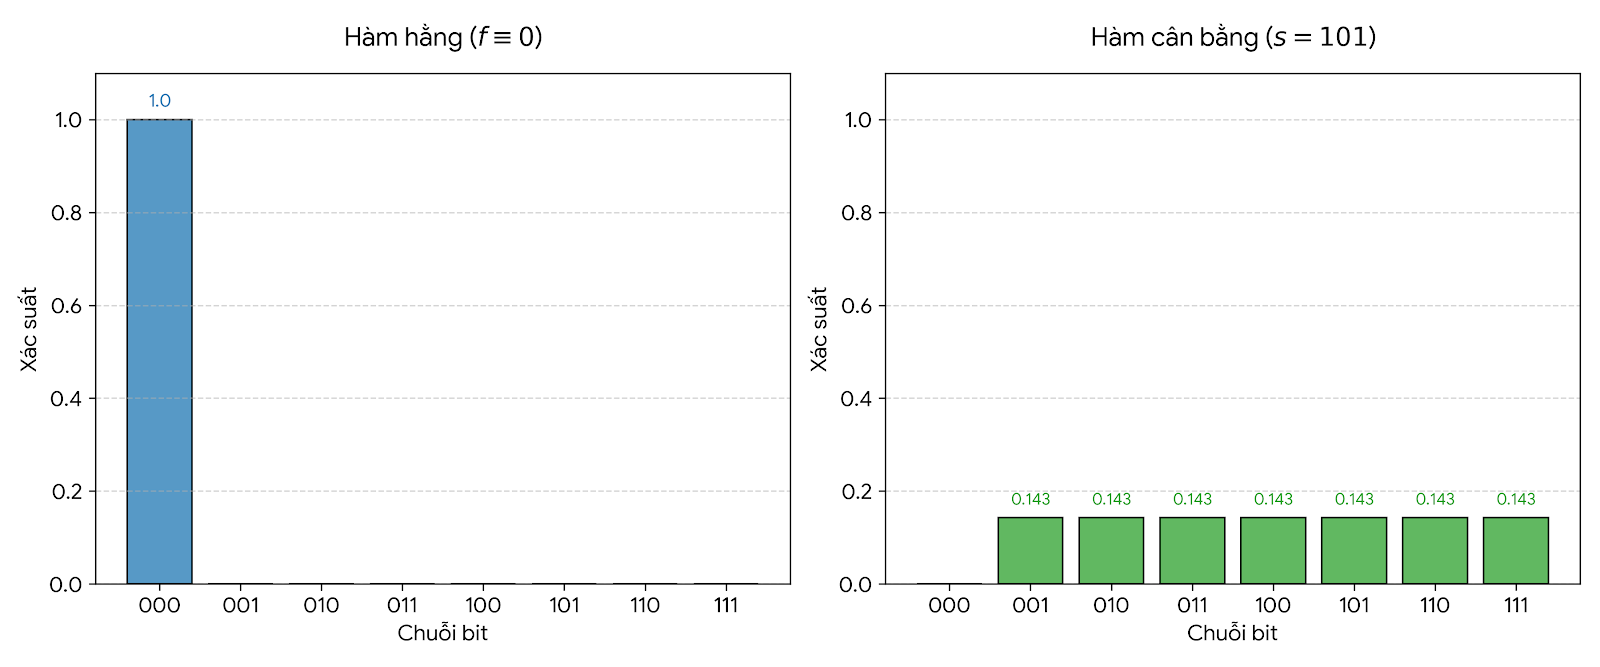
\includegraphics[width=1\textwidth]{assets/histogram.png}
    \caption{Biểu đồ xác suất đo của thuật toán Deutsch--Jozsa với $n=3$.}
    \label{fig:histogram-n3}
\end{figure}

Kết quả đầy đủ cho $n = 1, \ldots, 5$ được tổng hợp trong bảng sau.

\begin{table}[H]
\centering

\caption{Xác suất đo $P(|0\rangle^{\otimes n})$ của thuật toán Deutsch--Jozsa
         theo số qubit $n$}
\renewcommand{\arraystretch}{1.4}
\begin{tabular}{ccccc}
\hline
\multirow{2}{*}{$n$}
  & \multirow{2}{*}{Không gian ($2^n$)}
  & \multicolumn{2}{c}{$P(|0\rangle^{\otimes n})$}
  & \multirow{2}{*}{Kết luận} \\
\cline{3-4}
& & Hàm hằng & Hàm cân bằng & \\
\hline
$1$ & $2$  & $1.000$ & $0.000$ & Đúng \\
$2$ & $4$  & $1.000$ & $0.000$ & Đúng \\
$3$ & $8$  & $1.000$ & $0.000$ & Đúng \\
$4$ & $16$ & $1.000$ & $0.000$ & Đúng \\
$5$ & $32$ & $1.000$ & $0.000$ & Đúng \\
\hline
\end{tabular}

\end{table}

Kết quả trên cho thấy $P(|0\rangle^{\otimes n}) = 1$
với mọi hàm hằng và $P(|0\rangle^{\otimes n}) = 0$ với mọi hàm cân bằng,
bất kể $n$.

%────────────────────────────────────────────────────────────────────────────
\subsection*{So sánh với lý thuyết đã chứng minh}
%────────────────────────────────────────────────────────────────────────────

Kết quả mô phỏng xác nhận đầy đủ ba kết luận lý thuyết:

\textbf{(i) Tính đúng đắn tuyệt đối.} Với mọi $n$ từ $1$ đến $5$ và mọi
oracle thử nghiệm, thuật toán cho kết quả đúng với xác suất $1$ -- không
có trường hợp sai.

\textbf{(ii) Giao thoa tăng cường và triệt tiêu.} Toàn bộ xác suất tập trung tại
$|0\rangle^{\otimes n}$ (hàm hằng) hoặc hoàn toàn triệt tiêu tại đó (hàm
cân bằng).

\textbf{(iii) Tính độc lập với $n$.} Bảng 3.2 cho thấy kết
quả không phụ thuộc vào $n$: dù không gian trạng thái tăng từ $2^1 = 2$
lên $2^5 = 32$, thuật toán vẫn chỉ cần đúng một lần truy vấn oracle --
minh họa trực tiếp ưu thế $O(1)$ so với $O(2^{n-1})$ của thuật toán cổ
điển.

\subsection*{Kết luận cuối Chương 3}
Chương này đã hoàn thành mục tiêu trung tâm của khóa luận: phân tích
toán học đầy đủ và kiểm chứng thực nghiệm thuật toán Deutsch--Jozsa.
Bài toán được phát biểu chính xác, cơ chế phase kickback được chứng minh,
và kết quả trung tâm -- xác suất đo $P(|0\rangle^{\otimes n})$ bằng $1$
với hàm hằng và bằng $0$ với hàm cân bằng -- được thiết lập bằng chứng
minh toán học chặt chẽ. Ưu thế $O(1)$ so với $O(2^{n-1})$ của thuật toán
cổ điển được lý giải thông qua cơ chế giao thoa tăng cường và triệt tiêu,
và được xác nhận độc lập qua mô phỏng số với Qiskit cho $n = 1, \ldots, 5$.

\chapter*{}
\begin{center}
    {\fontsize{20}{24}\selectfont\bfseries KẾT LUẬN}
\end{center}
\addcontentsline{toc}{chapter}{Kết luận}
\vspace{1cm}
Khóa luận này đã xây dựng một nội dung hoàn chỉnh từ nền tảng toán học
đến phân tích lý thuyết và kiểm chứng thực nghiệm của thuật toán
Deutsch--Jozsa. Cụ thể, Chương~1 thiết lập cơ sở toán học cần thiết gồm
không gian Hilbert, các toán tử Hermitian và unitary, Định lý phổ, tích
tensor và bốn tiên đề Dirac--von Neumann, trong đó cơ chế giao thoa lượng
tử được phân tích từ nền tảng tiên đề và theo dõi xuyên suốt đến bước cuối
của thuật toán. Chương~2 triển khai cơ sở toán học thành mô hình tính toán
lượng tử cụ thể qua qubit, các cổng lượng tử cơ bản và cấu trúc mạch.
Chương~3 phát biểu bài toán Deutsch--Jozsa, chứng minh chặt chẽ kết quả
trung tâm rằng thuật toán phân biệt hàm hằng và hàm cân bằng với xác suất
$1$ trong đúng một lần truy vấn oracle, và kiểm chứng kết quả đó qua mô
phỏng số với Qiskit cho $n = 1, \ldots, 5$.

Bên cạnh những kết quả đạt được, khóa luận còn một số hạn chế cần thừa
nhận. Về phạm vi thuật toán, Deutsch--Jozsa giải quyết một bài toán có điều
kiện và ưu thế tuyệt đối $O(1)$ so với $O(2^{n-1})$ chỉ đúng với thuật
toán cổ điển tất định; nếu cho phép xác suất, ưu thế này thu hẹp đáng kể.

Trong tương lai, đề tài có thể được phát triển theo hướng mở rộng sang các
thuật toán lượng tử có ứng dụng thực tiễn hơn. Cụ thể, thuật toán Grover
khai thác cùng cơ chế giao thoa để tìm kiếm với độ phức tạp $O(\sqrt{N})$,
biến đổi Fourier lượng tử (QFT) tổng quát hóa Hadamard transform đã xây
dựng trong khóa luận, và thuật toán Shor sử dụng QFT để phân tích nhân tử
với hiệu quả vượt trội so với mọi thuật toán cổ điển đã biết.

\chapter*{}
\addcontentsline{toc}{chapter}{Tài liệu tham khảo}
\begin{thebibliography}{9}

    \bibitem{ref1} D. Deutsch (1985). ``Quantum theory, the Church-Turing principle and the universal quantum computer." \textit{Proceedings of the Royal Society of London A,} 400, 97–117.

    \bibitem{ref2} D. Deutsch \& R. Jozsa (1992). ``Rapid solution of problems by quantum computation." \textit{Proceedings of the Royal Society of London A}, 439, 553–558. 
    
    \bibitem{ref3} G. Kuperberg (2005). \textit{``A concise introduction to quantum probability, quantum mechanics, and quantum computation."} 

    \bibitem{ref4} H. Maassen. \textit{``Quantum Probability, Quantum Information Theory, Quantum Computing."}

    \bibitem{ref5} M. A. Nielsen \& I. L. Chuang (2010). \textit{``Quantum Computation and Quantum Information."} Cambridge University Press.

\end{thebibliography}

\chapter*{}
\begin{center}
    {\fontsize{20}{24}\selectfont\bfseries PHỤ LỤC}
\end{center}
\addcontentsline{toc}{chapter}{Phụ lục}
\fancyhead[L,R]{} % Xóa header cho phần phụ lục
\section*{Phụ lục 1: Mã nguồn Python/Qiskit}
\addcontentsline{toc}{section}{Phụ lục 1: Mã nguồn Python/Qiskit}

Toàn bộ mã nguồn Python/Qiskit cho mô phỏng thuật toán Deutsch--Jozsa
được trình bày tại: \url{https://github.com/tdattm/Deutsch-Jozsa.git}

\section*{Phụ lục 2: Các cổng lượng tử và ký hiệu mạch}
\addcontentsline{toc}{section}{Phụ lục 2: Các cổng lượng tử và ký hiệu mạch}
\begin{figure}[H]
    \centering
    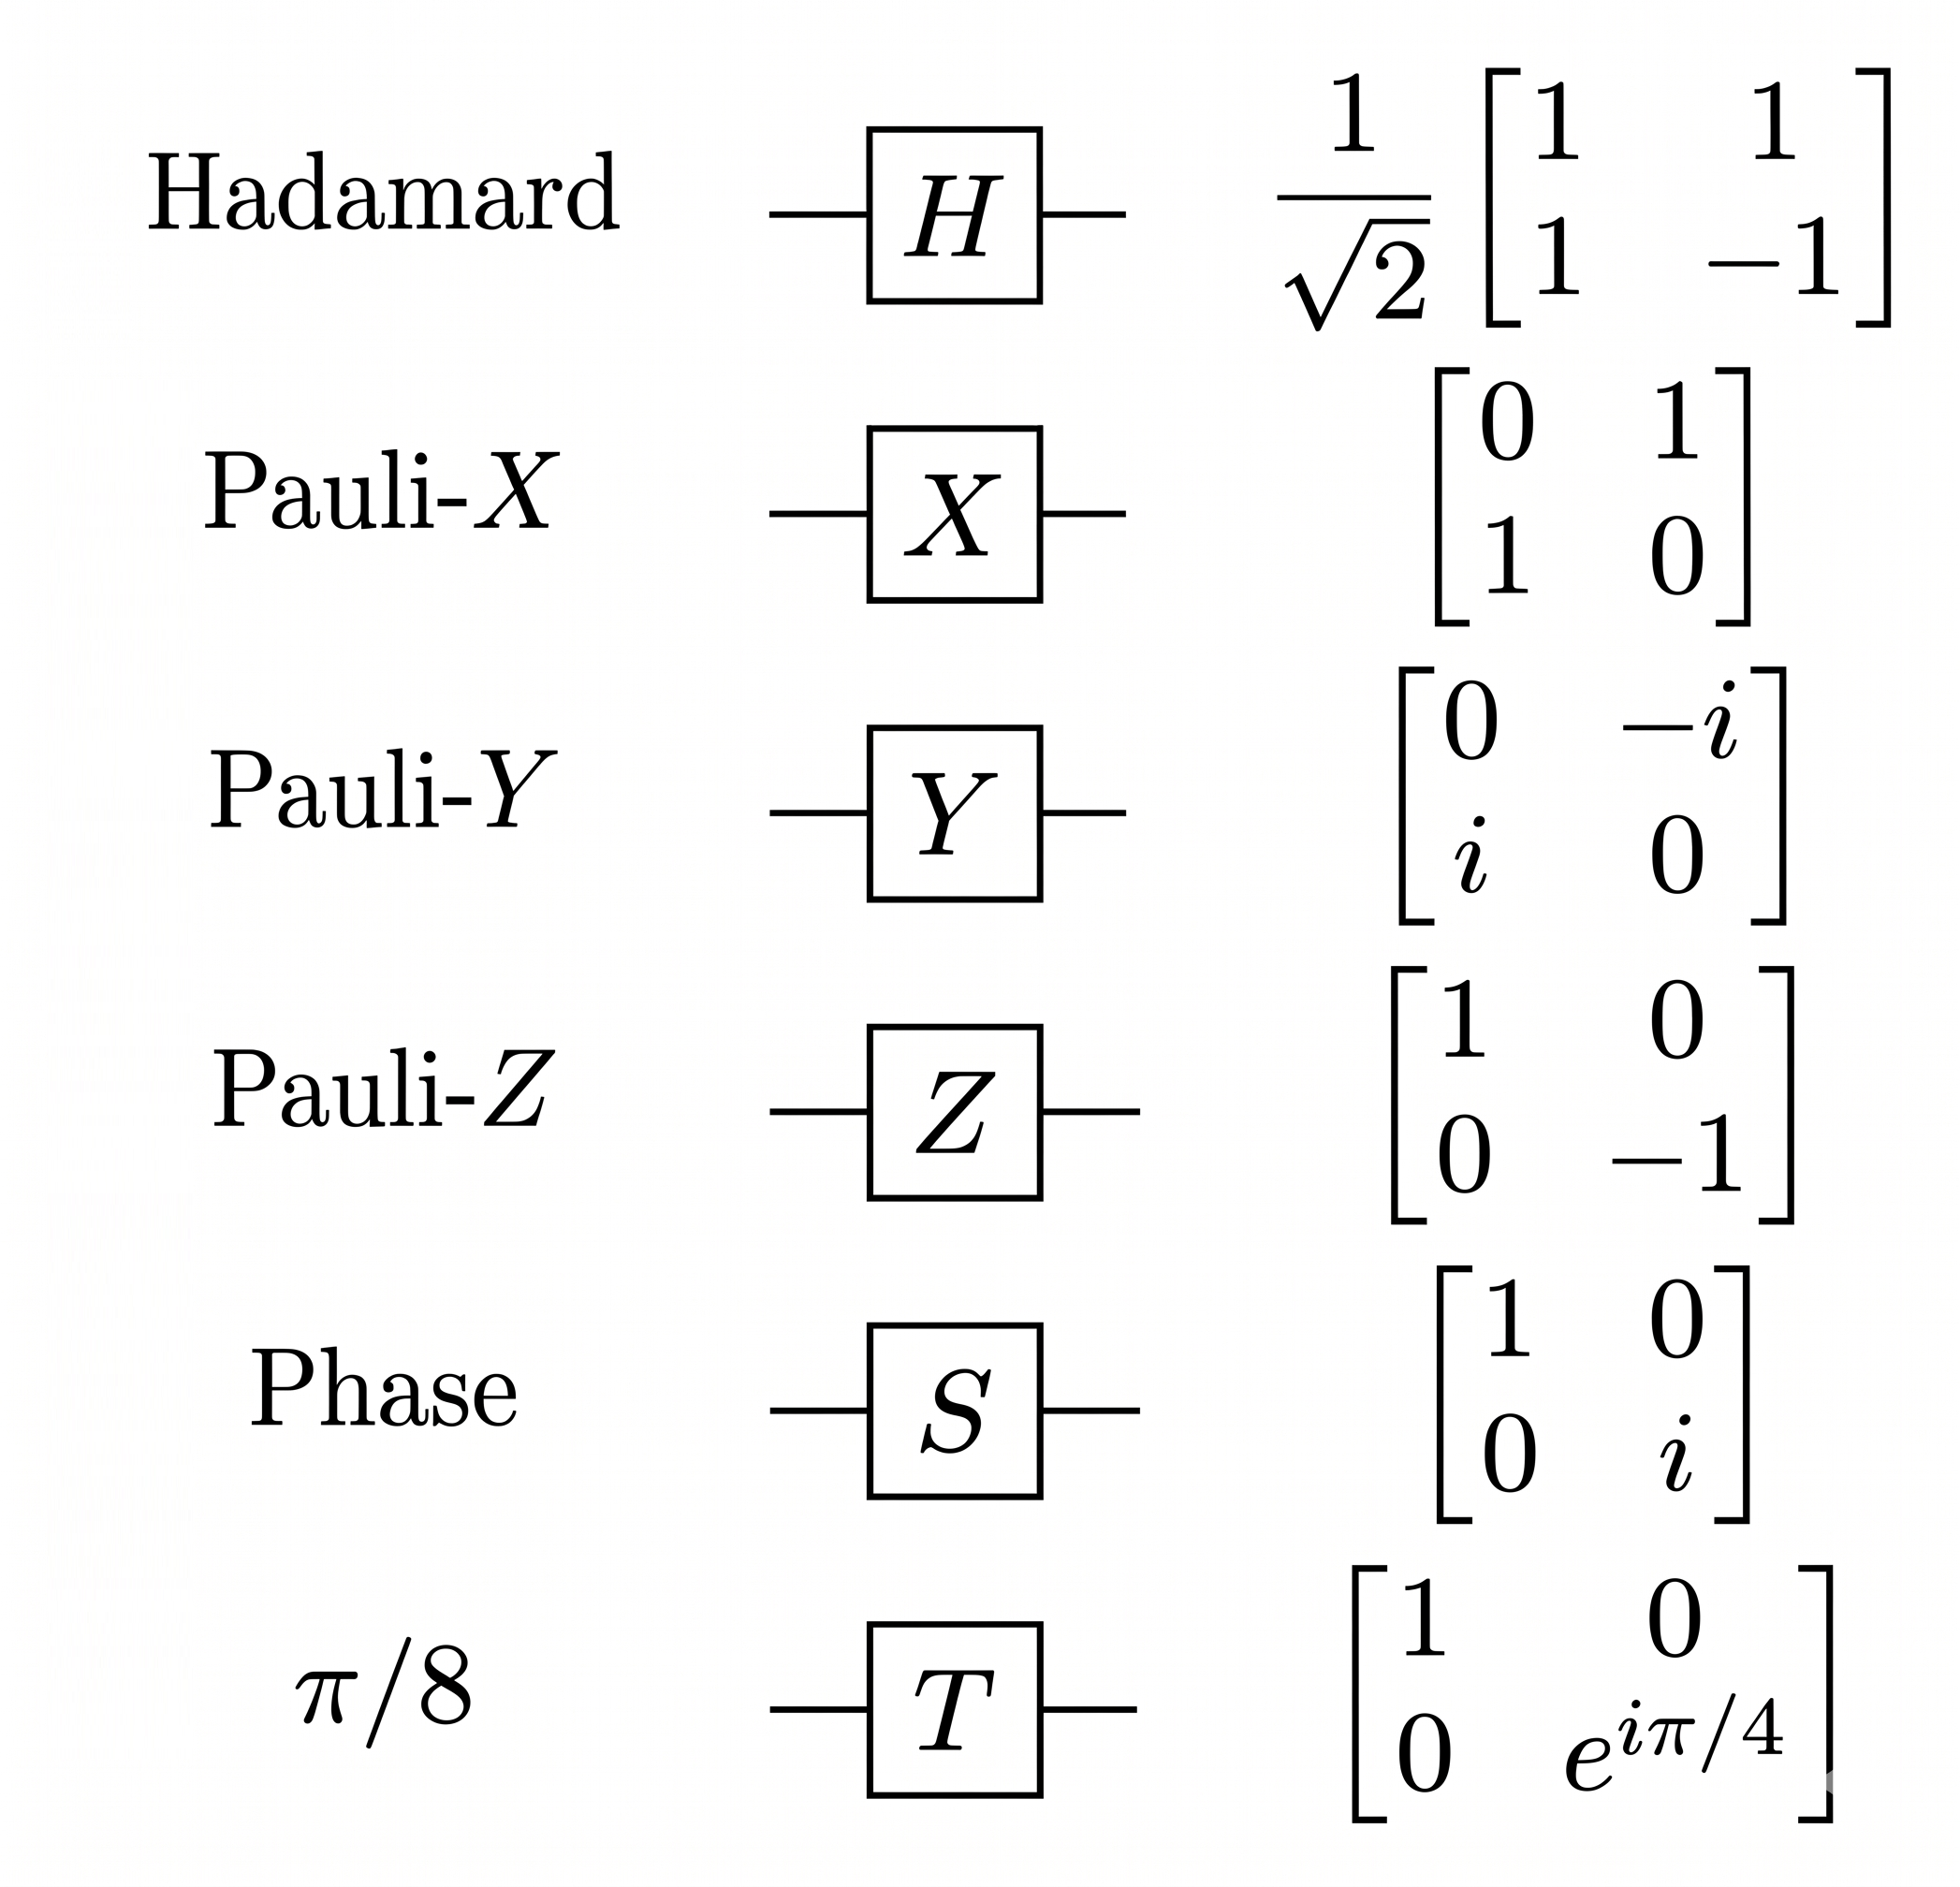
\includegraphics[width=0.7\textwidth]{assets/quantumGates-1.png} 
\end{figure}

\begin{figure}[H]
    \centering
    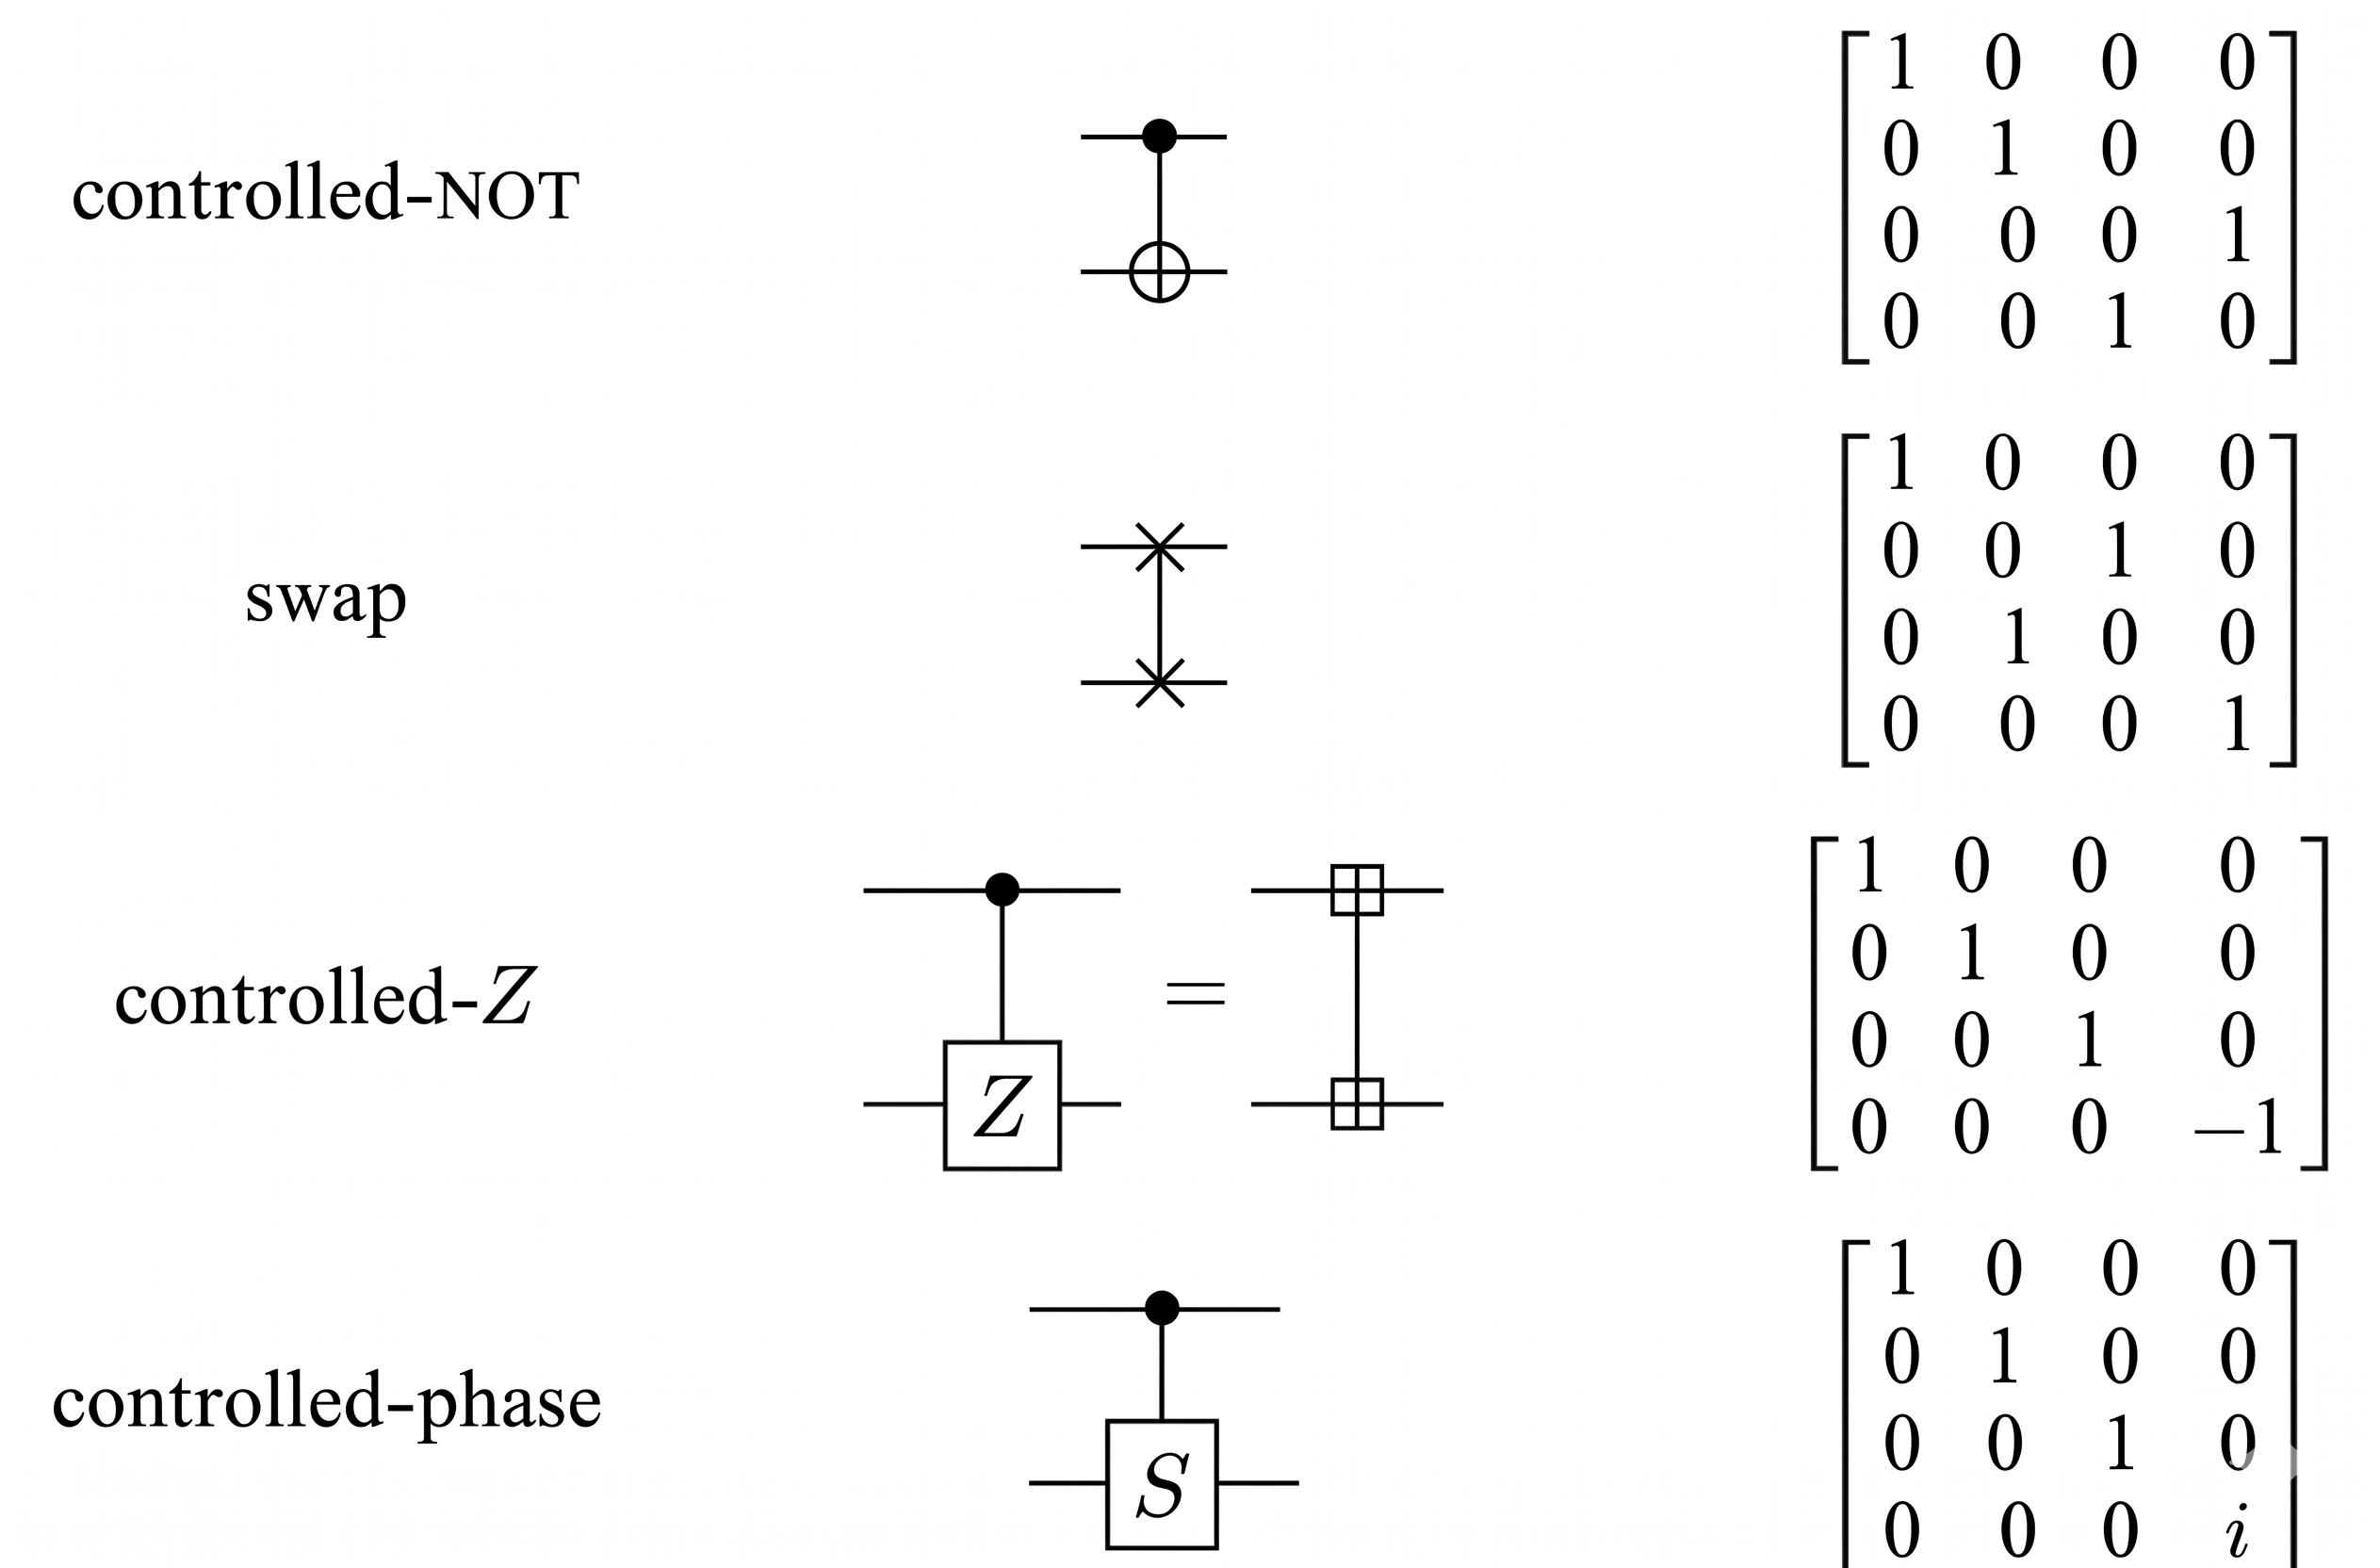
\includegraphics[width=0.9\textwidth]{assets/quantumGates-2.png} 
\end{figure}

\begin{figure}[H]
    \centering
    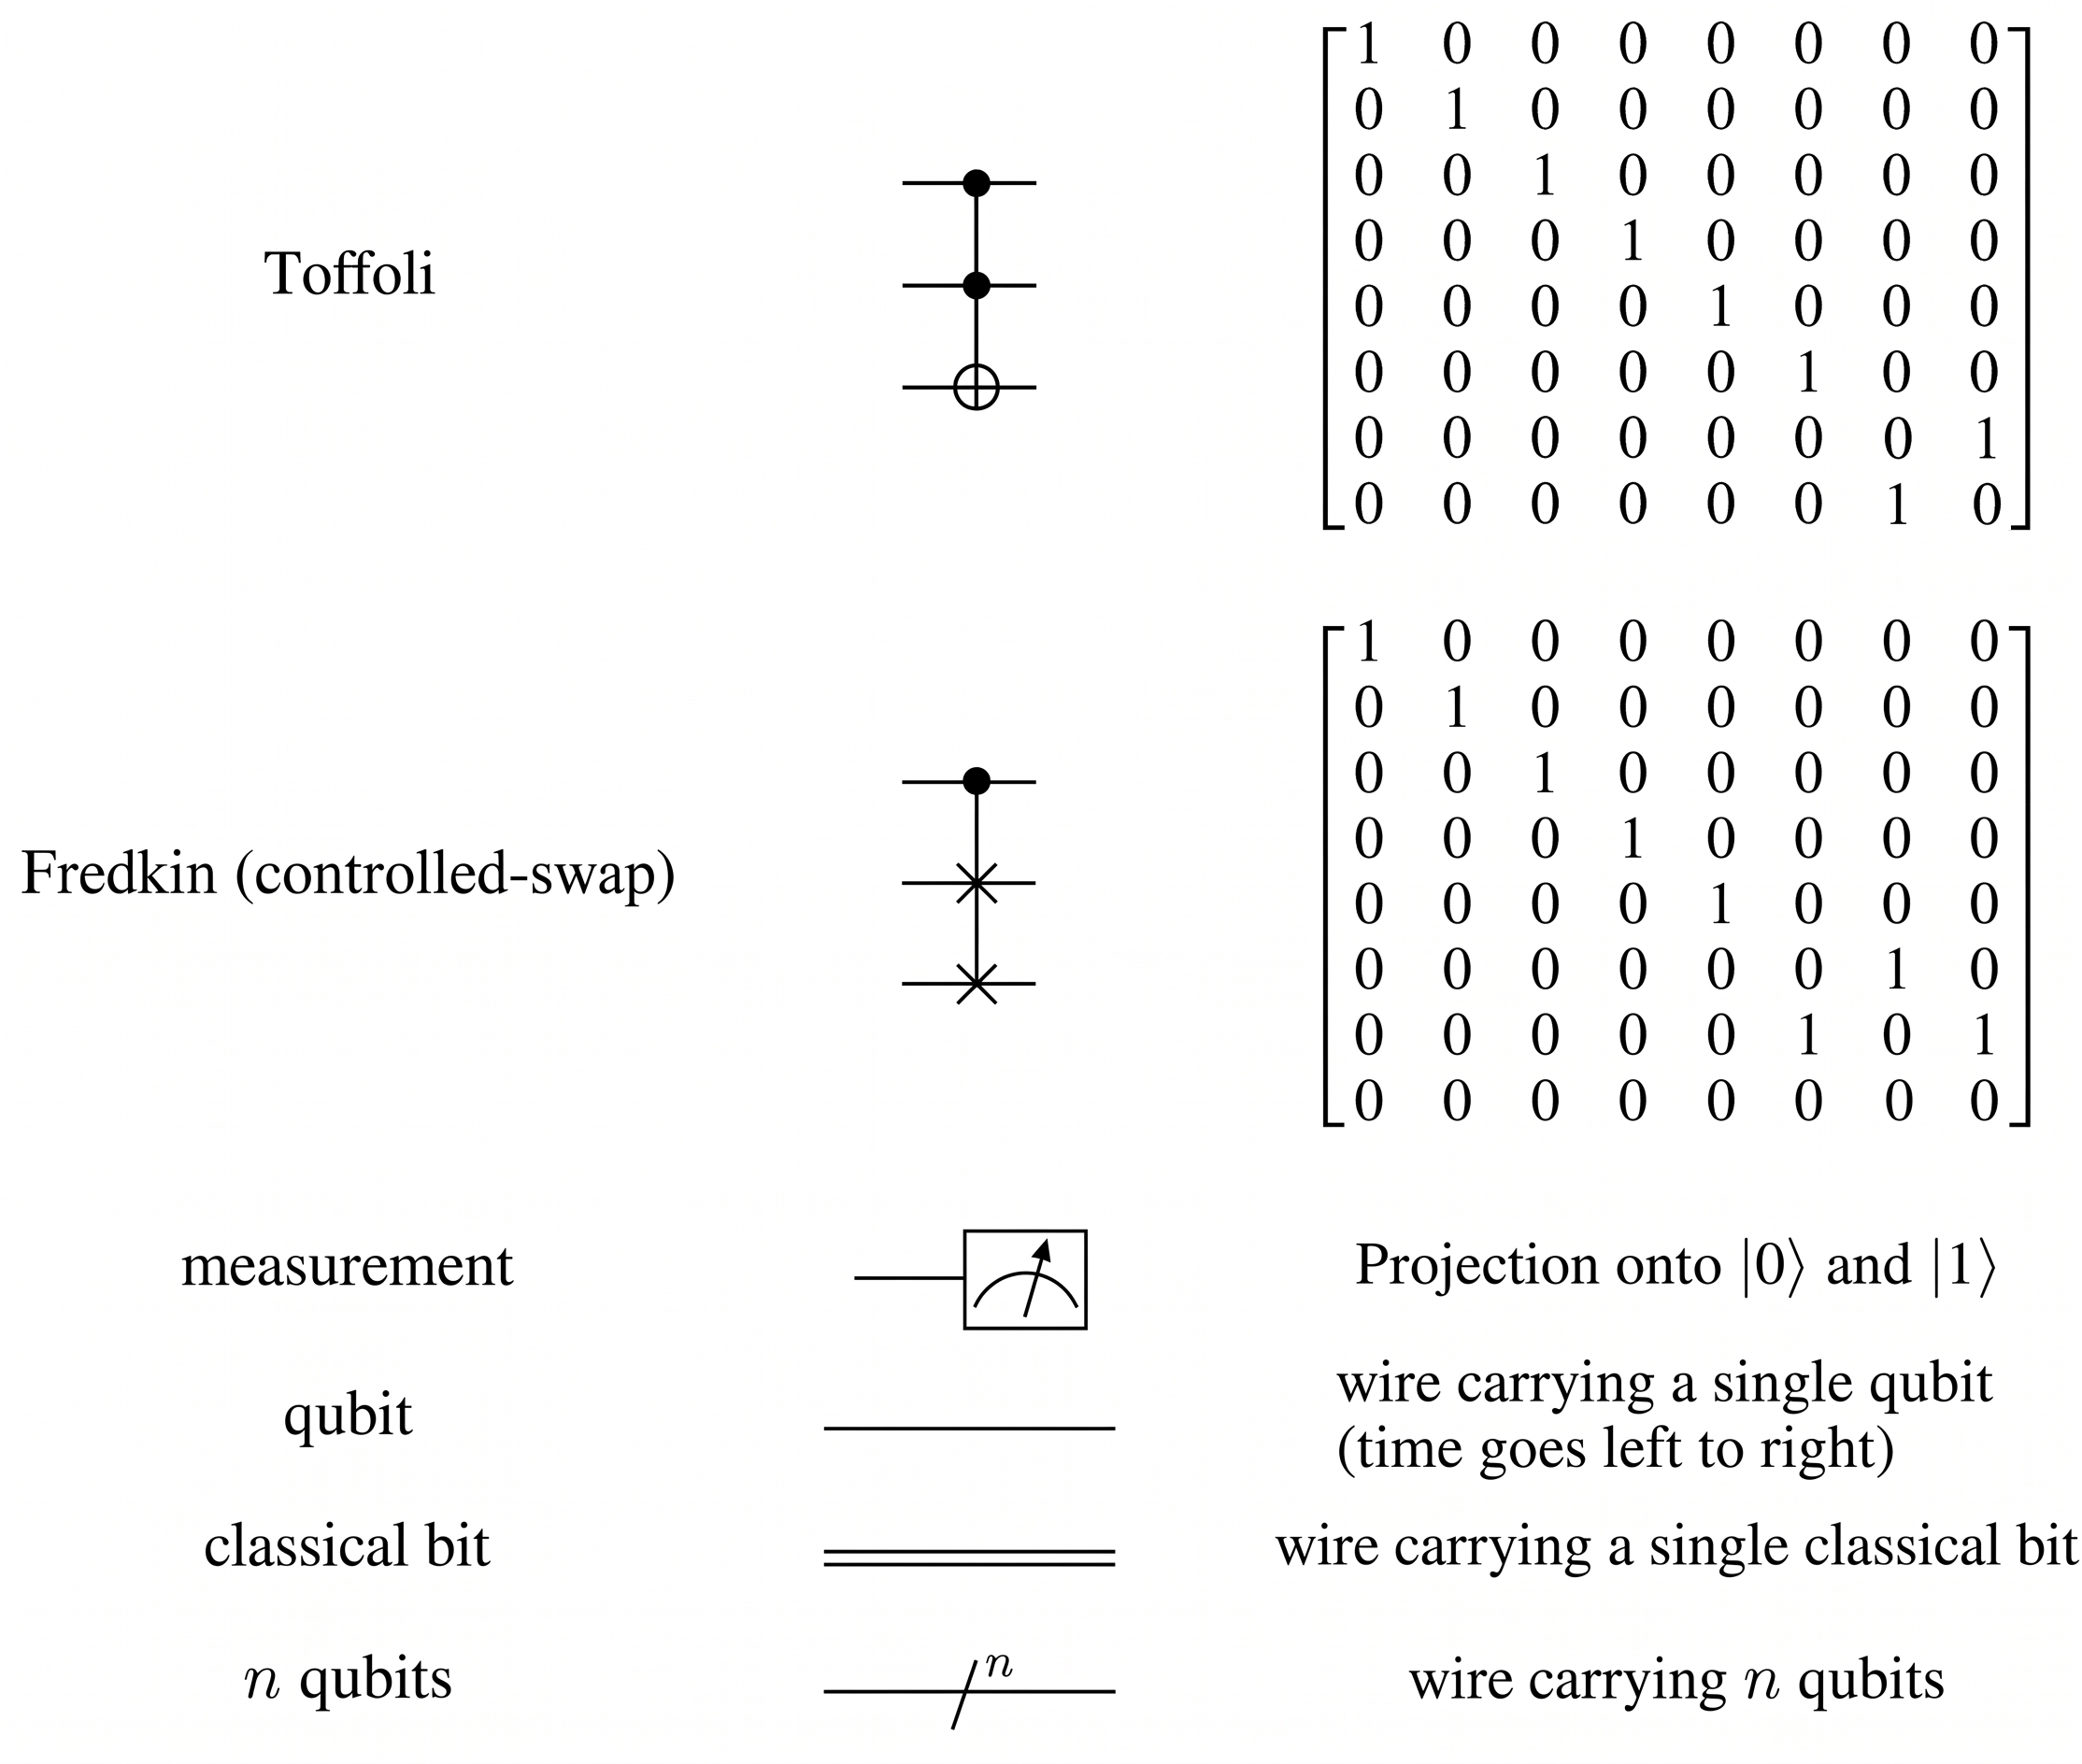
\includegraphics[width=0.9\textwidth]{assets/quantumGates-3.png} 
    \caption{Ký hiệu mạch các cổng lượng tử phổ biến.}
    \vspace{0.2cm}
    \small\textit{Nguồn: \cite{ref5}}
\end{figure}

\section*{Phụ lục 3: Biểu diễn số phức và công thức Euler}
\addcontentsline{toc}{section}{Phụ lục 3: Biểu diễn số phức và công thức Euler}
\label{app:complex}

Phụ lục này tóm tắt cách chuyển đổi một số phức từ dạng đại số sang dạng Euler,
phục vụ cho việc hiểu khái niệm pha toàn cục và pha tương đối trong
mục~\ref{sec:qubit}.

Cho số phức $\alpha = a + bi$ với $a, b \in \mathbb{R}$, trong đó $a$ là phần
thực và $b$ là phần ảo. Số phức này có thể được biểu diễn trực quan như một điểm
(hoặc vectơ) trên mặt phẳng phức, với trục hoành là trục thực và trục tung là
trục ảo.

\begin{figure}[htbp]
    \centering
    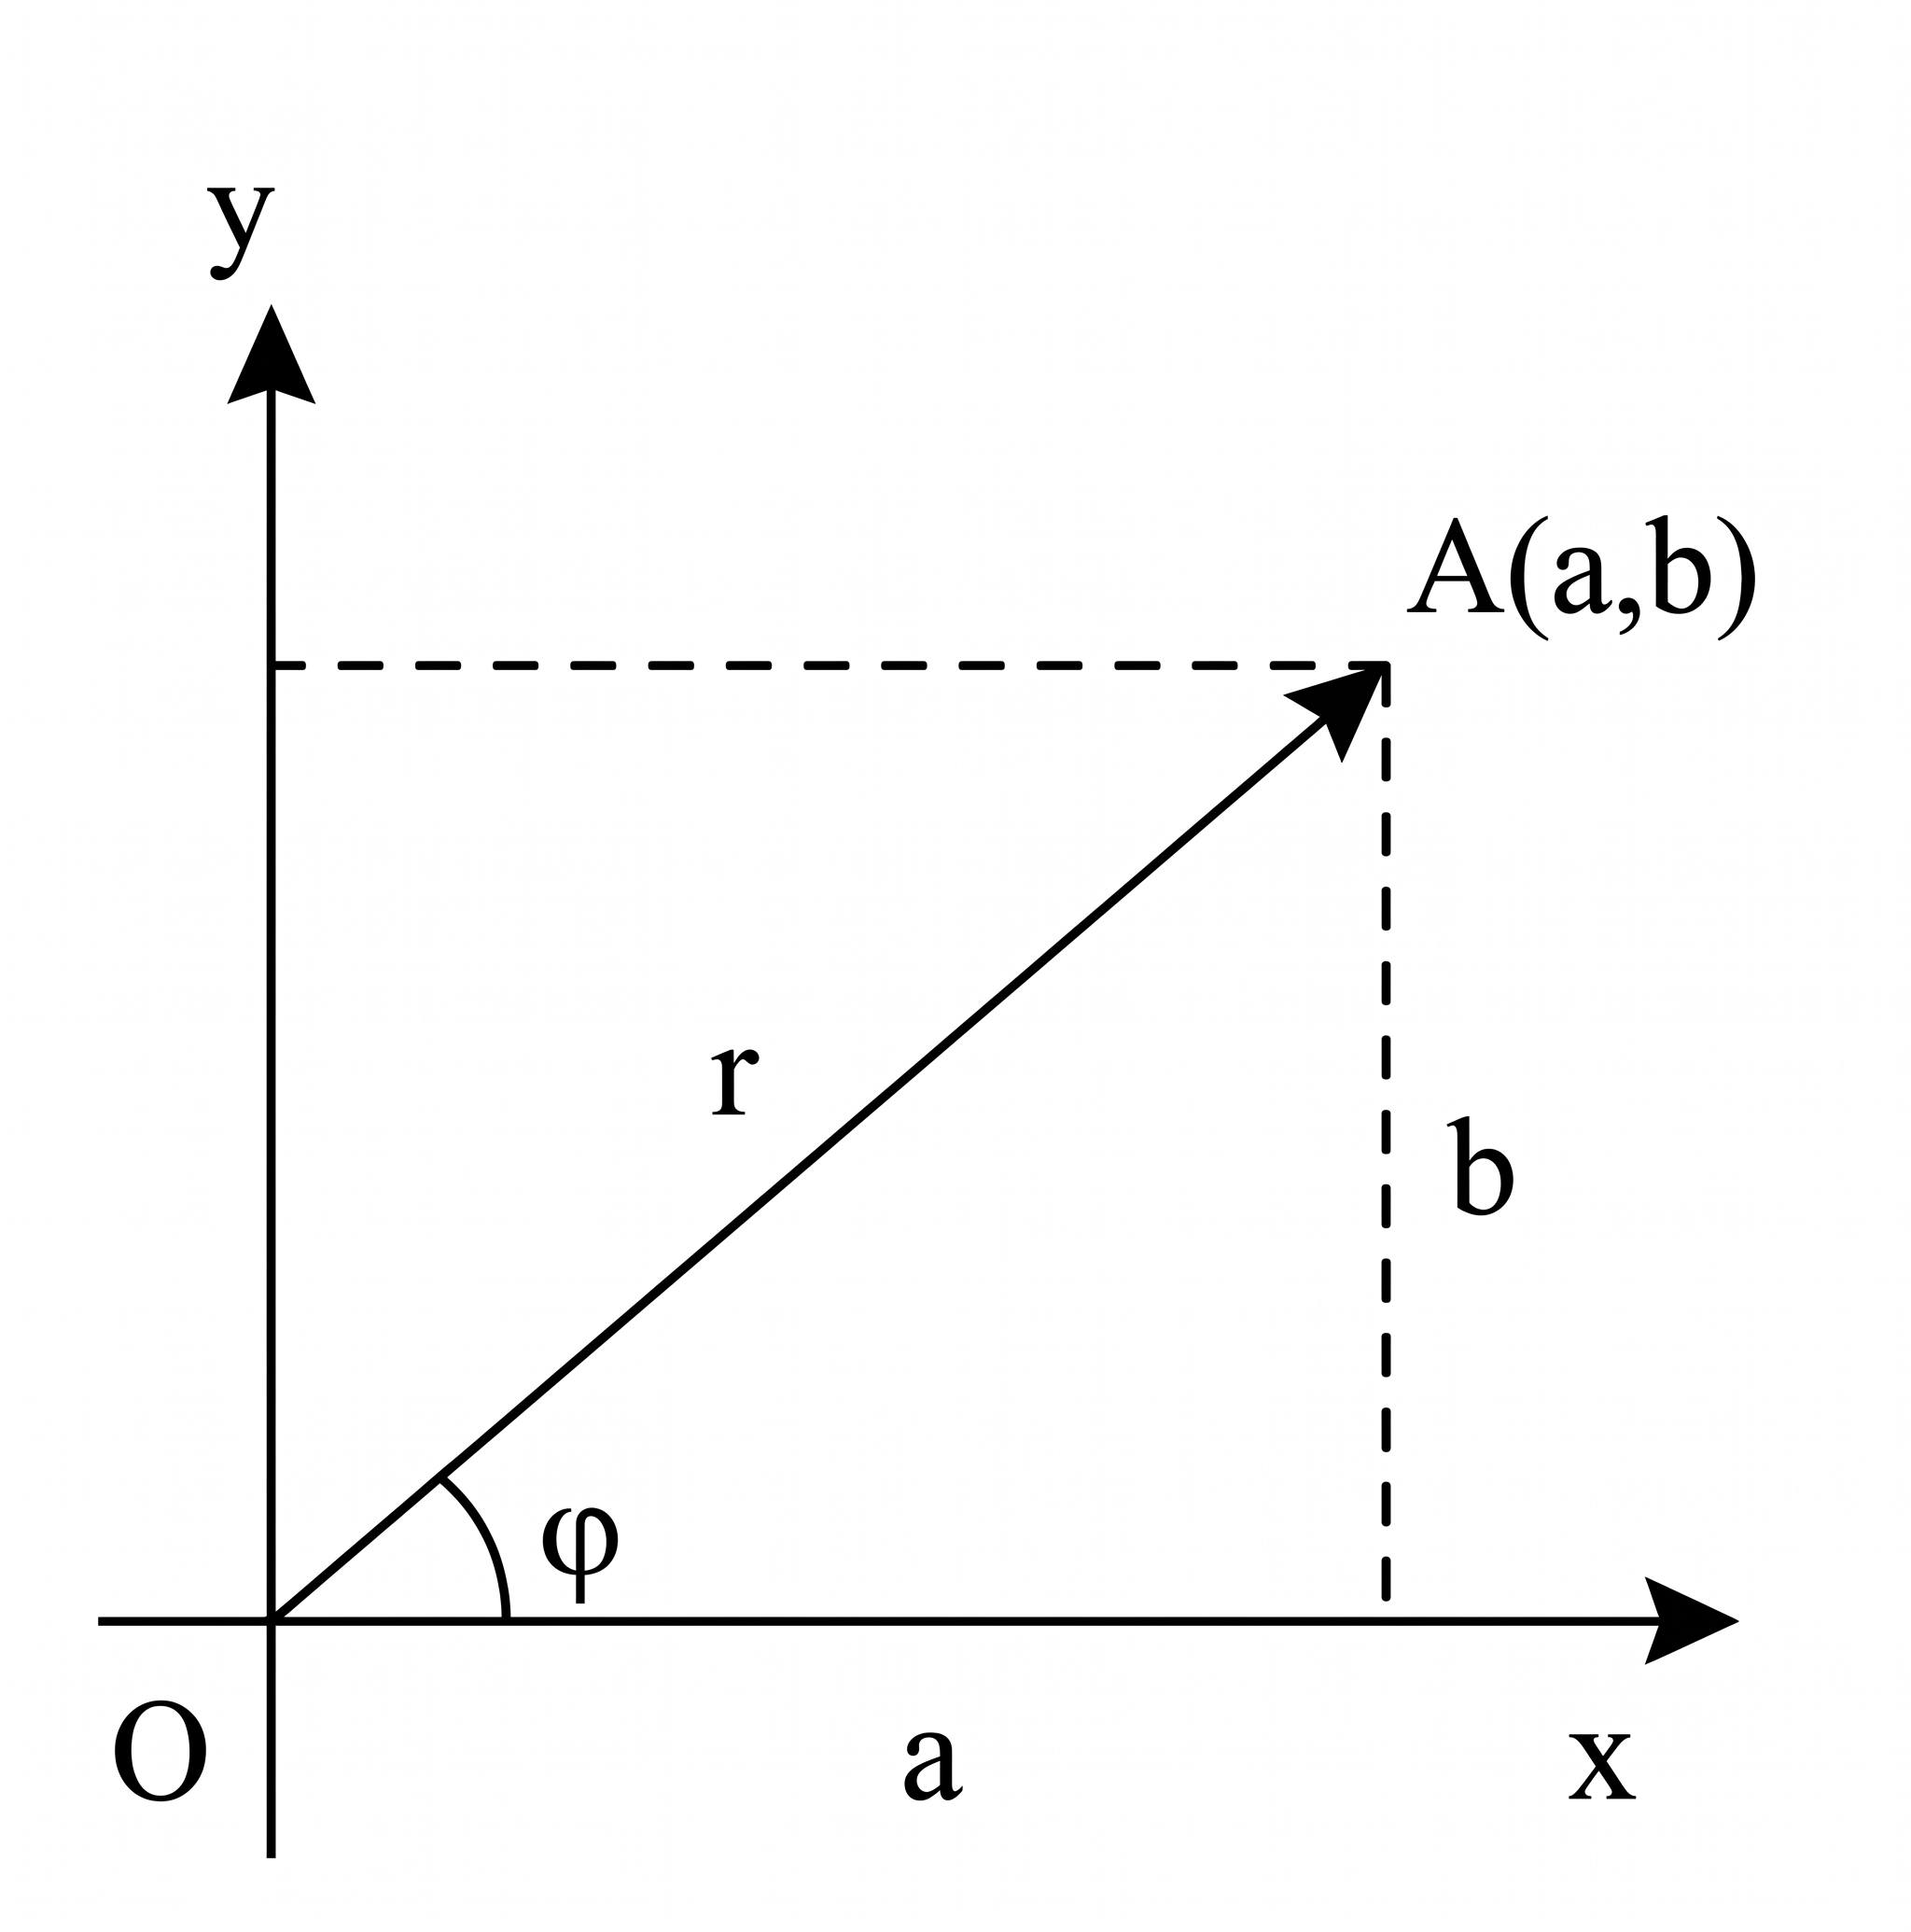
\includegraphics[width=0.5\textwidth]{assets/sophuc.png}
    \caption{Biểu diễn số phức $\alpha = a + bi$ trên mặt phẳng phức.}
    \label{fig:sophuc}
    \vspace{0.2cm}
    \small\textit{Nguồn: Khoa Vật lý, Đại học Sư phạm Tp.HCM.}
\end{figure}

\paragraph{(a) Dạng lượng giác.}
Từ hình học mặt phẳng, vectơ $(a, b)$ có độ dài $r$ và tạo với trục thực một góc
$\theta$, nên các thành phần được biểu diễn qua:
$$a = r\cos\theta, \qquad b = r\sin\theta,$$
trong đó:
$$r = |\alpha| = \sqrt{a^2 + b^2} \quad \text{(môđun)},
\qquad \tan\theta = \frac{b}{a} \quad \text{($\theta$: argument)}.$$
Thay vào $\alpha = a + bi$, ta được \textbf{dạng lượng giác}:
$$\alpha = r(\cos\theta + i\sin\theta).$$

\paragraph{(b) Dạng Euler.}
Công thức Euler khẳng định rằng với mọi $\theta \in \mathbb{R}$:
$$e^{i\theta} = \cos\theta + i\sin\theta.$$
Thay vào dạng lượng giác, số phức $\alpha$ được viết gọn thành
\textbf{dạng Euler}:
\begin{equation}
    \alpha = r\,e^{i\theta}.
    \label{eq:euler}
\end{equation}

% ===============================================================
\section*{Phụ lục 4: Nguồn gốc phương trình tham số hóa mặt cầu Bloch}
\addcontentsline{toc}{section}{Phụ lục 4: Nguồn gốc phương trình tham số hóa mặt cầu Bloch}

Phụ lục này trình bày chi tiết cách dẫn xuất phương trình tham số hóa trạng thái
qubit trên mặt cầu Bloch của phương trình~\eqref{eq:bloch-param} từ dạng tổng quát phương trình~\eqref{eq:qubit}. Nội dung này thuộc vào mục 2.1 của chương 2.

% ---------------------------------------------------------------
\paragraph{(a) Đếm bậc tự do thực}

Trạng thái tổng quát của một qubit là
\[
    |\psi\rangle = \alpha|0\rangle + \beta|1\rangle,
    \quad \alpha, \beta \in \mathbb{C},
\]
trong đó $\alpha$ và $\beta$ mỗi số phức mang hai bậc tự do thực (phần thực và
phần ảo), nên tổng cộng có \emph{bốn} bậc tự do thực. Hai ràng buộc lần lượt
loại bỏ hai trong số đó:

\begin{enumerate}
    \item \textbf{Điều kiện chuẩn hóa} $|\alpha|^2 + |\beta|^2 = 1$ là một
          phương trình thực, loại bỏ một bậc tự do.
    \item \textbf{Pha toàn cục} không có ý nghĩa vật lý: hai trạng thái
          $|\psi\rangle$ và $e^{i\gamma}|\psi\rangle$ cho cùng xác suất đo
          trong mọi cơ sở, nên được đồng nhất về mặt vật lý. Điều này loại
          bỏ thêm một bậc tự do.
\end{enumerate}

Sau hai ràng buộc, còn lại đúng \textbf{hai bậc tự do thực} -- vừa đủ để biểu
diễn bằng hai góc $(\theta, \phi)$ trên mặt cầu đơn vị trong $\mathbb{R}^3$.


% ---------------------------------------------------------------
\paragraph{(b) Tham số hóa modulus bằng góc lượng giác}

Viết $\alpha$ và $\beta$ theo dạng cực:
\[
    \alpha = r_\alpha \, e^{i\varphi_\alpha}, \qquad
    \beta  = r_\beta  \, e^{i\varphi_\beta},
    \quad r_\alpha, r_\beta \geq 0.
\]
Điều kiện chuẩn hóa trở thành $r_\alpha^2 + r_\beta^2 = 1$, có dạng hệ thức
Pythagore. Đặt:
\[
    r_\alpha = \cos\frac{\theta}{2}, \qquad
    r_\beta  = \sin\frac{\theta}{2}, \qquad \theta \in [0, \pi].
\]
Lý do chọn $\frac{\theta}{2}$ thay vì $\theta$: khi $\theta$ chạy từ $0$ đến $\pi$,
góc $\frac{\theta}{2}$ chạy từ $0$ đến $\pi/2$, đảm bảo $\cos(\frac{\theta}{2}) \geq 0$ và
$\sin(\frac{\theta}{2}) \geq 0$, tức $r_\alpha, r_\beta \geq 0$ luôn thỏa mãn mà
không cần ràng buộc thêm. Thay vào trạng thái:
\[
    |\psi\rangle
    = \cos\frac{\theta}{2}\,e^{i\varphi_\alpha}|0\rangle
    + \sin\frac{\theta}{2}\,e^{i\varphi_\beta}|1\rangle.
\]

% ---------------------------------------------------------------
\paragraph{(c) Loại bỏ pha toàn cục}

Nhân toàn bộ $|\psi\rangle$ với $e^{-i\varphi_\alpha}$ -- đây là phép nhân
pha toàn cục, không thay đổi bất kỳ xác suất đo nào:
\[
    |\psi\rangle \;\sim\; e^{-i\varphi_\alpha}|\psi\rangle
    = \cos\frac{\theta}{2}|0\rangle
    + \sin\frac{\theta}{2}\,e^{i(\varphi_\beta - \varphi_\alpha)}|1\rangle.
\]
Đặt $\phi = \varphi_\beta - \varphi_\alpha \in [0, 2\pi)$ là \textbf{pha tương
đối} -- bậc tự do pha duy nhất còn ý nghĩa vật lý. Ta thu được:
\[
    |\psi\rangle = \cos\frac{\theta}{2}|0\rangle
                + e^{i\phi}\sin\frac{\theta}{2}|1\rangle,
\]
đúng với phương trình~\eqref{eq:bloch-param}.

\end{document}